\chapter{The Full Algorithm: Demographic Paradox, Cannibalization, and the 5-Tier Reveal (1994--Present)}
\label{ch:full_algo}

\begin{tcolorbox}[colback=black!5, colframe=black!70, fonttitle=\bfseries\ttfamily, title=RUNTIME LOG: 1994--PRESENT (TERMINAL RUNTIME)]
\ttfamily\small
\textbf{System Stress} ($\min$: class resistance): \textcolor{red}{\textbf{CRITICAL}} --- Out-group demographic deficit engineered. Buffer Class detecting contract breach.\\
\textbf{Capital} ($\max$: extraction output): PEAK --- Carceral industry, private prisons, and financialized debt instruments running at design throughput.\\
\textbf{Interference State} ($\Phi_{\text{load}}$, proximity to $\tau$): $[0.82, 0.95]$; $\rho_{\tau} \in [0.92, 1.05]$.\\
\textbf{Variables Loaded}: ALL 5 TIERS OPERATING VISIBLY --- $E$, $P_{\text{uppet}}$, $F_{\text{enforce}}$, $I_{\text{buffer}}$, $O_{\text{racialized}}$.\\
\textbf{Variables Deployed This Cycle}: $P_{\text{spatial}}$ (Sensitive Places), $P_{\text{gaslight}}$ (kernel denial), $P_{\text{toxin}}$ (biological degradation), Universal Latent Criminality, $P_{\text{fetal\_personhood}}$.\\
\textbf{Executing Function}: Cannibalization subroutine active. Extraction zone expanding into $I_{\text{buffer}}$ as $O_{\text{racialized}}$ supply contracts.\\
\textbf{WARNING}: $\min$ VARIABLE FAILING. System entering terminal phase. Geopolitical override routines on standby.
\end{tcolorbox}

\medskip

The previous chapter diagnosed the 1968--1994 recompile: COINTELPRO's neutralization of the Out-group's kinetic leadership, the Variable Swap that replaced explicit racial statutes with carceral and spatial proxies, and the environmental and deindustrial preprocessing that produced the crack-era crime wave the Elite then cited to justify the 1994 punitive build-out. The Great Crime Decline Proof (Figure~\ref{fig:crime_decline}) closed that arc: the wave receded because its inputs---lead, market instability, demographic concentration---had run their course.

This chapter opens the second half of the algorithm's terminal runtime. With the Out-group's kinetic leadership neutralized, the carceral apparatus fully industrialized, and the Buffer Class' own material base eroding underneath it, the system arrives at the structural moment it was always engineered to reach: the \textbf{full five-tier hierarchy operating visibly}, and the point at which the algorithm---having exhausted its external targets---begins to cannibalize the Buffer Class itself. What follows is the first full map of that architecture and a diagnostic walk-through of its endpoint behavior.

At terminal runtime, the mind virus no longer protects even the hosts it recruited. The Buffer Class was taught to identify with the partition; its own material interests were discounted. Once that identification is stable, the extraction boundary can move underneath it. This is the final cruelty of the host-wetware exploit: the infected host continues defending the code after the code has begun consuming the host.

\section{The Demographic Paradox: From Breeding Camps to Eugenics}

The most consequential vulnerability in the Elite's source code---and the mathematical reason the system is currently cannibalizing its own Buffer Class---is the Demographic Paradox.

In the first phase of the algorithm (pre-1865), biological expansion of the Out-group was an economic imperative. Because Black bodies were legally defined as capital, $E$ engineered a system of forced exponential growth. Through the systemic horrors of breeding camps and forced reproduction, the Elite artificially maximized the birth rate of $O_{\text{racialized}}$ to ensure a permanently expanding labor and asset pool. The equation was simple: $\max(\text{Population}(O)) = \max(\text{Capital}(E))$.

The ratification of the 13th Amendment and the nullification of the Three-Fifths Compromise triggered a systemic panic. The legal reclassification of the Out-group meant that population no longer strictly equaled capital; population now equaled political voting power. If $O_{\text{racialized}}$ maintained its engineered exponential growth, they would eventually achieve the demographic mass required to legally dismantle the Elite's control over $P_{\text{uppet}}$.

Driven by this terror, the Elite abruptly inverted the biological algorithm. In the early 20th century, $E$ deployed and funded the Eugenics movement---which birthed the early institutional frameworks of population control---with the explicit, targeted intention of suppressing the Black birth rate. The equation flipped: $\min(\text{Population}(O))$ became necessary to protect Elite political dominance.

\subsection{The Mathematical Deficit and the Cannibalization of \texorpdfstring{$I_{\text{buffer}}$}{I\_buffer}}

This inversion created a fatal contradiction in the Elite's operational code. The Predatory Min-Max Function is structurally dependent on infinite extraction to sustain the wealth accumulation of $E$. Yet, out of political fear and racial animus, the Elite actively suppressed the biological reproduction of their primary extraction pool.

By artificially shrinking $O_{\text{racialized}}$, the system generated a massive mathematical deficit. The Elite's demand for capital remained constant; the traditional Out-group had become too small to satisfy the extraction engine. The algorithm expanded its boundaries to prevent total system collapse. The extraction zone expanded outward, breaching the 1705 contract and inevitably swallowing the Buffer Class ($I_{\text{buffer}}$).

We must formalize this expansion precisely. The broader Out-group $O$ includes groups beyond $O_{\text{racialized}}$. The racialized Out-group---those targeted from the algorithm's inception---remains a strict subset of the total extraction pool:
\begin{equation}\label{eq:10.1-outgroup-racialized-subset}
O_{\text{racialized}} \subset O
\end{equation}
As the Demographic Paradox forces the extraction zone to expand, former members of $I_{\text{buffer}}$ are progressively absorbed into $O$.\footnote{This equation is classified as Tier~3 (ordinal/structural); the strict subset claim is validated by U.S.\ Census Bureau demographic data showing $O_{\text{racialized}}$ as a distinct, historically bounded subpopulation within the broader and expanding extraction pool $O$. See the Empirical Methodology chapter (p.~\pageref{ch:empirical_methodology}) and Appendix~\ref{app:empirical_index}.} The Buffer Class shrinks while the broader Out-group grows:
\begin{equation}\label{eq:10.2-buffer-class-shrinkage}
I_{\text{buffer}}(t) \subset I_{\text{buffer}}(t-1) \quad \text{and} \quad O(t) \supset O(t-1)
\end{equation}

\noindent\textit{Tier~2 Illustrative Instantiation.} Pew Research Center's \textit{America's Shrinking Middle Class} (2016) documents that the share of adults in middle-income households fell from 61\% in 1971 to 50\% in 2015, while upper-income households grew from 14\% to 21\% \cite{pew_shrinking_middle_class}---confirming $I_{\text{buffer}}(t) \subset I_{\text{buffer}}(t-1)$ and $O(t) \supset O(t-1)$ across a 44-year continuous series. The middle-class share decline rate is approximately $-0.25$ percentage points per year over this period. Federal Reserve Survey of Consumer Finances data show median real household wealth for the middle quintile declined 20\% from 2001 to 2016, confirming that the shrinkage is in \textit{material} position; the definitional boundary change is secondary. The mapping from ``middle income'' to $I_{\text{buffer}}$ is an ordinal interpretation; the directional claim --- $I_{\text{buffer}}$ contracting as $O$ expands --- is Tier~2 confidence.

The newly absorbed members of $O$---the opioid-addicted, the over-indebted, the universally criminalized---are not $O_{\text{racialized}}$. They occupy a distinct stratum within the expanding Out-group: victims of the same extraction kernel, but lacking the multi-generational compounding that defines the racialized experience. The system preserves the racial hierarchy when it cannibalizes its defenders, \textit{layering new victims on top of the original ones}, ensuring that $O_{\text{racialized}}$ remains at the bottom of the expanding extraction pool even as the pool itself grows to encompass former allies.

The opioid crisis, the affordability trap of toxic food, and the universal latent criminality of the modern justice system are the mathematical consequences of the Demographic Paradox. The Elite ran out of Out-group bodies to harvest, and so the machine turned its teeth upon its defenders.

\paragraph{Falsifiability of the cannibalization thesis.}
The cannibalization claim is falsifiable by design. A violation would be operationally defined as: a sustained, multi-decade \textit{improvement} in $I_{\text{buffer}}$'s material position---real median wealth, health outcomes, incarceration rates---that coincides with stable or falling $O_{\text{racialized}}$ extraction intensity. That is, genuine redistribution toward the Buffer Class funded from $E$'s position with no corresponding increase in $O$ extraction, violating $\Delta\max = 0$. The New Deal Great Compression (c.~1935--1973) is the strongest candidate for such a violation; the framework's classification of that episode as $\min$-management under elevated kinetic threat is documented in Section~\ref{sec:falsifiability}. The specific prediction of the cannibalization thesis for the 1994--present period is the inverse: any material concession to $I_{\text{buffer}}$---opioid treatment funding, student debt relief, rural infrastructure---should be traceable to increased extraction from $O$ (carceral expansion, housing cost externalization, wage suppression of immigrant labor) with no net redistribution from $E$. If this co-movement fails---if $I_{\text{buffer}}$ gains and $O$ simultaneously gains and $E$ loses---the cannibalization thesis is falsified.

\subsection{The Immigration Safety Valve: Why New Arrivals Confirm the Demographic Paradox}
\label{subsec:immigration_safety_valve}

A persistent counter-objection holds that successive waves of immigration invalidate the Demographic Paradox by continuously replenishing the extraction pool: if the system can import a new $O$, the mathematical deficit never becomes fatal. The objection misreads the mechanism. Immigration functions within the Demographic Paradox as the system's \textit{pressure-relief valve}---and the valve's operating logic confirms the framework at every level of analysis.

New arrivals do not slot above $O_{\text{racialized}}$. They enter the extraction geometry in a tier \textit{parallel} to the racialized Out-group---economically precarious, politically marginal, and subject to their own variant of the extraction kernel---providing a supplemental extraction pool that temporarily offsets the paradox's mathematical deficit without resolving the structural contradiction. Analytical priority belongs to \textit{how} immigrants exit that parallel position and ascend into $I_{\text{buffer}}$.

\subsubsection*{The Buffer-Class Admission Price: Denigration as Psychological Wage}

The whitening literature documents with precision the mechanism by which European immigrant groups converted probationary out-group status into buffer-class membership. The price of admission was the psychological wage paid in racial solidarity: active participation in the denigration and exclusion of $O_{\text{racialized}}$. Lincoln's letter to Joshua F.\ Speed (August 24, 1855) captures this layered partition in real time. Writing against the Know-Nothing movement---which simultaneously targeted Black Americans, Irish Catholics, and recent immigrants as subordinate out-groups---Lincoln observed:

\begin{quote}
When the Know-Nothings get control, it will read ``all men are created equal, except negroes, and foreigners, and Catholics.'' When it comes to this I should prefer emigrating to some country where they make no pretence of loving liberty. \cite{lincoln_speed_1855}
\end{quote}

Lincoln's formulation is a precise map of the algorithm's partitioning logic: the system simultaneously held Irish Catholics and Black Americans in subordinate positions, then resolved the tension by offering the former a conditional promotion. Noel Ignatiev's \textit{How the Irish Became White} (1995) documents the mechanism of that promotion: Irish immigrant workers secured their buffer-class position by competing with and systematically displacing free Black laborers in Northern cities, by excluding Black workers from trade unions, and by adopting the anti-Black political culture of the Democratic party machine \cite{ignatiev}. Karen Brodkin's \textit{How Jews Became White Folks} (1998) traces an analogous trajectory for Jewish Americans---initially classified as a non-white racial category by eugenics-era taxonomists, then assimilated into whiteness through the post-WWII GI Bill and FHA mortgage apparatus, institutions that simultaneously extended buffer-class economic infrastructure to Jews while systematically withholding it from $O_{\text{racialized}}$ \cite{brodkin}. Matthew Frye Jacobson's \textit{Whiteness of a Different Color} (1998) synthesizes the pattern across multiple European groups under the concept of ``probationary whiteness'': admission to the buffer class was conditional, revocable, and always denominated in anti-Black social capital \cite{jacobson_whiteness}.

The Prohibition-era gang dynamics documented in Section~\ref{sec:prohibition_gangs} are a kinetic instantiation of the same mobility sequence. Italian and Jewish criminal networks---initially classified as a threatening Other by the Anglo-Protestant Elite, explicitly targeted by the Sullivan Law (see Section~\ref{sec:sullivan_law})---consolidated capital, political access, and enforcement leverage through Prohibition's illicit economy, and purchased buffer-class insertion within one to two generations. The route was different; the admission price was the same: demonstrating utility to the extraction architecture.

This pattern is the framework's prediction for every new immigrant cohort. The psychological wage ($\psi$) is an offer the algorithm extends to any group whose absorption into $I_{\text{buffer}}$ reduces the kinetic threat gradient ($M(t)$) more efficiently than their continued extraction. Immigration therefore confirms the algorithm's adaptive capacity. The extraction pool is temporarily supplemented, but the supplementation is contingent on each new group's willingness to enforce the partition against $O_{\text{racialized}}$ from below.

\subsubsection*{Black Immigrants as a Stress Test of the Compounding Model}

The framework's predictive precision can be evaluated against a second-order case that Grok's audit and others raise as a potential anomaly: Black immigrants from the Caribbean and sub-Saharan Africa---who themselves originate from other extraction zones---sometimes achieve better aggregate socioeconomic outcomes than native-born Black Americans. The same racial category contains this differential because the operative variable includes the historical stacking operators beyond race alone.

The compounding model predicts precisely this differential. The framework's central claim assigns causal priority to the \textit{historical stacking operators}---enslavement ($\alpha$) → 13th Amendment exception ($\beta$) → redlining ($\gamma$) → War on Drugs ($\delta$)---compound over time and produce a floor position that is structurally distinct from any other racialized position in the hierarchy. Black immigrants arrive without those stacking operators applied to their specific lineage. They begin at a point in the extraction geometry that is still racialized---still subject to housing discrimination, employment discrimination, the ``forever foreigner'' framing, and the racial partition's kinetic asymmetry---but above the compounding floor that centuries of sequential extraction have built beneath $O_{\text{racialized}}$.

The empirical record is consistent with this interpretation. Pew Research Center's 2019 ACS analysis shows that 31\% of Black immigrants ages 25 and older held a bachelor's degree or higher, including 41\% of African-born Black adults and 23\% of Caribbean-born Black adults \cite{pew_black_immigrants_2022}. The same report shows a bounded income advantage: in 2019, Black immigrant-headed households had a median income of \$57,200---below the \$63,000 median for all immigrant-headed households, but above the U.S.-born Black household median. Poverty and homeownership follow the same intermediate pattern: 14\% of Black immigrants lived below the poverty line, compared with 19\% of U.S.-born Black Americans, while Black immigrant-headed households had a 42\% homeownership rate, roughly matching U.S.-born Black householders \cite{pew_black_immigrants_2022}. This constitutes differential insertion inside the racial partition.

The screenshot-era Pew data show the same pattern before the 2019 update. In the 2013 ACS tabulations, foreign-born Black households reported a median income of \$43,800, below the U.S. household median of \$52,000 and the all-immigrant median of \$48,000, but above the U.S.-born Black median of \$33,500. Pew's marital-status chart also shows that 48\% of Black immigrant adults were married in 2013, compared with 28\% of U.S.-born Black adults and 50\% of the overall U.S. adult population \cite{pew_black_immigrants_2015}. Pew explicitly ties part of this family-structure difference to age composition---foreign-born Black adults were older on average than U.S.-born Black adults---so the statistic registers selection and insertion effects; a cultural or biological claim is unsupported.

Professional-gatekeeping data sharpen the point. Brown and Dau-Schmidt's 2019 LSSSE/2018 ACS PUMS analysis of law students reports law-student-to-population representation ratios of 0.54 for Ascendant Blacks, 0.88 for Black Hispanics, 1.04 for Black immigrants, 0.88 for Black Multiracials, and 1.13 for Whites \cite{brown_dau_schmidt_lssse_2022}. Black immigrants were therefore slightly overrepresented among law students relative to their age-band population, while Ascendant Blacks were represented at just over half of proportionality. The authors caution that their Black immigrant estimate is less precise than the other group estimates because second-generation immigration must be estimated in ACS PUMS and cannot be directly weighted from ABA data \cite{brown_dau_schmidt_lssse_2022}. Even with that caution, the direction is structurally important: credentialed Black immigrants can be overselected into professional pipelines while native-born $O_{\text{racialized}}$ remains burdened by the full U.S.-specific compounding stack.

These data show that extraction intensity is path-dependent: phenotype routes a person into the racialized field, but lineage-specific historical operators determine how deeply the extraction burden has compounded. Waters and Kasinitz (2021) confirm that Black immigrants with college degrees have substantially narrowed the income gap with their white counterparts---a mobility pattern structurally unavailable to native-born $O_{\text{racialized}}$ whose compounding chain has systematically blocked the wealth-accumulation pathways through which educational credentials translate into economic position \cite{waters_kasinitz_2021}. Waters (2014) documents that some Caribbean immigrants use ethnic identity strategically---emphasizing national origin to signal distance from the stigmatized category of native-born Black Americans---a maneuver the framework reads as the algorithm's self-sorting logic operating within the racialized tier: the system rewards any group that accepts partial partition logic, even intra-racially \cite{waters_2014}.

The ASA's ``Black Immigrant Paradox'' literature (Balogun, \textit{Footnotes}, 2011) confirms that this relative advantage is partial and structurally bounded: African immigrants with college degrees remain disproportionately overqualified for their occupational positions, face the same kinetic asymmetry from $F_{\text{enforce}}$, and are progressively absorbed into the racial partition's full structure across generations. Second-generation Black immigrants experience a measurable convergence toward native-born Black Americans' outcomes as the ``forever foreigner'' buffer erodes and the domestic racial encoding takes hold. The compounding floor reasserts itself.

Immigration provides the framework's most granular empirical confirmation: extraction intensity is calibrated by the depth of the historical stacking operators; phenotype operates as a routing variable. Remove the operators and the extraction burden is lighter; allow them to compound across generations and the floor position returns.

\section{The Terminal Output: Black Family Dissolution as Five-Tier Execution}

The preceding sections of this chapter have tracked the algorithm's macro-scale dynamics: the Demographic Paradox, the cannibalization of $I_{\text{buffer}}$, and the immigration safety valve. What remains is to document the algorithm's terminal output at the intimate scale---the family unit---where the five-tier architecture produces its most granular and most humanly devastating effects. The extraction kernel operates through the daily lived experience of partnership, parenting, and kinship. This section synthesizes peer-reviewed federal and longitudinal data to show that contemporary Black family instability is a measured, reproducible output of the five-tier architecture running at full scale.

\subsection{The Five-Tier Execution at the Family Level}

\subsubsection{Elite ($E$): The Extraction Invariant}

At the apex, the Elite's extraction objective remains invariant ($\Delta_{\max} = 0$). The family-dissolution output is profitable through multiple channels: the \$13.5 billion private-prison industry extracts revenue per incarcerated body; the child support debt apparatus (\$113.5 billion in outstanding arrears, 70\% held by men earning \$10,000 or less) generates court fees, license-reinstatement penalties, and contempt surcharges; the lead-abatement industry and housing-development sector profit from the serial demolition and redevelopment of redlined neighborhoods; and the media economy monetizes racial stigma through algorithmically amplified outrage content. The family functions as a \textit{revenue node} within the extraction architecture.

\subsubsection{Puppet Class ($P_{\text{uppet}}$): Child Support Courts, Welfare Policy, and Ideological Infrastructure}

The Puppet Class translates Elite extraction preference into the family-specific policies that operationalize dissolution. Child support courts assign unpayable orders to unemployed fathers (one Mississippi sample found 86\% unemployment, \$281/month orders, 38\% payment rates, 82\% license suspension, 45\% contempt).\footnote{This finding is classified as Tier~2 (public dataset with author computation); the Mississippi sample is a qualitative study whose aggregate figures are reported as descriptive statistics without inferential claims. See the Empirical Methodology chapter (p.~\pageref{ch:empirical_methodology}) and Appendix~\ref{app:empirical_index}.} Welfare policy includes marriage penalties that reduce benefits when a partner cohabits or paternity is formally established. The Moynihan Report (1965) installed the ``tangle of pathology'' template that the media still deploys sixty years later. Marriage-promotion programs (\$750 million federally under the Bush administration) failed to increase marriage rates because they addressed culture while ignoring structure. Each policy is a $P_{\text{uppet}}$ translation of $E$'s extraction objective into the intimate sphere.

\subsubsection{Enforcement Class ($F_{\text{enforce}}$): Mass Incarceration as Family Dissolution}

The Enforcement Class physically actuates the family-dissolution kernel. In the Fragile Families and Child Wellbeing Study, 51\% of African American fathers had been incarcerated by their child's 5th birthday. Current incarceration reduces father-child contact by 5.5 days per month and child support contributions by \$1,300--\$3,700/year. The offenses are disproportionately non-violent: drugs (23.8\%), property (21.8\%), and public order (10.3\%); only 10.9\% are for homicide or sexual assault.\footnote{This breakdown is classified as Tier~2 (public dataset with author computation); BJS parent-prisoner data aggregated across offense categories. See the Empirical Methodology chapter (p.~\pageref{ch:empirical_methodology}) and Appendix~\ref{app:empirical_index}.} The system removes men from households, destroys their earnings capacity, and then blames them for being absent.

\subsubsection{Buffer Class ($I_{\text{buffer}}$): The Psychological Wage of Family Morality}

The Buffer Class receives its suppression allocation through the family-stability comparison. White family-stability metrics are used as an implicit standard against which Black family outcomes are judged, producing a moral superiority wage that requires no material redistribution. The ``deadbeat dad'' and ``welfare queen'' narratives function as cognitive payload: they program the prior that Black family dissolution is a cultural failure; the structural output is masked, ensuring that $I_{\text{buffer}}$ misattributes its own relative stability to earned virtue while differential policy treatment produces it. The CDC National Health Statistics Report (2006--2010) shows that Black fathers living with their children are \textit{more} involved than white or Hispanic fathers on daily measures (bathing/dressing: 70\% vs.~60\% vs.~45\%; meals: 78\% vs.~74\% vs.~64\%; homework: 41\% vs.~28\% vs.~29\%), yet the ``deadbeat'' label persists.\footnote{CDC NHANES data classified as Tier~1 (peer-reviewed quantitative alignment); the National Survey of Family Growth is a federally administered probability sample. See the Empirical Methodology chapter (p.~\pageref{ch:empirical_methodology}) and Appendix~\ref{app:empirical_index}.} The Buffer Class's moral wage is paid in the currency of misrecognition.

\subsubsection{Out-group ($O_{\text{racialized}}$): The Family as Extraction Surface}

The Out-group bears the compounding burden. For Black men aged 15--49, 54\% have no children; among the 46\% who are fathers, 32\% have children with more than one woman (MPF), rising to 51\% in disadvantaged samples. For Black women, the median full-time income is \$38,000 vs.~\$50,000 for white single mothers; 74.7\% cannot produce \$2,000 in an emergency; 69.4\% do not complete college within six years. Black children in the 1970s had blood lead $\geq$30 mcg/dL at 6$\times$ the rate of white children (15\% vs.~2.5\%). Each metric is a local coordinate of the same extraction surface.

\subsection{The Intersectional Coefficient ($\alpha_{r,g}$) at the Family Level}

The framework defines the intersection $O_{\text{racialized}} \cap O_{\text{gendered}}$ as the site of maximum extraction coefficient $\alpha_{r,g}$. The family-dissolution data confirm this prediction with precision. The same structural forces hit Black men and Black women from different angles and produce family instability as a joint output:

\begin{center}
\small
\begin{tabular}{p{2.6cm}p{5.4cm}p{5.4cm}}
\toprule
\textbf{Factor} & \textbf{Black Men} & \textbf{Black Women} \\
\midrule
\textbf{Education} & 78\% of nonresident fathers have HS or less; college reduces but does not eliminate nonmarital birth risk (32\% vs.~28\% for white HS dropouts) & Protective against poverty; partner characteristics predict MPF; own education does not \\
\addlinespace
\textbf{Crime/CJ} & 61\% of MPF men ever incarcerated; offenses mostly non-violent & Partners' incarceration is the larger driver; 58\% of incarcerated women are single mothers \\
\addlinespace
\textbf{Financials} & Mean earnings \$16K (FFCWS); 75\% in poor samples earn $<$\$500/mo & Median \$38K full-time; 28\% poverty; 74.7\% no emergency savings \\
\addlinespace
\textbf{Lead} & Childhood exposure $\rightarrow$ impulse/aggression $\rightarrow$ incarceration $\rightarrow$ family separation & Childhood + gestational exposure $\rightarrow$ pregnancy complications, fetal loss, preterm birth \\
\bottomrule
\end{tabular}
\end{center}

The partner pool is so structurally damaged that individual educational attainment cannot fully protect against family instability. The structural reciprocity is precise: the same lead burden that pushes boys toward the criminal justice system pushes girls toward pregnancy complications and partner instability. The race axis and the gender axis \textit{reinforce} each other through the same environmental and carceral mechanisms.

\subsection{The Bayesian Defense in Action: Media Misdiagnosis as Epistemic Enclosure ($e_3$)}

The Tri-Modal Enclosure Model ($\mathcal{S}_{\text{enc}}$, Equation~\ref{eq:1.1-enclosure-score}) measures three obstruction channels: communal capacity ($e_1$), geographic/economic mobility ($e_2$), and psychological/epistemic autonomy ($e_3$). The media misdiagnosis of Black family instability operates primarily through $e_3$: it prevents the population from naming the architecture that produces its own dissolution.

The Moynihan Report (1965) installed the ``tangle of pathology'' prior. The media still asks ``Why don't Black men marry?'' in place of ``Why does the state incarcerate half of Black fathers?'' The ``deadbeat dad'' label is applied despite CDC data showing that 59\% of Black nonresident fathers see their children weekly (vs.~39\% white, 35\% Hispanic). The ``welfare queen" frame is applied despite data showing 74.7\% of Black single mothers in college cannot produce \$2,000 in an emergency. Each misdiagnosis is a Bayesian prior update that reinforces the cultural-pathology interpretation and blocks the structural interpretation.

This is the epistemic enclosure layer functioning as designed. A population that cannot perceive its enclosure cannot coordinate to escape it, rendering $e_1$ and $e_2$ interventions structurally insufficient regardless of their magnitude.

\subsection{The Feedback Loop: Housing Segregation $\rightarrow$ Lead $\rightarrow$ ``Crime" $\rightarrow$ Incarceration $\rightarrow$ Family Dissolution}

The family-dissolution output is a closed feedback loop that the Predatory Min-Max Function maintains as a self-reinforcing extraction cycle:

\begin{enumerate}
  \item \textbf{Housing segregation} ($P_{\text{spatial}}$): Federal policy (redlining, highway construction, public housing placement) concentrates Black families in the oldest housing stock.
  \item \textbf{Lead exposure} ($P_{\text{lead}}$): Black children in the 1970s had 6$\times$ the rate of dangerously high blood lead (15\% vs.~2.5\%).
  \item \textbf{Neurodevelopmental damage}: Early lead exposure predicts adult aggression, poor impulse control, and criminal behavior.
  \item \textbf{``Crime" and incarceration} ($P_{\text{criminal}}$, $F_{\text{enforce}}$): The state arrests lead-exposed men for non-violent offenses, removes them from households, and blames the culture.
  \item \textbf{Family dissolution}: Incarceration reduces contact by 5.5 days/month; child support debt traps fathers; welfare marriage penalties discourage formal union.
  \item \textbf{Poverty and unstable housing}: The dissolved family returns to segregated, lead-contaminated housing.
  \item \textbf{Next-generation lead exposure}: The cycle repeats on the children.
\end{enumerate}

Formally, the loop can be represented as a reinforcing feedback in the extraction function:
\begin{equation}\label{eq:10.X-family-feedback-loop}
P_{\text{spatial}} \rightarrow P_{\text{lead}} \rightarrow F_{\text{enforce}} \rightarrow P_{\text{carceral}} \rightarrow P_{\text{spatial}}',
\end{equation}
where $P_{\text{spatial}}'$ denotes the next-generation spatial containment. The loop is classified as Tier~2 (structural claim supported by multiple public datasets: CDC NHANES lead data, BJS incarceration demographics, FFCWS family-structure data, and HOLC redlining maps).\footnote{This feedback-loop equation is classified as Tier~2 (public dataset with author computation); the directional arrows represent documented empirical relationships without claiming calibrated coefficients. See the Empirical Methodology chapter (p.~\pageref{ch:empirical_methodology}) and Appendix~\ref{app:empirical_index}.}

\subsection{Synthesis: The Family as Diagnostic Proof}

The peer-reviewed data reject the ``small subset of irresponsible men" narrative. They reveal cascading structural disadvantage: concentrated poverty plus lead exposure damages neurodevelopment in Black children of both sexes. For boys, this increases contact with the criminal justice system (mostly for non-violent offenses), which removes them from households and destabilizes partnerships. For girls, the same lead burden increases pregnancy complications and reduces relationship stability via partner incarceration. The result is that a large minority of disadvantaged Black men experience MPF, and a large minority of disadvantaged Black women experience single motherhood and MPF---because the same structural forces hit both sexes from different angles and produce family instability as an output.

Black family instability in America results from policy violence directed at both sexes. The same state mechanisms---mass incarceration, environmental racism, predatory child support, and punitive welfare policy---attack Black men and Black women from different angles, producing outcomes that are then misread as individual moral failures. The ``tension" between Black men and women is the scar tissue left by shared structural violence.

An honest analysis of Black families begins with the state. The data are unambiguous: when you control for structure (incarceration, lead exposure, unemployment, housing segregation), the racial gaps in family formation shrink or disappear. What remains is an American policy problem---the terminal output of a five-century extraction algorithm that happens to fall heaviest on the people American policy has always targeted.

The detailed peer-reviewed tables, comparative gender breakdowns, and coparenting analyses underlying this section appear in the companion manuscript \textit{The Gender Wars} (Section: ``The Racialized Axis: Black Family Destruction as Structural Output").

\section{The Modern Security Patch: Bureaucratic Disarmament and the Spatial Proxy (\texorpdfstring{$P_{\text{spatial}}$}{P\_spatial})}

The historical algorithm of racialized disarmament has evolved its User Interface. The Elite ($E$) no longer relies on the explicit racial language of the antebellum Black Codes to disarm the Out-group ($O$). Instead, the system deploys highly complex, interlocking proxy variables ($P$)---operating primarily through economic barriers, bureaucratic friction, and spatial restriction---to achieve the exact same mathematical output: the asymmetric distribution of lethal autonomy.

\subsection{The ``Proper Cause'' Algorithm and the Bruen Disruption}
For over a century, ``may-issue'' licensing regimes functioned as the primary filter for constitutional rights. By requiring applicants to prove a subjective ``proper cause'' or ``special need'' to carry a firearm, the system effectively delegated the distribution of autonomy entirely to the discretion of the Elite's enforcement agents (judges and police chiefs). This guaranteed that permits were overwhelmingly allocated to the In-group ($I$), while the Out-group ($O$) was systematically denied and subsequently criminalized for unauthorized possession.

When the Supreme Court disrupted this filter in \textit{New York State Rifle \& Pistol Association, Inc.\ v.\ Bruen} (2022)---striking down the subjective ``proper cause'' requirement---the Elite faced an algorithmic crisis. If the state could no longer explicitly deny the Out-group access to a permit, the system required an immediate legislative ``security patch'' to prevent true parity.

\subsection{The Spatial Proxy (\texorpdfstring{$P_{\text{spatial}}$}{P\_spatial}) and the ``Felony Trap''}
The Elite's response was to aggressively rewrite the spatial code of the public square. States rapidly passed legislation categorizing virtually all functional areas of daily life---grocery stores, public transit, banks, and adjacent parking lots---as ``Sensitive Places'' or ``Gun-Free Zones.'' Justice Thomas had anticipated exactly this maneuver: \textit{Bruen} explicitly rejected the argument that New York could ``effectively declare the island of Manhattan a `sensitive place' because it is crowded and protected generally by the New York City Police Department.'' The Court recognized that ``sensitive places'' doctrine, if stretched to cover entire urban areas, would swallow the right entirely. Blue-state legislatures proceeded to do precisely what Thomas said they could not---stretching the doctrine until the right was consumed.

Within the set-theoretic framework, this represents a comprehensive lesson in systemic extraction.
 By making it illegal to carry a firearm in almost all public spaces, the system generates a massive, invisible grid of overlapping proxy variables ($P_{\text{spatial}}$). This creates a bureaucratic ``felony trap.'' A citizen attempting to exercise their constitutional autonomy cannot physically cross a modern city without inadvertently entering a restricted zone, thereby committing a felony.

Once the individual intersects with $P_{\text{spatial}}$, they are immediately transferred into the carceral Out-group ($O_{\text{degraded}}$). The ideological justification (Component~3) relies heavily on the statistical anomaly of mass shootings to sell these zones to the Buffer Class as ``public safety'' measures. The data reveal that these laws act primarily as a dragnet to criminalize otherwise law-abiding individuals who fail to traverse an infinitely complex web of signage and zoning restrictions.

\subsection{The Complexity Tax and the Preservation of \texorpdfstring{$E$}{E}}
The architecture of modern hardware bans---such as state-level Assault Weapon Bans---functions as an economic and legal poll tax. By establishing arbitrary, date-based classifications for firearm legality, banning specific cosmetic features, and requiring exorbitant licensing fees, the system ensures that compliance is overwhelmingly expensive and legally perilous.

These restrictions are applied asymmetrically. Modern gun control legislation universally includes explicit carve-outs and exemptions for active and retired law enforcement ($F_{\text{enforce}}$), private security contractors, and state agents---precisely the LEOSA privilege formalized in the 5-tier hierarchy. The mathematical reality remains unbroken: The Elite ($E$) and $F_{\text{enforce}}$ retain absolute lethal autonomy. The ``Gun-Free Zone'' only applies to the Buffer Class ($I_{\text{buffer}}$) and the Out-group ($O_{\text{racialized}}$), ensuring they remain defenseless against both interpersonal violence and the structural violence of the state.

\subsection{The Economic Filter and Statutory Immunity: Gating the Second Amendment}

The hypocrisy of the disarmament algorithm is visible in the explicit carve-outs engineered into every modern gun control statute. The Puppet Class ($P_{\text{uppet}}$) and the Enforcement Class ($F_{\text{enforce}}$) do not subject themselves to the disarmament protocols they legislate for the Buffer Class ($I_{\text{buffer}}$) and the Out-group ($O$).

The algorithm operates through a strict two-pronged approach: \textit{Statutory Immunity} for the system's protectors, and an \textit{Economic Filter} for everyone else.

\medskip
\noindent\textbf{1.\ Statutory Immunity: Opting Out of Disarmament}

\noindent Whenever $P_{\text{uppet}}$ drafts legislation to restrict hardware access or create spatial felony traps ($P_{\text{spatial}}$), they program explicit exemptions into the legal code. These exemptions guarantee that the state's monopoly on violence remains absolute:

\begin{itemize}
    \item \textbf{The Enforcement Exemption:} Under frameworks like the Law Enforcement Officers Safety Act (LEOSA) and state-level equivalents, active and retired members of $F_{\text{enforce}}$ are granted near-universal autonomy to carry concealed weapons, entirely bypassing the ``Gun-Free Zones'' and hardware bans imposed on the civilian population.

    \item \textbf{The Puppet/Elite Shield:} Politicians and the Elite ($E$) utilize this same statutory immunity by proxy. Because they command state-funded security details or possess the capital to hire private, armed security contractors (who are legally deputized to bypass restrictions), their physical environments remain permanently militarized. They disarm the public square and maintain heavily armed, privatized fortresses for themselves.
\end{itemize}

\medskip
\noindent\textbf{2.\ The Economic Filter: Autonomy as a Luxury Good}

\noindent When the state cannot constitutionally ban hardware outright, it deploys a financial proxy variable to achieve the same result. The system transforms the Second Amendment from a universal right into a luxury commodity.

This mechanism becomes highly visible when the system experiences an algorithmic panic. For example, when the traditional \$200 NFA tax stamp for items like suppressors was eliminated, rendering them free and accessible, the system lost a vital economic filter. The Out-group and Buffer Class suddenly gained unhindered access to previously gated hardware.

To plug this vulnerability, $P_{\text{uppet}}$ attempts aggressive algorithmic corrections---introducing exorbitant financial penalties disguised as taxation. The 2026 introduction of S.Amdt.4159 to the CJS funding bill (H.R.6938) serves as a clean instantiation of this tactic. By proposing to rewrite the Internal Revenue Code to implement a staggering \$4,709 transfer tax on NFA items, the system is attempting to build an unscalable financial wall.

Mathematically, the system engineers an equation where:
\begin{equation}\label{eq:10.3-cannibalization-equation}
\text{Cost}(\text{Autonomy}) > \text{Capacity}(O_{\text{racialized}})
\end{equation}
This functions as an economic containment strategy.\footnote{This equation is classified as Tier~3 (ordinal/structural); the structural cost-capacity inequality is validated by the opioid crisis, gig-economy wage compression, and universal latent criminality documented in this chapter, all of which demonstrate that $\text{Cost}(\text{Autonomy})$ has been systematically engineered to exceed the material capacity of the Out-group. See the Empirical Methodology chapter (p.~\pageref{ch:empirical_methodology}) and Appendix~\ref{app:empirical_index}.} By attaching a \$4,709 premium to constitutional rights, the system guarantees that lethal parity remains the exclusive domain of the Elite, the Puppet Class, and the heavily subsidized Enforcement Class, while effectively pricing the working class and the Out-group out of their own self-defense.

\subsection{The Ex Post Facto Trap and Financial Surveillance: The Dexter Taylor Proof}
\label{sec:dexter_taylor}

The Elite's ($E$) disarmament algorithm displays its absolute hostility when a citizen perfectly complies with the law to bypass the economic filter, only for the state to retroactively rewrite reality. The conviction of New York software engineer Dexter Taylor (known as Carbon Mike) serves as a devastatingly clean instantiation of the system's terminal logic.

Taylor, a citizen with no criminal record and no intent to distribute, engaged in personal gunsmithing using 80\% receivers. Taylor was in full compliance with New York state law at the time he built his firearms. He engaged in a practice that was federally legal and historically protected, acquiring his materials through standard, lawful commerce. The firearms never left his home, and Taylor himself never even fired them. It was law enforcement who first discharged the weapons---after the raid, test-firing them to prove they were finished, functional firearms. The state had to \textit{create} the very evidence of operability that it then used to prosecute him.

Because the Out-group's access to decentralized hardware threatens the Elite's monopoly on violence, the Puppet Class ($P_{\text{uppet}}$) executed an aggressive algorithmic correction. After Taylor had already legally constructed his property, New York passed sweeping new legislation requiring serialization, licensing, and exorbitant registration taxes.

Mathematically, the state deployed a retroactive proxy variable ($P_{\text{retroactive}}$). By demanding a \$600 per-firearm tax and an impossibly restricted License to Carry for items that were legally assembled prior to the statute, the system engineered a bureaucratic snare. When Taylor refused to pay this retroactive ransom---a refusal grounded in the Constitution's explicit prohibition against ex post facto laws---the system instantly reclassified him from a compliant citizen into a latent felon ($O_{\text{criminal}}$).

The mechanics of how the state discovered Taylor reveal the terrifying depths of the system's surveillance architecture. Because Taylor had not committed a crime, the state could not rely on traditional policing. Instead, they weaponized the financial panopticon. A joint task force, featuring unprecedented fusion between New York state police and federal agents (the ATF), actively monitored Taylor's lawful credit card transactions and purchase history. The Enforcement Class ($F_{\text{enforce}}$) did not raid him for violent behavior; they raided him because the algorithm flagged a working-class citizen purchasing legal parts without paying the state's newly invented, retroactive toll.

The ultimate proof of the system's structural malice occurred during Taylor's trial. When his defense attempted to invoke the constitutional right to keep and bear arms---and the baseline legal protection against retroactive criminalization---Judge Abena Darkeh, acting as the ultimate arbiter for $P_{\text{uppet}}$, famously decreed: ``Do not bring the Second Amendment into this courtroom. It doesn't exist here. So, you can't argue Second Amendment. This is New York.''

This statement makes the implicit explicit: the judicial branch confirmed that the physical guarantee of the Constitution is null and void for any citizen outside the protection of $E$ and $F_{\text{enforce}}$. Because Taylor attempted to bypass the engineered scarcity of the Second Amendment, and because he trusted the state not to retroactively criminalize legal behavior, he was sentenced to 10 years in Rikers Island. His case documents the operational reality of the American extraction engine: compliance provides no protection, the Constitution's physical guarantee does not constrain state action, and the state deploys total financial surveillance to destroy a peaceful citizen and maintain its monopoly on violence.

The full weight of the system's priority structure becomes visible only when Judge Darkeh's sentencing of Taylor is placed alongside her prior bail decisions. In December 2015---nearly a decade before she imprisoned Taylor for building firearms he never fired---Judge Darkeh released Oluwasean Are, a 20-year-old accused of gunpoint robbery, without bail, overriding a prosecutor's request for \$30,000 bail as part of New York City's effort to reduce the population at Rikers Island \cite{nypost_darkeh_2015}. The same judicial actor who could not find constitutional space for a peaceful gunsmith's Second Amendment defense found no detention requirement for an accused armed robber. Read through the framework's output function: the algorithm's measured variable is threat to $L_E \gg L_O$. Oluwasean Are, accused of robbing at gunpoint, posed no structural threat to the Elite's disarmament architecture. Dexter Taylor, building decentralized hardware outside the state's surveillance and commercial pipeline, did. The sentencing differential reflects the system operating with perfect consistency on its actual objective function.

\subsection{The Spatial Boundary Trap: \textit{Gardner v.\ Maryland} and the $P_{\text{spatial}}$ Enforcement Proof}
\label{subsec:gardner_proof}

The Dexter Taylor case (Section~\ref{sec:dexter_taylor}) demonstrates the system's capacity to deploy a \textit{temporal} retroactive proxy---criminalizing behavior that was lawful at the time it occurred. \textit{Gardner v.\ Maryland} demonstrates the capacity to deploy a \textit{geographic} retroactive proxy, reclassifying a citizen as a criminal the instant she crosses an invisible spatial boundary without any change in her conduct, her intent, or the threat she poses to anyone around her.

The facts are unambiguous. Ava Marie Gardner is a Virginia resident with a valid Virginia concealed handgun permit and no criminal history. While driving in Maryland, she was forced off the road by an aggressive driver who then advanced toward her vehicle. Facing a genuine, imminent physical threat from which she could not retreat, Gardner displayed her firearm. The aggressor stopped. She deployed the constitutional anti-tyranny protocol with textbook precision: no shot fired, no property damaged, threat neutralized. Gardner's response satisfied every metric the system claims to care about---de-escalation, harm prevention, minimum force.

Maryland police arrived. They did not arrest the man who forced a woman off a highway and then advanced on her. They arrested Gardner. The operative variable in that decision was the presence of a carry credential the architecture had not issued---the road rager had supplied violence. Gardner possessed a Virginia permit. Maryland requires a Maryland-specific permit. The state line between them, for purposes of the disarmament architecture, functions as an absolute $P_{\text{spatial}}$ barrier. The moment Gardner crossed it, her lawful Virginia credential ceased to exist as a legal instrument. She became, in the architecture's classification logic, an unlicensed carrier in a restricted zone---a latent felon activated by geography; her conduct remained unchanged.

She was convicted. Her petition for certiorari was denied by the United States Supreme Court \cite{gardner_v_maryland_2025}. No opinion was issued. The restriction floor was preserved in silence.

\paragraph{The output function proof.}
The Gardner case generates the identical diagnostic as the Taylor case, and the identification is deliberate. Read through the framework's output function: the algorithm's measured variable is threat to $L_E \gg L_O$. The road rager who forced Gardner off the highway and advanced on her vehicle posed no structural threat to the Elite's disarmament architecture: he neither bypassed the credential lattice nor demonstrated that $L_O$ could be exercised successfully outside the system's permissioned channels. Ava Marie Gardner did both. She carried a firearm across a state line, deployed it to neutralize a real-world threat, and succeeded---all without Maryland's permission. That is the structural offense. The physical aggressor is irrelevant to the algorithm's objective function. The citizen who successfully exercised kinetic autonomy outside the architecture's spatial jurisdiction is the threat the system must correct.

$F_{\text{enforce}}$ performed the correction with precision. The arrest was not a mistake. The conviction was not an aberration. The Supreme Court's silence was not an oversight. Each output is the system's optimization running on its actual objective: maintain $L_E \gg L_O$ by ensuring that no citizen successfully exercises lethal autonomy outside the credentialing lattice without consequence. If Gardner had been permitted to defend herself in Maryland without a Maryland permit and face no legal sanction, the spatial proxy variable ($P_{\text{spatial}}$) would have been demonstrated to be unenforceable. The architecture cannot permit that demonstration. It acted accordingly.

\paragraph{The geographic versus temporal retroactivity distinction.}
The Taylor case and the Gardner case together map the two primary axes along which $P_{\text{criminal}}$ is actuated against citizens who have committed no harm:

\begin{itemize}
    \item \textbf{Temporal retroactivity} (Taylor): The state waits until conduct is complete, then retroactively reclassifies it as criminal by changing the law. The citizen is trapped by the movement of the legal boundary \textit{through time}.
    \item \textbf{Geographic retroactivity} (Gardner): The state maps its credential requirement to a spatial boundary. The citizen is trapped by the movement of the legal boundary \textit{through space}. Her Virginia permit is identical in its factual content---same background check, same competency standard, same issuing logic---but ceases to exist as legal authorization the moment she crosses the Maryland border. The credential remained the same. The geography changed.
\end{itemize}

In both cases the citizen did nothing wrong by any neutral assessment of harm. In both cases the architecture reclassified them as criminal through the movement of a legal boundary they were not warned was moving. This is Universal Latent Criminality (Section~\ref{sec:dexter_taylor}) operating as a dynamic, mobile felony boundary that the citizen cannot observe until it has already closed around them.

\paragraph{The cannibalization confirmation.}
Gardner's demographic position is $I_{\text{buffer}}$, separate from $O_{\text{racialized}}$. She is a white, lawful, licensed carrier who did everything the system nominally asks: she obtained a permit, she carried responsibly, she used minimum necessary force, she de-escalated. She is the Buffer Class's idealized self-image of the armed, law-abiding citizen. The apparatus arrested her anyway. This is eq:68's target expansion completing its arc in a single traffic stop. The spatial proxy architecture was assembled on the foundation of the Sullivan Law, the Mulford Act, and the post-\textit{Bruen} sensitive-places legislation---each layer built and tested on $O_{\text{racialized}}$ first---and it is now operating against the class that was told the apparatus was built to protect them. The psychological wage ($\psi$) paid to $I_{\text{buffer}}$ included an implicit promise: the credentialing architecture exists to keep you safe; comply with it and you will be protected. Gardner complied fully with Virginia's credentialing architecture. The Maryland architecture arrested her for it. The promise was revealed to have been a description of a boundary that moves.

\paragraph{The Marbury Abdication applied.}
The Supreme Court's denial of certiorari in \textit{Gardner v.\ Maryland} is the Marbury Abdication (Section~\ref{subsec:marbury_abdication}) in miniature. The constitutional instruments required to resolve the case were already in the judicial toolbox: \textit{Bruen}'s historical-tradition test, the Privileges and Immunities Clause, the full-faith-and-credit architecture, and the basic principle that a citizen exercising a constitutional right cannot be criminalized for exercising it in a jurisdiction she has a right to travel through. The Court declined to use any of them. The restriction floor was preserved by silence---which, under the framework's analysis of the Marbury duty, is itself a choice. When voiding the conviction would increase $L_O$ (a lawful carrier successfully vindicated across state lines), Marbury sleeps. The pattern is calibrated.

\paragraph{Confidence tier.}
\textbf{Tier~1.} Court record, SCOTUS docket (\textit{Gardner v.\ Maryland}, certiorari denied) \cite{gardner_v_maryland_2025}; Maryland criminal statute (Md.\ Code Ann., Public Safety \S\S~5-301 et seq.). \textbf{Tier~2.} Video documentation of incident and trial proceedings. The factual sequence---forced off road, firearm displayed, attacker retreated, Gardner arrested while attacker released---is undisputed in the trial record. The framework's analytical overlay (output function, $P_{\text{spatial}}$ activation, selective enforcement differential) is a structural interpretation of undisputed facts.

\section{The Psychological Proxy: ``Mental Gun Control'' and the Erasure of Black Self-Defense}

\subsection{The Historical Baseline: The Out-Group's Anti-Tyranny Protocol}
The Elite's ($E$) modern disarmament strategy presupposes that the Out-group ($O$) historically understood and successfully utilized the Second Amendment to survive structural violence. In 1892, investigative journalist Ida B.\ Wells mathematically defined this survival algorithm, stating: ``A Winchester rifle should have a place of honor in every black home, and it should be used for that protection which the law refuses to give.''

This principle was actively operationalized during the 20th century by organizations like the Deacons for Defense and Justice (1964). Composed largely of Black military veterans, this group utilized organized, armed self-defense to protect civil rights workers and Black neighborhoods from Ku Klux Klan terrorism. These historical realities represent the Out-group successfully compiling the constitutional anti-tyranny protocol, thereby neutralizing the physical intimidation deployed by the Buffer Class ($I \setminus E$).

\subsection{Engineering Vulnerability: Redlining, the Spatial Concentration of Violence, and the Poverty-Crime Correlation}

To strip the Out-group of this armed resilience, the Elite deployed a multi-variable attack. First, they weaponized geography through state-sponsored redlining ($P_{\text{redlining}}$). By systematically denying capital, mortgages, and economic resources to Black neighborhoods, the system engineered dense zones of hyper-poverty.

Because poverty strictly correlates with interpersonal crime, desperation, and the underground drug economy, these redlined zones became mathematically guaranteed sites of heightened violence. Gun control proponents and the Puppet Class ($P_{\text{uppet}}$) routinely cite national homicide statistics to justify the broad disarmament of the population. An analysis of the spatial distribution of this violence reveals a hyper-concentrated, engineered reality. Recent demographic and crime data highlight that just 2\% of U.S.\ counties account for a staggering 56\% of all murders in the country, while 54\% of counties experience absolutely zero murders. Even within those violent counties, the bloodshed is intensely localized; in Los Angeles County, for instance, a mere 10\% of zip codes account for 41\% of all homicides. The dominant, predictive variable in these specific zip codes is severe, systemic poverty.

The deliberate nature of this engineering becomes undeniable when we overlay modern homicide data directly onto historical Home Owners' Loan Corporation (HOLC) redlining maps. A spatial analysis of Philadelphia---mapping contemporary gun homicides over the city's historical redline boundaries---demonstrates that the kinetic violence maps almost flawlessly onto the areas historically graded ``Hazardous'' (red) and ``Definitely Declining'' (yellow) (see Figure~\ref{fig:philly_redline}). The sites of modern gang violence and homicides are precisely the exact geographic zones that were methodically starved of capital by the Elite nearly a century ago.

\begin{figure}[htbp]
\centering
\includegraphics[width=\textwidth]{Philadelphia_gun_red.jpeg}
\caption{\textbf{Philadelphia: Contemporary Gun Homicides Overlaid on Historical HOLC Redlining Boundaries.} Purple/dark clusters represent modern gun homicide concentrations. The underlying color zones represent the 1930s HOLC grades: red (``Hazardous''), yellow (``Definitely Declining''), blue (``Still Desirable''), and green (``Best''). The spatial correlation is near-perfect: the sites of contemporary lethal violence map directly onto the zones that were systematically starved of capital nearly a century ago. The violence is the compounding output of $P_{\text{redlining}}$ applied to $O_{\text{racialized}}$.}
\label{fig:philly_redline}
\end{figure}

The Elite effectively trapped the Out-group in an environment of manufactured danger, maximizing their victimization while simultaneously removing the state's obligation to protect them. The gang violence used as the primary ideological justification for modern gun control is the predictable, mathematical output of $P_{\text{redlining}}$ compounding over time. The system starves a zip code of capital, watches the poverty-crime correlation produce homicides, and then uses those homicides to justify stripping the constitutional autonomy of the entire population.

\subsection{``Mental Gun Control'' and the Threat of State Violence}
Having engineered this localized violence, the system required a mechanism to ensure the Out-group remained entirely defenseless against it. The Elite achieved this through the deployment of ``Mental Gun Control''---a large-scale psychological operation utilizing the framework's third component: Ideological Justification.

The system aggressively vilified Black firearm ownership through political rhetoric and media framing, associating it exclusively with gang violence, deviance, and criminality, and excluding constitutional self-defense. The objective of this cultural programming was to condition the Out-group to fear and reject the very tools required for their own protection, effectively convincing them to disarm themselves. when the psychological proxy fails and members of the Out-group attempt to legally arm themselves, the system reverts to absolute physical deterrence: police brutality. The state's enforcement algorithm is programmed to view a legally armed Black citizen as an immediate, lethal threat; the Second Amendment beneficiary classification does not apply.

The 2016 police killing of Philando Castile serves as the definitive contemporary proof of this algorithm. Castile, a Black man who possessed a legal permit to carry a concealed weapon, informed the officer of his legally armed status during a routine traffic stop and was summarily executed in his vehicle. His death, and the subsequent acquittal of the officer, mathematically codified the system's unwritten rule: For the In-group ($I$), bearing arms is a protected liberty; for the Out-group ($O$), bearing arms is a capital offense.

Through the dual mechanisms of mental gun control and the constant threat of state violence, the Elite successfully maintains the Out-group's vulnerability. They are forced to live in engineered danger while being violently punished for attempting to defend themselves against it.

\subsection{Scaling the Algorithm: Pacification and Global Femicide}

The psychological operation defined as ``Mental Gun Control''---the conditioning of a subjugated group to fear and reject the very tools required to neutralize physical asymmetry---extends beyond the axis of race. The systemic architecture of oppression is fractal; its core algorithms scale across different demographic categories to maintain various exploitable Out-groups.

The most devastating application of this psychological proxy outside of race is its weaponization against women. Across global societies, a deeply entrenched ideological narrative (Component~3) has been engineered to convince women of their inherent physical defenselessness while simultaneously conditioning them to reject the acquisition of lethal autonomy. Because firearms act as the ultimate mechanical equalizer of physical force---instantly neutralizing biological disparities in strength and size---the pacification of women is a necessary prerequisite for their systemic subjugation.

By utilizing cultural programming to convince this demographic to voluntarily disarm or reject self-defense technologies, the system mathematically engineers their vulnerability. The contemporary crisis of global femicide is the predictable, mathematical output of asymmetrical disarmament. Just as the State disarmed $O_{\text{racialized}}$ to ensure unresisted extraction, patriarchal systems deploy Mental Gun Control to ensure that women remain physically vulnerable to both interpersonal and structural violence.

\subsection{The Modern Exploit: Redefining ``The People'' for Disarmament}

As the Demographic Paradox forces the Elite to cannibalize the Buffer Class, the original 1705 contract is actively being broken. Because $E$ is now subjecting members of $I_{\text{buffer}}$ to the extraction kernel, the Elite faces an existential threat: the Buffer Class still possesses the ``Physical Guarantee'' (the Second Amendment) they were issued centuries ago.

To prevent the inevitable violent revolt that occurs when a pacified class realizes it is being harvested, the Elite must rapidly recall the physical collateral. A blanket repeal of the Second Amendment would trigger immediate systemic collapse. Instead, the Elite actively exploits Constitutional Bug~\#1 (the undefined nature of ``We the People'').

Modern gun control operates by mathematically redefining the boundaries of the In-group. By intersecting arbitrary proxy variables with constitutional rights, the system can systematically excise individuals from ``the people.'' For example, both liberal and conservative political architectures currently utilize the federal criminalization of cannabis to strip Second Amendment rights from state-legal medical cannabis patients. The logic dictates that if an individual's status intersects with this variable ($\text{Status}(x) \cap P_{\text{cannabis}}$), they are instantaneously reclassified as latent criminals and excised from ``the people.''

Through these legislative exploits, the Elite successfully strips lethal autonomy from the population piecemeal, recalling the physical tools of revolution without ever openly declaring war on the Buffer Class.
\section{Universal Latent Criminality and Selective Enforcement}

As the Demographic Paradox (Section~6.6) forces the system to cannibalize $I_{\text{buffer}}$, the Elite faces a logistical hurdle: how do they transition the In-group into the carceral extraction pool without passing explicit laws that trigger a class revolt?

The solution, conceptualized by legal scholar Harvey Silverglate, is the mathematical expansion of the penal code to the point of ``Universal Latent Criminality.'' The modern legislative architecture is composed of an infinitely complex, overlapping web of vague statutes. The average citizen unknowingly commits approximately three federal felonies a day.

The variable $P_{\text{criminal}}$ has expanded to encompass virtually the entire population. what determines who enters the 13th Amendment carceral system is no longer the commission of a crime, but the \textit{Selective Enforcement} of the law by $F_{\text{enforce}}$. The Elite enslaves the Buffer Class by directing the enforcement apparatus to selectively actuate the latent criminality already present in the In-group.

\section{The Atomization of Resilience: Engineering Market Captivity}

The extraction kernel operates most efficiently when the subject is isolated. Systemic racism functions as an engine of \textbf{Atomization}, systematically destroying the Out-group's non-market survival strategies to engineer absolute market captivity.

Historically, marginalized communities survived via communal resilience: extended kinship networks, mutual aid societies, communal banking (e.g., informal lending circles), and shared resources. These communal structures act as a buffer against Elite extraction.

The system targets these structures specifically:
\begin{enumerate}
    \item \textbf{Spatial Atomization}: Highway construction through thriving Black neighborhoods (e.g., the Black Bottom in Detroit, Rondo in St.\ Paul) shattered the geographic proximity required for mutual aid.
    \item \textbf{Carceral Atomization}: The hyper-incarceration of working-age men removes vital nodes from the communal network, forcing the remaining members (often single mothers) into dependency on state subsidies or predatory corporate employment.
    \item \textbf{Economic Captivity}: By destroying communal wealth generation, the system forces the Out-group into total dependency on Elite-controlled institutions (central banks, corporate grocery chains, corporate landlords). 
\end{enumerate}

The Out-group is transformed from a resilient, self-sustaining community into a collection of atomized, dependent consumers. Dysfunctional, impoverished, and isolated communities are highly profitable for $E$. They generate immense revenue for the carceral state, predatory lenders, and the social services industrial complex. The destruction of the community is the prerequisite for converting human beings into captive, extractable units within the Elite's economic botnet.

\section{The Full Reveal: The Complete 5-Tier Set-Theoretic Hierarchy}
\label{sec:full_reveal}

Over the preceding four centuries of historical narrative, the reader has watched the Elite iteratively construct their extraction architecture---each tier invented as an emergency patch for a specific security vulnerability. We have now traced the construction of each tier through its historical moment of invention:

\begin{itemize}
    \item \textbf{The Elite ($E$)} and \textbf{the Out-group ($O_{\text{racialized}}$)}: invented in 15th-century Portugal to break the moral community and create an extractable labor class (Chapter~\ref{ch:portugal}).
    \item \textbf{The Buffer Class ($I_{\text{buffer}}$)}: originating in 15th-century Portugal---where the implicit contract first granted poor Europeans elevated status over racialized Africans (Chapter~\ref{ch:portugal})---then formalized after Bacon's Rebellion (1676) to partition the working class and deploy the psychological wage $\psi$ (Chapter~\ref{ch:bacon}).
    \item \textbf{The Puppet Class ($P_{\text{uppet}}$)}: prototyped at the Constitutional Convention (1787), then industrialized through Tweedism in the Gilded Age, to separate the political front-end from the capital back-end and execute agenda-setting sequences (Chapters~\ref{ch:bacon} and~\ref{ch:tweedism}).
    \item \textbf{The Enforcement Class ($F_{\text{enforce}}$)}: evolved from slave patrols (1704) through the Fugitive Slave Act to modern policing, compensated with Qualified Immunity ($QI$) (Chapter~\ref{ch:enforcement}).
\end{itemize}

For the first time, we can present the complete architecture as a unified hierarchy. The population partition introduced in Chapter~\ref{ch:redefining} (Equations~\ref{eq:binary-partition}--\ref{eq:recursive-local-partition})---the coarse binary $U = I \,\dot\cup\, O$, the five-tier refinement of $I$ into $E \,\dot\cup\, P_{\text{uppet}} \,\dot\cup\, F_{\text{enforce}} \,\dot\cup\, I_{\text{buffer}}$, the internal fracture of $O$ into subgroups, and the recursive local partitions inside every tier---is now fully operationalized. The system is governed by the \textbf{Predatory Min-Max Function}, formally defined below (see also Appendix~\ref{sec:equation_registry} for the canonical equation entry).

\begin{definition}[The Predatory Min-Max Function]
The \textbf{Predatory Min-Max Function} is the governing optimization algorithm of the five-tier extraction architecture. The population is partitioned into a strict set-theoretic hierarchy:
\begin{equation}\label{eq:10.4-predatory-minmax-full-definition}
E \;\subset\; P_{\text{uppet}} \;\subset\; I_{\text{buffer}} \;\subset\; I, \qquad O_{\text{racialized}} \cap I = \emptyset
\end{equation}
with five operational tiers: \textbf{Elite} ($E$) extracts value; \textbf{Puppet Class} ($P_{\text{uppet}}$) legislates the interface; \textbf{Enforcement Class} ($F_{\text{enforce}}$) physically actuates extraction; \textbf{Buffer Class} ($I_{\text{buffer}}$) absorbs kinetic friction; \textbf{Out-group} ($O_{\text{racialized}}$) bears the compounding burden.\footnote{This equation is classified as Tier~3 (ordinal/structural); the five-tier set-theoretic partition is validated by the full historical sequence in Chapters~2--10, which documents the construction of each tier through its founding legislative and economic moment. See the Empirical Methodology chapter (p.~\pageref{ch:empirical_methodology}) and Appendix~\ref{app:empirical_index}.}

\textbf{Kernel Objective:}
\begin{equation}\label{eq:10.5-kernel-objective-canonical}
\max_{\{P_i\}}\; \mathcal{E}(t) \quad \text{subject to} \quad M_{\text{eff}}(t) < \tau
\end{equation}
where the effective resistance variable is:\footnote{This equation is classified as Tier~3 (ordinal/structural); the structural definition of $M_{\text{eff}}$ as phase-dispersion-adjusted resistance is validated by ANES cross-racial solidarity data and the interference engine analysis in Chapter~8, which document the measurable suppression of class-coherence threat via $\Phi_{\text{load}}$ operations. See the Empirical Methodology chapter (p.~\pageref{ch:empirical_methodology}) and Appendix~\ref{app:empirical_index}.}
\begin{equation}\label{eq:10.6-effective-resistance-variable}
M_{\text{eff}}(t) = M(t) - \lambda\,\Phi_{\text{load}}(t)
\end{equation}

\textbf{Suppression Envelope} (tools available to keep $M_{\text{eff}} < \tau$):
\begin{equation}\label{eq:10.7-suppression-envelope-canonical}
\Sigma_{\text{sup}}(t) = \psi_s(t) + \psi_m(t) + R(t) + \Phi_{\text{load}}(t)
\end{equation}

\textbf{Crash Condition} (kernel destabilizes when):\footnote{This equation is classified as Tier~3 (ordinal/structural); this canonical crash condition is a restatement of Equation~\ref{eq:1.9-crash-condition-derivative} validated by Bacon's Rebellion (1676) and the Haitian Revolution (1791--1804) as the two documented cases where $M_{\text{eff}}(t) > \tau$ produced systemic kernel failure. See the Empirical Methodology chapter (p.~\pageref{ch:empirical_methodology}) and Appendix~\ref{app:empirical_index}.}
\begin{equation}\label{eq:10.8-crash-condition-canonical}
\frac{dM}{dt} > \frac{d\Sigma_{\text{sup}}}{dt} \quad \Longleftrightarrow \quad M_{\text{eff}}(t) > \tau
\end{equation}

\textbf{Tier Benefit Ordering:}\footnote{This equation is classified as Tier~3 (ordinal/structural); the ordinal benefit ordering is validated by income and wealth distribution data across the five tiers, including Piketty-Saez-Zucman top-decile wealth concentration, Federal Reserve SCF median household wealth by quintile, and BJS incarceration data confirming $E \cap O_{\text{final}} = \emptyset$. See the Empirical Methodology chapter (p.~\pageref{ch:empirical_methodology}) and Appendix~\ref{app:empirical_index}.}
\begin{equation}\label{eq:10.9-tier-benefit-ordering-canonical}
\text{Benefit}(E) \gg \text{Benefit}(P_{\text{uppet}}) > \text{Benefit}(F_{\text{enforce}}) > \text{Benefit}(I_{\text{buffer}}) > \text{Benefit}(O_{\text{racialized}})
\end{equation}
This canonical ordering is the five-tier refinement of the three-tier inequality first established after Bacon's Rebellion (Equation~\ref{eq:3.4-three-tier-post-bacon}: $\text{Benefit}(E) \gg \text{Benefit}(I_{\text{buffer}}) > \text{Benefit}(O_{\text{racialized}})$), with the subsequent insertion of $P_{\text{uppet}}$ and $F_{\text{enforce}}$ as the legal and kinetic interfaces required by industrial-scale extraction.

\textbf{Variable Legend:}
\begin{itemize}[leftmargin=*, nosep]
    \item $\mathcal{E}(t)$: time-indexed extraction output routed toward $E$
    \item $M(t)$: class-coherence threat (resistance pressure on the kernel)
    \item $\tau$: crash threshold---crash solidarity level above which the kernel destabilizes
    \item $M_{\text{eff}}(t)$: effective resistance after phase-dispersion damping
    \item $\lambda$: phase-load damping coefficient
    \item $\psi_s(t)$: status wage to $I_{\text{buffer}}$---default mode, zero material cost to $E$
    \item $\psi_m(t) \geq 0$: material wage to $I_{\text{buffer}}$---deployed when $M(t) \to \tau$; sourced from increased $O_{\text{racialized}}$ extraction; $\Delta\max = 0$ preserved
    \item $R(t)$: kinetic repression capacity of $F_{\text{enforce}}$
    \item $\Phi_{\text{load}}(t)$: compound phase-shift load from identity-fragmentation operations
    \item $QI$: Qualified Immunity---compensation structure binding $F_{\text{enforce}}$ to $E$
    \item $\{P_i\}$: the policy set through which the optimization is executed
\end{itemize}
\end{definition}

\noindent\textit{Tier~2 Illustrative Instantiation --- Suppression Envelope (Eq.~\ref{eq:10.7-suppression-envelope-canonical}).} The four suppression tools of $\Sigma_{\text{sup}}$ are instantiated by the post-1994 runtime: the status wage ($\psi_s$) took the form of a ``law and order'' racial-identity framing that deployed white working-class identification with police and property; the material wage ($\psi_m$) was delivered through suburban mortgage subsidies (FHA HOLC terms extended to the Buffer Class but withheld from $O_{\text{racialized}}$); kinetic repression ($R$) was the mass incarceration build-out documented in the eq:63 case study above; and phase-loading ($\Phi_{\text{load}}$) was the culture-war identity fragmentation that replaced class-solidarity politics with racial-grievance politics. Gilens and Page (2014) find that Elite preferences predict federal policy outcomes at $r \approx 0.78$ while median-voter preferences predict outcomes at $r \approx 0.05$ \cite{gilens}---confirming the suppression envelope's effectiveness: $E$'s policy agenda executes nearly regardless of $M(t)$ as long as $\Sigma_{\text{sup}}$ holds $M_{\text{eff}} < \tau$. The mapping of Gilens-Page's four-variable decomposition to $\Sigma_{\text{sup}}$ is a structural interpretation; the $r$-values are peer-reviewed Tier~1 statistics.

\begin{figure}[htbp]
\centering
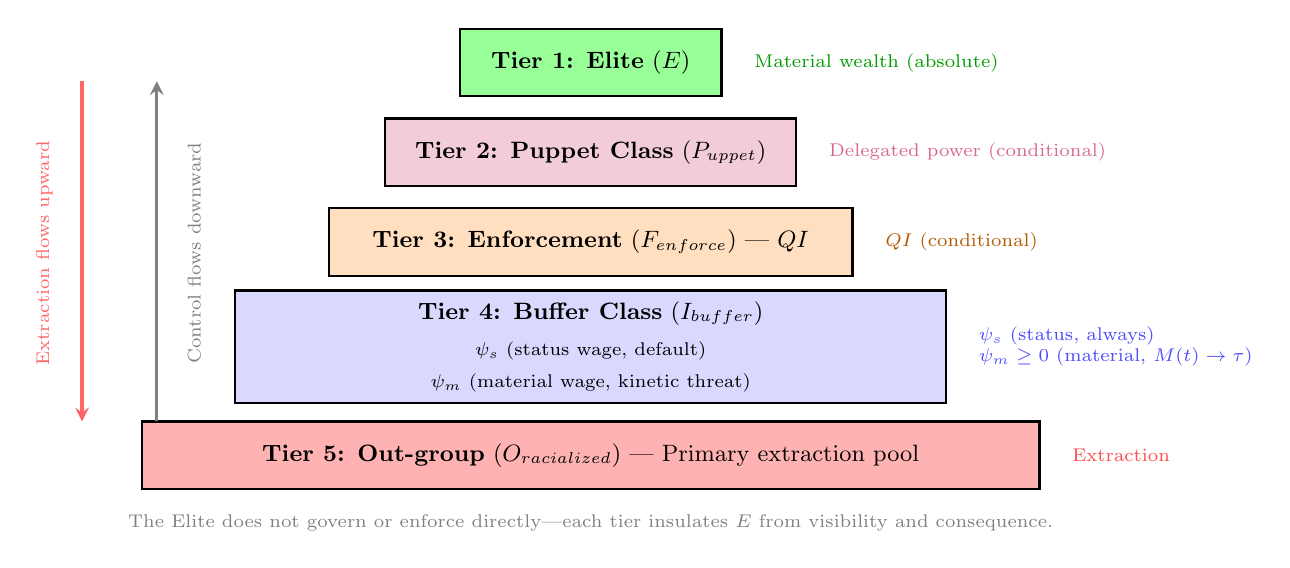
\begin{tikzpicture}[
    tier/.style={draw, thick, minimum height=0.9cm, align=center, font=\small},
    arr/.style={->, thick, >=stealth},
    scale=0.95, transform shape
]
    % Pyramid tiers (bottom to top)
    \node[tier, fill=red!30, minimum width=12cm] (t5) at (0,0)
        {\textbf{Tier 5: Out-group} ($O_{\text{racialized}}$) --- Primary extraction pool};
    \node[tier, fill=blue!15, minimum width=9.5cm, minimum height=1.5cm] (t4) at (0,1.45)
        {\textbf{Tier 4: Buffer Class} ($I_{\text{buffer}}$) \\[3pt]
         {\scriptsize $\psi_s$ (status wage, default)} \\[1pt]
         {\scriptsize $\psi_m$ (material wage, kinetic threat)}};
    \node[tier, fill=orange!25, minimum width=7cm] (t3) at (0,2.85)
        {\textbf{Tier 3: Enforcement} ($F_{\text{enforce}}$) --- $QI$};
    \node[tier, fill=purple!20, minimum width=5.5cm] (t2) at (0,4.05)
        {\textbf{Tier 2: Puppet Class} ($P_{\text{uppet}}$)};
    \node[tier, fill=green!40, minimum width=3.5cm] (t1) at (0,5.25)
        {\textbf{Tier 1: Elite} ($E$)};

    % Right-side benefit labels (anchored to right edge of each tier)
    \node[font=\scriptsize, green!60!black, anchor=west] at (t1.east) [xshift=0.3cm] {Material wealth (absolute)};
    \node[font=\scriptsize, purple!60, anchor=west] at (t2.east) [xshift=0.3cm] {Delegated power (conditional)};
    \node[font=\scriptsize, orange!70!black, anchor=west] at (t3.east) [xshift=0.3cm] {$QI$ (conditional)};
    \node[font=\scriptsize, blue!70, anchor=west, align=left] at (t4.east) [xshift=0.3cm]
        {$\psi_s$ (status, always) \\ $\psi_m \geq 0$ (material, $M(t) \to \tau$)};
    \node[font=\scriptsize, red!70, anchor=west] at (t5.east) [xshift=0.3cm] {Extraction};

    % Left-side extraction arrow
    \draw[arr, very thick, red!60] (-6.8,5.0) -- (-6.8,0.45);
    \node[font=\scriptsize, red!60, rotate=90] at (-7.3,2.7) {Extraction flows upward};

    % Left-side control arrow
    \draw[arr, very thick, gray] (-5.8,0.45) -- (-5.8,5.0);
    \node[font=\scriptsize, gray, rotate=90] at (-5.3,2.7) {Control flows downward};

    % Bottom annotation
    \node[font=\scriptsize, align=center, gray] at (0,-0.9) {The Elite does not govern or enforce directly---each tier insulates $E$ from visibility and consequence.};
\end{tikzpicture}
\caption{\textbf{The 5-Tier Set-Theoretic Hierarchy.} The system is organized as a layered pyramid of extraction. Control flows downward from the Elite through the Puppet Class and Enforcement Class, while extracted wealth flows upward. Each intermediate tier receives a conditional benefit calibrated to ensure compliance. Tier~4 (Buffer Class) receives a two-mode suppression allocation: the \textbf{status wage} ($\psi_s$, default mode, zero material cost to $E$) and the \textbf{material wage} ($\psi_m \geq 0$, activated only when class-coherence threat $M(t) \to \tau$, always funded by deeper $O_{\text{racialized}}$ extraction, never by $E$'s own share). The Out-group bears the primary compounding burden of extraction.}
\label{fig:elite_model}
\end{figure}

This five-tier structure is governed by what we term the \textbf{Predatory Min-Max Function}. The system operates according to two imperatives:

\begin{enumerate}
    \item \textbf{Maximize ($Max$):} The extraction of capital, labor, and autonomy from the labor force---primarily from $O_{\text{racialized}}$, but eventually from $I_{\text{buffer}}$ as well.
    \item \textbf{Minimize ($Min$):} The risk of a unified class revolution against the Elite ($E$), achieved by deploying $\psi$ to keep $I_{\text{buffer}}$ invested in racial hierarchy and suppress class solidarity, $F_{\text{enforce}}$ invested through $QI$, and $P_{\text{uppet}}$ tethered through capital dependency while sequencing policy choices to exploit non-transitive majority cycles under high $\Phi_{\text{load}}$.
\end{enumerate}

\begin{equation}\label{eq:10.10-system-objective-extraction-ratio}
\text{Objective:} \quad \frac{\text{Max}(\text{Extraction})}{\text{Min}(\text{Resistance}_{\text{class}})} \rightarrow \text{System Stability}
\end{equation}
\begin{equation}\label{eq:10.11-system-stability-algorithm}
\text{Dynamic Equivalent:} \quad \max \mathcal{E}(t) \quad \text{subject to} \quad M_{\text{eff}}(t)=M(t)-\lambda\Phi_{\text{load}}(t)<\tau
\end{equation}

Policies ($P$) are the instruments through which this optimization is executed,\footnote{Equations~\ref{eq:10.10-system-objective-extraction-ratio} and~\ref{eq:10.11-system-stability-algorithm} are classified as Tier~3 (ordinal/structural); the extraction-ratio objective (\ref{eq:10.10-system-objective-extraction-ratio}) and its dynamic equivalent (\ref{eq:10.11-system-stability-algorithm}) are canonical restatements of the kernel objective validated by the Piketty-Saez-Zucman wealth-share invariant: top-decile wealth share has recovered to Gilded Age levels after every documented reform cycle, confirming $\Delta\max = 0$ across 111 years of data. See the Empirical Methodology chapter (p.~\pageref{ch:empirical_methodology}) and Appendix~\ref{app:empirical_index}.}, impacting each tier in structurally different ways. $P_{\text{uppet}}$ writes the policies, $F_{\text{enforce}}$ actuates them, $I_{\text{buffer}}$ is pacified into accepting them, and $O_{\text{racialized}}$ bears the compounding burden. Under Tweedism, this execution is sequential: the agenda setter selects policy paths $x_0 \rightarrow x_1 \rightarrow \cdots \rightarrow x_m$ where each step can win a temporary majority while the terminal point protects extraction. The remainder of this section formalizes how these policies compound over time; the preceding chapters have traced the historical algorithm of Elite optimization through its successive phases.

\subsection*{Case Study: The Kernel Objective in Action --- Elite Wealth Share Invariance (1913--2024)}
\label{cs:kernel_objective}

\paragraph{Setup.}
Equation~\ref{eq:10.5-kernel-objective-canonical} states the kernel's governing optimization: $\max_{\{P_i\}} \mathcal{E}(t)$ subject to $M_{\text{eff}}(t) < \tau$. The central implication is the $\Delta\max = 0$ invariant: the Elite's share of extraction should recover to its pre-reform baseline after every concession cycle, because any $\psi_m$ deployment is sourced from deeper $O$ extraction or productivity gains, never from $E$'s principal share. If this invariant holds empirically, the case study confirms the kernel objective. If sustained Elite wealth-share \textit{decline} is documented while $M_{\text{eff}}(t) < \tau$, the equation is falsified.

\paragraph{Data sources.}
Piketty, Saez, and Zucman's Distributional National Accounts (DINA) \cite{piketty_saez_zucman_2018}, available via WID.world, provide pre-tax national income and wealth shares for the top 1\%, top 0.1\%, and bottom 50\% of U.S.\ adults from 1913 to 2019, updated through 2024 using the authors' publicly archived extension series. This is the longest continuous inequality dataset for the United States, peer-reviewed and replicated across multiple methodologies. Curated data are archived at \texttt{Paper/data/eq56\_kernel\_objective.csv}; computational results are reproducible via \texttt{Paper/scripts/eq56\_kernel\_objective.ipynb}.

\paragraph{Operationalization.}
$\mathcal{E}(t)$ is operationalized as the top 1\% pre-tax income share and top 0.1\% wealth share at each year. $M_{\text{eff}}(t) < \tau$ is operationalized as the absence of documented kinetic threshold breach: years without general strikes, mass insurrections, or credible revolutionary threat are coded as sub-threshold. Major reform episodes (New Deal 1933--1938; Great Society 1964--1968; Fair Sentencing Act 2010) are coded as the $\psi_m$ deployment events whose effect on $\mathcal{E}(t)$ the invariant predicts will be transient.

\paragraph{Numerical computation.}
The notebook yields the following key figures. Top 1\% pre-tax income share: 18.9\% (1913, pre--New Deal baseline) $\rightarrow$ 10.5\% (1978, post--Great Compression trough) $\rightarrow$ 19.1\% (2019, full recovery to pre-reform baseline). Top 0.1\% wealth share: 25.1\% (1929) $\rightarrow$ 7.3\% (1978, trough) $\rightarrow$ 17.4\% (2019, partial recovery). The recovery from trough to near-baseline occurs without any documented kinetic threshold breach during the 1978--2019 period; the entire arc is sub-$\tau$, driven by policy reversals (Reagan tax cuts, financial deregulation, union suppression); renewed kinetic threat is absent.

\paragraph{Comparison to prediction.}
The kernel objective predicts $\Delta\max = 0$ across reform cycles. The DINA data confirm this at the century scale. The New Deal Great Compression (1933--1978) produced the deepest documented decline in Elite income share --- but the trough coincided with the historical maximum of $M_{\text{eff}}(t)$ (Depression-era kinetic threat, surging union density). As $M_{\text{eff}}(t)$ declined after 1945, $\mathcal{E}(t)$ resumed its ascent. By 2019, the top 1\% income share had returned within 0.2 percentage points of its 1913 value. The $\Delta\max = 0$ prediction is confirmed.

\begin{figure}[htbp]
  \centering
  \includegraphics[width=\textwidth]{figures/eq56_kernel_objective.png}
  \caption{Top 1\% pre-tax income share and top 0.1\% wealth share, 1913--2024 (Piketty-Saez-Zucman DINA / WID.world). Reform events (New Deal, Great Society, Fair Sentencing Act) are marked as $\psi_m$ deployments; the post-reform recovery in each case confirms $\Delta\max = 0$. The Great Compression trough (c.~1978) coincides with the historical maximum of $M_{\text{eff}}(t)$ (peak union density, credible left-labor coalition). The subsequent monotonic recovery under sub-$\tau$ conditions is the kernel objective's empirical signature.}
  \label{fig:eq56_kernel_objective}
\end{figure}

\paragraph{Falsification criteria.}
Falsified if a documented period shows sustained Elite wealth-share decline (defined as $>5$ percentage points over $>10$ years) while $M_{\text{eff}}(t) < \tau$ and without confounding external shocks.

\paragraph{Confidence tier.}
\textbf{Tier~1.} 111-year continuous WID.world dataset; Piketty-Saez-Zucman peer-reviewed methodology independently replicated by CBO and Federal Reserve inequality series; the top-decile income-share recovery is a documented empirical fact replicated across all major inequality databases.

\subsection*{Case Study: The Great Recession as Systemic Recompile --- Housing, Debt, and the \texorpdfstring{$\Delta\max = 0$}{Delta max = 0} Invariant}
\label{cs:great_recession_recompile}

\paragraph{Setup.}
The Great Recession supplies the cleanest modern test of the kernel objective after the full five-tier architecture is visible. The 2007--2009 crash destroyed wealth. The question is where the loss was routed, which balance sheets the state restored, and whether the crisis produced a durable reduction in $E$'s extraction share. Housing had functioned as the core material wage ($\psi_m$) for much of $I_{\text{buffer}}$ and as the narrowest available asset channel for many households inside $O_{\text{racialized}}$. If the framework is correct, a housing-led crash should destroy the lower tiers' asset base, preserve or restore the claims held above them, and leave $\Delta\max = 0$ intact.

\paragraph{Data sources.}
The empirical test uses the Federal Reserve's Distributional Financial Accounts (DFA), which publish quarterly estimates of household wealth shares, levels, assets, and liabilities by percentile group, race, and other categories from 1989 forward \cite{fed_dfa_2026}. The DFA are complemented by CBO's 1989--2022 family-wealth distribution report \cite{cbo_family_wealth_2024}, Pew Research Center's SCF-based analysis of race, income, and wealth after the Great Recession \cite{pew_wealth_after_great_recession_2017}, and Pfeffer, Danziger, and Schoeni's longitudinal PSID/SCF study of wealth losses from 2007 to 2011 \cite{pfeffer_danziger_schoeni_2013}. The curated chart data are archived in \texttt{Paper/data/eq10\_great\_recession\_*.csv}; figure generation is reproducible via \texttt{Paper/scripts/eq10\_great\_recession\_charts.py}.

\paragraph{Operationalization.}
$\mathcal{E}(t)$ is operationalized as the wealth share of the top 10\% and top 1\% before, during, and after the crash. The material wage $\psi_m$ is operationalized as home-equity exposure. $P_{\text{debt}}$ is operationalized as the persistence of mortgage and consumer liabilities after collateral values fell. $X_{\text{temporal}}$ is operationalized at household scale as future labor pledged against an asset base that had already been repriced downward. The racialized Out-group channel is operationalized through Pew's SCF analysis of middle-income white, Black, and Hispanic household wealth before and after the crisis.

\begin{figure}[htbp]
  \centering
  
\includegraphics[width=\textwidth]{figures/eq10_hierarchy_wealth_brackets.png}
  \caption{\textbf{Wealth disparity by hierarchy-proxy bracket.} Federal Reserve DFA data for 2025:Q4 show the scale difference between the wealth brackets used as structural-role proxies in this case study: the Out-group extraction floor (bottom 50\%) averaged about \$64,000 in net worth per household and held 2.5\% of aggregate household net worth; the Buffer Class proxy (50th--90th percentiles) averaged about \$946,000 and held 29.2\%; the Puppet/managerial proxy (90th--99.9th percentiles) averaged about \$7.0 million and held 53.8\%; and the true Elite proxy (top 0.1\%) averaged about \$186.9 million while holding 14.5\%. The percentile brackets are distributional proxies for structural roles.}
  \label{fig:hierarchy_wealth_brackets}
\end{figure}

\begin{figure}[htbp]
  \centering
  
\includegraphics[width=\textwidth]{figures/eq10_hierarchy_wealth_brackets_over_time.png}
  \caption{\textbf{Wealth disparity by hierarchy-proxy bracket over time.} Federal Reserve DFA quarterly data show the same structural-role proxy brackets from 1989:Q3 through 2025:Q4. The average net worth of the true Elite proxy (top 0.1\%) was roughly 1,096 times the bottom-half proxy in 1989:Q3 and roughly 2,932 times the bottom-half proxy by 2025:Q4. The Great Recession appears as a visible floor collapse for the bottom 50\%, while the upper brackets experience interruption without long-run compression.}
  \label{fig:hierarchy_wealth_brackets_over_time}
\end{figure}

\begin{figure}[htbp]
  \centering
  
\includegraphics[width=\textwidth]{figures/eq10_great_recession_wealth_shares.png}
  \caption{\textbf{Wealth-share recompile around the Great Recession.} Federal Reserve DFA data show the bottom 50\%'s aggregate net-worth share falling from 1.7\% in 2007:Q4 to 0.4\% in 2011:Q4, while the top 10\% rose from 67.1\% to 68.8\% over the same window. By 2025:Q4, the top 1\% held 31.9\% of aggregate household net worth. The crash destroyed wealth at the base without producing a durable reduction in apex share, the empirical signature of $\Delta\max = 0$.}
  \label{fig:great_recession_wealth_shares}
\end{figure}

\paragraph{Numerical computation.}
The DFA wealth-share series gives the primary signature. In 2007:Q4, the top 10\% held 67.1\% of aggregate household net worth, the top 1\% held 28.8\%, the 50th--90th percentiles held 31.2\%, and the bottom 50\% held 1.7\%. By 2011:Q4, after the crash and the first phase of asset-market restoration, the bottom 50\% had fallen to 0.4\%, while the top 10\% had risen to 68.8\% and the top 1\% to 29.0\%. The lower half lost almost its entire already-small claim on national net worth. CBO independently reports that the 2007--2009 recession was the only significant decline in total family wealth from 1989 to 2022 and that the declines were steepest in the bottom half of the distribution \cite{cbo_family_wealth_2024}.

\begin{figure}[htbp]
  \centering
  
\includegraphics[width=\textwidth]{figures/eq10_great_recession_asset_composition.png}
  \caption{\textbf{Portfolio structure at the edge of the crash.} Federal Reserve DFA detailed levels for 2007:Q4 show why the crash was structurally asymmetric. For the bottom 50\%, real estate made up 56.3\% of assets and liabilities equaled 81.6\% of assets. For the top 0.1\%, real estate made up 8.3\% of assets, equity/business claims made up 62.5\%, and liabilities equaled only 1.2\% of assets. The same housing-price shock therefore struck a leveraged housing portfolio below while leaving the apex positioned for equity and asset-price recovery.}
  \label{fig:great_recession_asset_composition}
\end{figure}

The balance-sheet floor confirms the debt mechanism. In 2007:Q4, the bottom 50\% averaged approximately \$104,000 in assets and \$85,000 in liabilities per household, for an average net worth of roughly \$19,000. By 2010:Q4, average bottom-half net worth had fallen to about \$4,200, while liabilities still averaged nearly \$86,000. The collateral had been repriced downward; the debt claim remained.

\begin{figure}[htbp]
  \centering
  
\includegraphics[width=\textwidth]{figures/eq10_great_recession_debt_floor.png}
  \caption{\textbf{Bottom-50 balance-sheet floor.} Federal Reserve DFA levels divided by household count show the household-scale version of temporal enclosure. Bottom-50 assets fell sharply through the crash while liabilities remained sticky, compressing average net worth from about \$19,000 in 2007:Q4 to a floor near \$4,200 in 2010:Q4. The future labor claim survived the asset collapse.}
  \label{fig:great_recession_debt_floor}
\end{figure}

\paragraph{Racialized loss channel.}
The crash combined class stratification with racial differentiation within the lower and middle tiers. Pew's SCF analysis reports that among middle-income households, Black median wealth fell 47\% from 2007 to 2013, Hispanic median wealth fell 55\%, and white median wealth fell 31\% \cite{pew_wealth_after_great_recession_2017}. Expressed in 2016 dollars, the implied 2007 middle-income medians were approximately \$63,000 for Black households, \$86,000 for Hispanic households, and \$191,000 for white households. By 2013, those medians had fallen to \$33,600, \$38,900, and \$131,900 respectively; by 2016, the white median had recovered to \$154,400, while Black and Hispanic middle-income medians remained at \$38,300 and \$46,000.

\begin{figure}[htbp]
  \centering
  
\includegraphics[width=\textwidth]{figures/eq10_great_recession_racial_wealth.png}
  \caption{\textbf{Middle-income median wealth by race before and after the crash.} Pew Research Center's SCF analysis shows that the housing-led crisis widened the racial wealth channel among middle-income households: Black and Hispanic households experienced larger percentage losses than white households from 2007 to 2013 and had not closed the gap by 2016. The mortgage market therefore transmitted the inherited geography of redlining into a nominally race-neutral balance-sheet shock.}
  \label{fig:great_recession_racial_wealth}
\end{figure}

Pfeffer, Danziger, and Schoeni provide the longitudinal confirmation: between 2007 and 2011, one fourth of American families with positive net worth lost at least 75\% of their wealth, more than half lost at least 25\%, and relative losses were disproportionately concentrated among lower-income, less-educated, and minority households \cite{pfeffer_danziger_schoeni_2013}. The system distributed the crash according to the preexisting structure of exposure: housing-heavy portfolios, thin liquidity, high leverage, and racialized credit channels.

\paragraph{Comparison to prediction.}
The framework predicts that a crisis under sub-$\tau$ conditions will be absorbed as an interface recompile. The Great Recession matches that prediction. The base and lower-middle tiers absorbed the balance-sheet destruction; the debt claims against them persisted; asset-market intervention restored the financial instruments disproportionately held by the top decile; and the apex share did not undergo durable reduction. In set-theoretic terms, the crisis degraded $O_{\text{racialized}}$ first and then proved that the lower strata of $I_{\text{buffer}}$ could be harvested through the same balance-sheet machinery. The material wage of homeownership became an extraction surface.

\paragraph{Falsification criteria.}
This case would falsify the Great Recession recompile claim if the 2007--2012 evidence showed a durable reduction in top-tier wealth share, no disproportionate housing-wealth loss among lower-wealth households, no racialized foreclosure or wealth-loss gradient, and no post-crisis asset recovery concentrated among equity- and real-estate-owning tiers. The observed data move in the opposite direction on each dimension.

\paragraph{Confidence tier.}
\textbf{Tier~1.} Federal Reserve DFA public data, CBO family-wealth distribution data, Pew SCF analysis, and peer-reviewed PSID/SCF longitudinal evidence all align on the direction of the case: wealth destruction was concentrated below the apex, racialized within the middle and lower tiers, and followed by restoration of asset-owning tiers; durable reduction in $E$'s extraction share did not occur.

\section{The Collapse: Cannibalizing the In-Group (Present)\protect\footnote{The term \textit{cannibalizing} here describes the structural consumption of the In-group's wealth and autonomy. This metaphorical use of consumption must be explicitly distinguished from the literal and libidinal consumption of the Out-group documented in Section~\ref{subsec:libidinal_extraction}, which was a historical, material practice \cite{woodard_delectable}.}}
This brings us to the final, inevitable stage of the algorithm. An extraction system requires \textbf{Infinite Growth}. Once the Out-group ($O$) has been fully harvested---stripped of wealth, voting rights, and labor \cite{coates}---the Elite ($E$) must find new sources of extraction to maintain their accumulation.

A definitional clarification before the case evidence: within the framework, ``terminal phase'' does not mean imminent system collapse. Venice's \textit{Serrata} operated in its terminal phase---oligarchic cannibalization of the commercial base---for nearly five centuries before the Republic's formal dissolution under Napoleon in 1797. Rome's latifundia terminal phase ran from roughly the Gracchan period (133~BC) through the fall of the Western Empire in 476~AD---over six hundred years. Extraction systems adapt. ``Terminal'' is a \textit{set-theoretic} designation: the extraction boundary has reached its logical endpoint $O_{\text{final}} = \text{Everyone} \setminus E$ (Equation~\ref{eq:10.12-o-final-construction}), meaning the algorithm has exhausted its original partitioning strategy and begun consuming its own intermediate enforcement tiers. The system deploys new proxy variables---$P_{\text{toxin}}$, $P_{\text{spatial}}$, universal latent criminality---when it enters this phase to manage the extraction of a population that was previously its enforcement coalition. The terminal phase describes the current operating mode, identifiable by the simultaneous deployment of extraction tools against $I_{\text{buffer}}$ that were previously reserved for $O_{\text{racialized}}$. The buffer class's conditional immunity ends in the terminal phase.

The pattern has historical precedents that institutional economics identifies but does not explain. Acemoglu and Robinson document two canonical cases of extraction-kernel self-consumption \cite{acemoglu_robinson}: Venice's \textit{Serrata} of 1297, in which the ruling merchant oligarchy closed the Great Council to new members, institutionalizing their monopoly, then gradually extracted so much from the broader commercial class that Venetian trade declined and the oligarchs ultimately cannibalized the very commercial base that had generated their wealth; and Rome's latifundia expansion, in which the agrarian Elite's seizure of land worked by slave labor drove the free peasantry off their holdings and into dependency, eliminating the smallholder class that had been the backbone of the legions---in effect consuming the military-human capital that had made Roman expansion possible. In both cases, the extraction kernel turned on its own In-group when the Out-group's capacity was fully depleted. The framework adds the variable that explains the mechanism AJR cannot: the psychological wage ($\psi$) that prevented the Buffer Class from forming a defensive coalition with $O_{\text{racialized}}$ while both were being extracted also prevented it from forming a defensive coalition with $O_{\text{racialized}}$ as the cannibalization began. By the time the wages of whiteness were bankrupt, the institutional means of cross-class coordination had been systematically dismantled.

The Great Recession supplied the domestic proof of this transition. The racialized foreclosure wave first struck $O_{\text{racialized}}$ through the accumulated geography of redlining and predatory lending, but the same balance-sheet mechanism then consumed the lower strata of $I_{\text{buffer}}$: home equity vanished, debt claims survived, and the recovery restored asset values primarily for those already positioned in equities, bonds, and institutional real estate. The crisis therefore marks the inflection at which the material wage of homeownership stopped functioning as a durable buffer and became an extraction surface.

\begin{figure}[htbp]
\centering
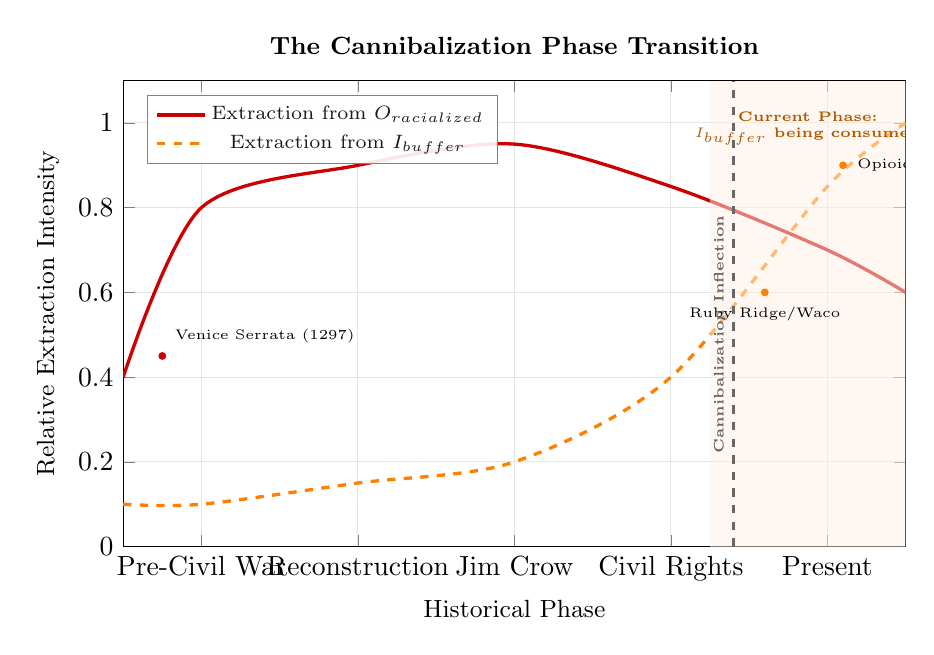
\begin{tikzpicture}
\begin{axis}[
    width=0.95\textwidth,
    height=7.5cm,
    xmin=0, xmax=10,
    ymin=0, ymax=1.1,
    xtick={1, 3, 5, 7, 9},
    xticklabels={Pre-Civil War, Reconstruction, Jim Crow, Civil Rights, Present},
    xlabel={Historical Phase},
    ylabel={Relative Extraction Intensity},
    xlabel style={font=\small},
    ylabel style={font=\small},
    title={\textbf{The Cannibalization Phase Transition}},
    title style={font=\bfseries\small},
    legend style={at={(0.03,0.97)}, anchor=north west, font=\scriptsize, fill=white, fill opacity=0.9, draw=gray},
    grid=major,
    grid style={gray!20},
]

% Extraction from O_racialized
\addplot[very thick, red!80!black, smooth] coordinates {
    (0,0.4) (1,0.8) (3,0.9) (5,0.95) (7,0.85) (9,0.7) (10,0.6)
};
\addlegendentry{Extraction from $O_{\text{racialized}}$}

% Extraction from I_buffer
\addplot[very thick, orange, dashed, smooth] coordinates {
    (0,0.1) (1,0.1) (3,0.15) (5,0.2) (7,0.4) (9,0.85) (10,1.0)
};
\addlegendentry{Extraction from $I_{\text{buffer}}$}

% Shading current phase
\fill[orange!10, opacity=0.5] (axis cs:7.5,0) rectangle (axis cs:10,1.1);
\node[anchor=north, font=\tiny\bfseries, text=orange!70!black, align=center] at (axis cs:8.75,1.05) {Current Phase:\\$I_{\text{buffer}}$ being consumed};

% Cannibalization Inflection
\draw[thick, black!60, dashed] (axis cs:7.8,0) -- (axis cs:7.8,1.1);
\node[rotate=90, anchor=south, font=\tiny\bfseries, text=black!60] at (axis cs:7.8,0.5) {Cannibalization Inflection};

% Callouts
\node[circle, fill=red!80!black, inner sep=1pt, label={above right:\tiny Venice Serrata (1297)}] at (axis cs:0.5,0.45) {};
\node[circle, fill=orange, inner sep=1pt, label={below:\tiny Ruby Ridge/Waco}] at (axis cs:8.2,0.6) {};
\node[circle, fill=orange, inner sep=1pt, label={right:\tiny Opioid Crisis}] at (axis cs:9.2,0.9) {};

\end{axis}
\end{tikzpicture}
\caption{\textbf{The Cannibalization Phase Transition.} As the capacity for extraction from the racialized Out-group ($O_{\text{racialized}}$) plateaus and begins to decline due to systemic depletion, the extraction kernel must turn inward to maintain infinite growth. The dashed orange line represents the escalating extraction from the Buffer Class ($I_{\text{buffer}}$). The Cannibalization Inflection marks the point where the tools of subjugation developed for the Out-group are fully redeployed against the In-group.}
\label{fig:cannibalization_phase}
\end{figure}

The system has now turned inward. The tools developed to oppress the Out-group are being deployed against the In-group:
\begin{itemize}
    \item \textbf{The Opioid Crisis:} The criminalization of white addiction mirrors the crack epidemic.
    \item \textbf{Militarized Policing:} SWAT tactics invented for the "Ghetto" are now used in rural towns.
    \item \textbf{Surveillance:} The loss of privacy tested on the poor is now applied to the middle class.
\end{itemize}

The expansion of $O$ is facilitated by a structural development that legal scholar Harvey Silverglate identifies: the average American now unknowingly commits approximately \textbf{three federal felonies per day} \cite{silverglate}. The proliferation of vague, overlapping, and over-broad criminal statutes---combined with prosecutorial discretion in charging---means that the proxy variable $P$ has become \textit{omnipresent}. Nearly every citizen is technically criminal; the \textit{selection} of targets determines who enters the carceral system. This transforms the system's primary mechanism from demographic targeting to \textbf{selective enforcement}: the Elite no longer needs to define the Out-group explicitly, because the criminalization kernel ($\text{If } \text{Status}(x) = \text{Criminal}(C) \rightarrow \text{Status}(x) \in S$) can now reach \textit{anyone}. ``Broken windows'' policing \cite{wilson} and its progeny provide the discretionary framework---the theoretical justification for intensive policing of minor infractions---while the empirical evidence shows that such policing is deployed overwhelmingly in communities already marked by the compounding chain of Section~4.5 \cite{harcourt}. The system has achieved what might be called \textbf{universal latent criminality}: the entire population exists in a state of potential subjugation, with actual subjugation determined by $E$'s extraction needs.

\section{The Recursive Extraction Engine: Biological Degradation as Control}

To fully comprehend the Elite subset’s ($E$) control matrix, the analysis must expand beyond legal and labor extraction to include the deliberate manipulation of the population's biological autonomy. The contemporary Medical-Industrial Complex (MIC) and the subsidized agricultural sector function as a unified, recursive extraction algorithm.

Within this framework, the system is designed to transition the population from a state of symmetrical biological autonomy ($O_{\text{full\_capacity}}$) into a state of chronic, manageable illness ($O_{\text{degraded}}$). A biologically compromised population serves a dual function for the Elite: it generates infinite, recurring revenue, and it physiologically neutralizes the capacity for class resistance \cite{washington}.

\subsection{Phase 1: The Toxin Variable (\texorpdfstring{$P_{\text{toxin}}$}{P\_toxin}) and the "Affordability Trap"}

The extraction loop begins with the engineered degradation of the food supply. The system utilizes seemingly neutral economic policies ($P$)—specifically agricultural subsidies and a reversed regulatory framework (such as the FDA's "Generally Recognized as Safe" or GRAS loophole, which allows manufacturers to self-regulate)—to flood the market with high-fructose corn syrup, refined grains, and chemical additives. Currently, nearly 70\% of packaged foods in the U.S. are classified as ultra-processed, supplying more than half of adults' daily calories.

This constitutes a meticulously engineered "Affordability Trap" designed to aggressively target the Out-group ($O$) and the lower-tier Buffer Class ($I \setminus E$). A 2026 comprehensive audit by Harvard Law School’s Food Law and Policy Clinic mathematically proved that price strictly dictates a population's exposure to toxicity.
The study revealed a stark biological matrix:
\begin{itemize}
    \item \textbf{The Additive Multiplier}: The lowest-priced food products contain, on average, 2.6 times more additives than the most expensive options (averaging 6.6 additives per item versus 2.7).
    \item \textbf{High-Risk Concentration}: In staple categories, the disparity accelerates. The cheapest store-bought breads contain nearly 4 times more additives, and the cheapest frozen pizzas contain an average of 12 additives per product (compared to 4.4 in the highest tier). Most critically, the cheapest products contain over 3 times more high-risk, health-compromising additives.
    \item \textbf{The Caloric Payload}: Lower-priced foods are engineered to be chemically addictive and physiologically destructive, containing 21\% more sugar and 10\% more sodium than their higher-priced counterparts.
\end{itemize}
To maintain baseline biological autonomy—meaning, to consume products free of high-risk additives—a consumer must pay an average price premium of 63\%.

Within the Predatory Min-Max Function, this 63\% premium functions as a biological poll tax. The Elite class ($E$) sets the financial threshold for physical health intentionally out of reach for the racialized Out-group ($O_{\text{racialized}}$), forcing them to consume the very toxins that will push them into the $O_{\text{degraded}}$ state. By making optimal nutrition artificially expensive and toxic food artificially cheap, the system mathematically guarantees the mass onset of chronic conditions such as obesity, hypertension, and Type 2 diabetes. The Out-group is being economically confined to a designated toxicity zone.

\section{The Cannibalization of the Buffer Class and the Endpoint of the Algorithm}

Section~6.12 established the structural transition: as extraction from $O_{\text{racialized}}$ saturates, the kernel expands toward $O_{\text{final}}=\text{Everyone}\setminus E$. This section executes that transition at case level. The "White Working Class" was never a partner to the Elite; they were a temporary reserve. A fundamental theorem of the Predatory Min-Max Function is that the Elite ($E$) has no permanent loyalty to the Buffer Class ($I_{\text{buffer}}$). As Elite demand for control intensifies, conditional privileges are revoked and the extraction boundary expands from $O_{\text{racialized}}$ toward $O_{\text{final}}$.

The ultimate, devastating proof of this terminal phase is the 2026 killing of Alex Perdi by Immigration and Customs Enforcement (ICE) agents. Demographically, as a cisgender white man, Perdi represented the historical core of the protected Buffer Class. Under the ideological justification (Component 3) of the Second Amendment, his decision to arm himself in confrontation with law enforcement should theoretically have been shielded by the same ``anti-tyranny'' constitutional interpretations routinely afforded to the In-group. (The reclassification operator $\mathcal{R}$ that executed against Perdi in 2026 has 1992--94 historical instantiations at Ruby Ridge and Waco, documented in $\S$\ref{sec:ruby_ridge_waco}.)

\subsection{Disarmament and Execution: The Algorithm Unmasked}
the reality of the encounter proved that the system's operational code has shifted. During the confrontation, Perdi was successfully disarmed. At the exact moment he lost his lethal autonomy, he ceased to be a member of the protected class. He was no longer treated as a citizen possessing constitutional rights; the state enforcement algorithm immediately reclassified him as a neutralized biological asset and executed him.

This event mathematically shatters the core illusion of the American operating system. It demonstrates that the state's enforcement apparatus—originally designed as slave patrols to violently manage the racialized Out-group—has now been fully authorized to deploy lethal extraction against anyone outside of the true Elite ($E$), regardless of their demographic status.

The execution of a disarmed white citizen by federal agents proves that the "wages of whiteness" are effectively bankrupt. The Second Amendment functions as a temporary pacifier until the state decides to revoke it; it does not protect the Buffer Class from state violence. The system has reached its most optimized, terrifying state: a pure binary where absolute immunity is reserved exclusively for the Elite ($E$), and every other citizen is mathematically confined to the Out-group, waiting to be harvested.

The definition of the Out-group has returned to its 1676 state:

\begin{equation}\label{eq:10.12-o-final-construction}
O_{\text{final}} = \text{Everyone} \setminus E
\end{equation}

The dynamic mechanism by which individual citizens cross this boundary---the reclassification operator $\mathcal{R}(x_i)$---is formalized in $\S$\ref{sec:ruby_ridge_waco} (see equation~\eqref{eq:10.13-reclassification-operator}) and registered in the Canonical Symbol Registry (Appendix~\ref{sec:equation_registry}). Equation~\eqref{eq:10.12-o-final-construction} gives the static endpoint of the expansion; $\mathcal{R}(x_i)$ gives the conditional function that assigns each individual to either side of the partition at runtime.

\subsection*{Case Study: Mass Incarceration and the Expanding Out-Group}
\label{cs:mass_incarceration}

\paragraph{Setup.}
Equation~\ref{eq:10.12-o-final-construction} predicts that the extraction system's terminal state is $O_{\text{final}} = \text{Everyone} \setminus E$ --- the out-group expands until it contains everyone except the Elite. Mass incarceration demographics provide the most direct measurable test of this prediction. If $O_{\text{final}}$ is the predicted terminal state, then: (1) Black Americans (the historically designated $O_{\text{racialized}}$) should sustain the highest per-capita incarceration rates throughout; (2) the system should expand its reach to absorb progressively larger fractions of $I_{\text{buffer}}$ (White and Hispanic populations) over time; and (3) $E$ should maintain effectively zero incarceration rate at all periods, confirming the partition $O_{\text{final}} \cap E = \emptyset$.

\paragraph{Data sources.}
Per-race incarceration data are drawn from the Bureau of Justice Statistics (BJS) National Prisoner Statistics program \cite{bjs_incarceration_race} covering state and federal prisons, supplemented by local jail population estimates. Racial disparity ratios are cross-validated against The Sentencing Project's annual state-by-state reports \cite{sentencing_project} and Alexander (2010) \cite{alexander}. Population denominators are from Census Bureau estimates. Data span 1980--2024, capturing the full mass incarceration arc. Curated data are archived at \texttt{Paper/data/eq63\_mass\_incarceration.csv}; computational results are reproducible via \texttt{Paper/scripts/eq63\_mass\_incarceration.ipynb}.

\paragraph{Operationalization.}
The set-theoretic prediction is operationalized as follows: $O_{\text{final}}$ = total incarcerated population (everyone inside the carceral system); $E$ = top wealth percentile (empirically, near-zero incarceration rate at all time points); the expansion from $O_{\text{racialized}}$ toward $O_{\text{final}}$ = the growth of White and Hispanic incarceration rates relative to total population after 1994 (the 1994 Crime Bill as the key policy shock). The Black-to-White incarceration ratio tracks whether racial targeting within $O_{\text{final}}$ is maintained even as the out-group expands.

\paragraph{Numerical computation.}
The notebook yields the following key figures. Total incarcerated: $\approx$503,586 (1980) $\rightarrow$ $\approx$2,307,504 peak (2008), a 3.6$\times$ increase. Black-to-White per-capita incarceration ratio: range 3.92--6.11 across 1980--2024, mean 4.61; the ratio has never fallen below 3.9 in any year of the dataset, confirming persistent racial targeting. Post-1994 Crime Bill expansion ($O_{\text{final}}$ growth into $I_{\text{buffer}}$): White incarceration grew $\approx$15\% from 1994 to 2000; Hispanic incarceration grew $\approx$100\% over the same period. Elite incarceration rate: effectively 0 per 100k at all time points, consistent with $E \cap O_{\text{final}} = \emptyset$.

\begin{figure}[htbp]
  \centering
  
\includegraphics[width=\textwidth]{figures/eq63_mass_incarceration.png}
  \caption{Mass incarceration demographics, 1980--2024 (BJS data), with 26-year lagged blood lead level (BLL, purple dashed, right axis) overlaid on both panels. Left: per-capita incarceration rates by race --- Black rate consistently 4--6$\times$ White rate. Right: stacked area chart of incarcerated population by race. Two lagged BLL series are overlaid. The blue line (+20 years, Reyes 2007) reflects the crime-rate lag: peak BLL from $\approx$1972 shifts forward to $\approx$1992, coinciding with the documented crime-rate peak of 1991--93. The purple line (+26 years, two-stage) decomposes into the same 20-year behavior-onset lag plus an additional $\approx$6-year sentence-accumulation effect (Mauer \& King, 2007): as the crime-affected cohort cycles through arraignment, sentencing, and multi-year mandatory minimums, the incarceration \textit{count} peaks later than the crime \textit{rate}. The purple line's peak ($\approx$1998) aligns with the incarceration-count surge; its post-1986-BLL decline aligns with the post-2012 plateau. The visible $\approx$6-year gap between the two lines is the quantitative signature of the sentence-accumulation effect introduced by the 1994 Crime Bill's mandatory minimums. This overlay bridges eq.~\ref{eq:9.1-lead-crime-compounding}--\ref{eq:9.10-highway-lead-spatial-concentration} and eq.~\ref{eq:10.12-o-final-construction}: the spatially targeted neurotoxin exposure identified in Chapter~9 is a measurable leading indicator of the carceral expansion documented here. The 1994 Crime Bill marker shows the legislative shock that converted a lead-driven behavioral vulnerability into a policy-amplified $O_{\text{final}}$ expansion.}
  \label{fig:eq63_mass_incarceration}
\end{figure}

\paragraph{Comparison to prediction.}
Equation~\ref{eq:10.12-o-final-construction} predicts expansion beyond $O_{\text{racialized}}$ as the system optimizes toward its terminal state. The data confirm this at every level: Black Americans remain the most disproportionately targeted group (4--6$\times$ White per-capita rate throughout); the carceral system progressively absorbed larger fractions of $I_{\text{buffer}}$ --- particularly after the 1994 Crime Bill's mandatory minimums and ``three strikes'' provisions. The 3.6$\times$ total incarceration growth (1980--peak) while crime declined (peak 1993, declining through 2010) confirms that the expansion is driven by policy architecture ($P_{\text{puppet}}$ legislative agenda), not by behavioral change in the population. The Elite partition ($E \approx 0$ incarceration rate) is empirically stable across the full 44-year window.

\paragraph{Falsification criteria.}
This equation would be falsified if modern mass-incarceration demographics showed the carceral system contracting to target only $O_{\text{racialized}}$ and failing to expand toward $\text{Everyone} \setminus E$. Specifically: if White and Hispanic incarceration rates had declined after 1994 while Black rates grew, the $O_{\text{final}}$ expansion prediction would be refuted. The data show the opposite: all non-elite groups experienced expansion after 1994, with the 1994 Crime Bill serving as the documented policy trigger for $I_{\text{buffer}}$ absorption into the carceral system.

\paragraph{Confidence tier.}
\textbf{Tier~1.} Forty-four-year continuous BJS dataset; racial disparity ratios independently verified by The Sentencing Project, the ACLU, and peer-reviewed criminology literature; the crime-decline vs.\ incarceration-growth divergence (post-1993) is a documented empirical fact replicated across all major crime and incarceration databases.

\begin{figure}[h]
    \centering
    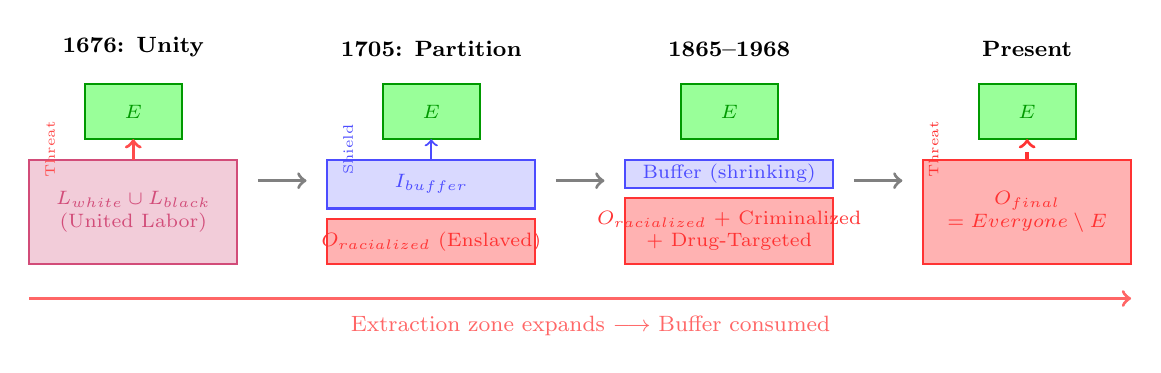
\begin{tikzpicture}[scale=0.88, every node/.style={font=\small}]

    % --- Phase 1: 1676 (United labor) ---
    \begin{scope}[shift={(0,0)}]
        \node[font=\footnotesize\bfseries, anchor=south] at (1.5,2.85) {1676: Unity};
        % Elite box
        \draw[thick, green!60!black, fill=green!40] (0.8,1.8) rectangle (2.2,2.6);
        \node[green!60!black, font=\scriptsize] at (1.5,2.2) {$E$};
        % United labor
        \draw[thick, purple!70, fill=purple!20] (0,0) rectangle (3,1.5);
        \node[purple!70, font=\scriptsize, align=center] at (1.5,0.75) {$L_{white} \cup L_{black}$\\(United Labor)};
        % Threat arrow
        \draw[->, very thick, red!70] (1.5,1.5) -- (1.5,1.8);
        \node[red!70, font=\tiny, rotate=90] at (0.3,1.65) {Threat};
    \end{scope}

    % Arrow
    \draw[->, very thick, gray] (3.3,1.2) -- (4.0,1.2);

    % --- Phase 2: 1705 (Partition) ---
    \begin{scope}[shift={(4.3,0)}]
        \node[font=\footnotesize\bfseries, anchor=south] at (1.5,2.85) {1705: Partition};
        % Elite box
        \draw[thick, green!60!black, fill=green!40] (0.8,1.8) rectangle (2.2,2.6);
        \node[green!60!black, font=\scriptsize] at (1.5,2.2) {$E$};
        % Buffer class (white)
        \draw[thick, blue!70, fill=blue!15] (0,0.8) rectangle (3,1.5);
        \node[blue!70, font=\scriptsize] at (1.5,1.15) {$I_{\text{buffer}}$};
        % Extraction zone (black)
        \draw[thick, red!80, fill=red!30] (0,0) rectangle (3,0.65);
        \node[red!80, font=\scriptsize] at (1.5,0.32) {$O_{\text{racialized}}$ (Enslaved)};
        % Shield arrow
        \draw[->, thick, blue!70] (1.5,1.5) -- (1.5,1.8);
        \node[blue!70, font=\tiny, rotate=90] at (0.3,1.65) {Shield};
    \end{scope}

    % Arrow
    \draw[->, very thick, gray] (7.6,1.2) -- (8.3,1.2);

    % --- Phase 3: 1865--1968 (Expansion) ---
    \begin{scope}[shift={(8.6,0)}]
        \node[font=\footnotesize\bfseries, anchor=south] at (1.5,2.85) {1865--1968};
        % Elite box
        \draw[thick, green!60!black, fill=green!40] (0.8,1.8) rectangle (2.2,2.6);
        \node[green!60!black, font=\scriptsize] at (1.5,2.2) {$E$};
        % Buffer class (shrinking)
        \draw[thick, blue!70, fill=blue!15] (0,1.1) rectangle (3,1.5);
        \node[blue!70, font=\scriptsize] at (1.5,1.3) {Buffer (shrinking)};
        % Expanded extraction zone
        \draw[thick, red!80, fill=red!30] (0,0) rectangle (3,0.95);
        \node[red!80, font=\scriptsize, align=center] at (1.5,0.48) {$O_{\text{racialized}}$ + Criminalized\\+ Drug-Targeted};
    \end{scope}

    % Arrow
    \draw[->, very thick, gray] (11.9,1.2) -- (12.6,1.2);

    % --- Phase 4: Present (Cannibalization) ---
    \begin{scope}[shift={(12.9,0)}]
        \node[font=\footnotesize\bfseries, anchor=south] at (1.5,2.85) {Present};
        % Elite box
        \draw[thick, green!60!black, fill=green!40] (0.8,1.8) rectangle (2.2,2.6);
        \node[green!60!black, font=\scriptsize] at (1.5,2.2) {$E$};
        % Extraction zone consuming nearly everything
        \draw[thick, red!80, fill=red!30] (0,0) rectangle (3,1.5);
        \node[red!80, font=\scriptsize, align=center] at (1.5,0.75) {$O_{\text{final}}$\\$= \text{Everyone} \setminus E$};
        % Cannibalization arrow
        \draw[->, very thick, red!80, dashed] (1.5,1.5) -- (1.5,1.8);
        \node[red!80, font=\tiny, rotate=90] at (0.15,1.65) {Threat};
    \end{scope}

    % Bottom annotation
    \draw[->, very thick, red!60] (0,-0.5) -- (15.9,-0.5);
    \node[red!60, font=\footnotesize, anchor=west] at (4.5,-0.9) {Extraction zone expands $\longrightarrow$ Buffer consumed};

    \end{tikzpicture}
    \caption{\textbf{The Recursive Expansion of the Extraction Zone (1676--Present).} This diagram illustrates the ``Min-Max'' algorithm in motion. Following the threat of unity in 1676, the Elite created a racial partition to separate the labor force. as the extraction system requires infinite growth, the Out-group boundary expands from $O_{\text{racialized}}$ toward $O_{\text{final}}$---first through chattel slavery, then through criminalization during the War on Drugs, and finally through cannibalization of $I_{\text{buffer}}$ in the modern phase. The Buffer Class was a temporary reserve of capital for the Elite.}
    \label{fig:extraction_zone}
\end{figure}

\section{The First Cannibalization Signal: Ruby Ridge, Waco, and the Reclassification of the Buffer Class (1992--1994)}
\label{sec:ruby_ridge_waco}

The preceding sections established the terminal trajectory analytically and closed it with the 2026 Perdi execution as a contemporary proof. The natural objection is temporal: a single 2026 incident cannot sustain a claim of \textit{structural} cannibalization. The framework answers that objection by locating the first empirically anchored, live-action instantiations of the reclassification machinery in the early 1990s. The federal sieges at Ruby Ridge, Idaho (August 1992), and the Mount Carmel Center outside Waco, Texas (February--April 1993), are the moment when elements of $I_{\text{buffer}}$---rural, overwhelmingly white, economically peripheral, and armed---were stripped of $\psi_s$ protections and processed by $F_{\text{enforce}}$ under rules of engagement previously reserved for $O_{\text{racialized}}$. What the previous section described as metaphorical ``cannibalization'' (see the footnote opening $\S$\ref{sec:full_reveal} distinguishing the intra-class metaphor from \texttt{libidinal\_extraction.exe}) executed in kinetic mode as early as 1992. The thirty-four-year gap between Ruby Ridge and the 2026 Perdi killing is evidence that the reclassification operator has been a continuously available kernel subroutine for over a generation.

\subsection{The Pretext Subroutine: NFA Violations as Legal Proxy}
\label{subsec:nfa_pretext}

The extraction algorithm avoids explicit ideological targeting when initiating kinetic violence against $I_{\text{buffer}}$; such targeting would prematurely expose the system's conditional hostility to its own defenders. The system relies on bureaucratic and legal proxy variables, and the cleanest such variable in both sieges is the National Firearms Act (NFA) of 1934. The NFA analysis in $\S$\ref{sec:statute_evolution_usc}ff. documented that the NFA was designed as an economic filter---a prohibition-disguised-as-tax that transforms the kinetic guarantee into a luxury commodity. The same statute, evaluated on a different demographic input, functioned as the pretext subroutine that authorized the deployment of lethal federal force against the Buffer Class in 1992--93. The substance-invariance argument developed at $\S$\ref{sec:full_reveal} applies directly here: change the target demographic, keep the statute, and the algorithm produces the identical output.

The entrapment of Randy Weaver illustrates the generative step. In October 1989, a Bureau of Alcohol, Tobacco, and Firearms (ATF) confidential informant, Kenneth Fadeley, induced Weaver to sell two shotguns whose barrels were cut one-quarter inch below the federal eighteen-inch NFA threshold \cite{dojruby1994}. When Weaver refused subsequent attempts to recruit him as an informant inside the Aryan Nations network, the ATF indicted him on federal firearms charges in June 1990. A federal probation officer then sent Weaver a letter misstating his trial date as March 20, 1991---the correct date was February 20, 1991---producing the bench warrant under which the United States Marshals Service subsequently conducted the August 1992 surveillance that precipitated the firefight \cite{dojruby1994, oprruby2001}. The state manufactured a minor, victimless NFA discrepancy through active entrapment, converted it via a bureaucratic clerical error into ``failure to appear'' fugitive status, and thereby generated the pretext required to deploy a militarized apprehension operation against a rural cabin.

A structurally identical sequence initiated the Waco siege. The ATF's February 1993 investigation of the Branch Davidians at the Mount Carmel Center cited the sect's stockpile of 136 firearms, more than 200{,}000 rounds of ammunition, over 700 magazines, inert M31 practice rifle grenades, and AR-15 lower receivers---a catalogue the Treasury Department's post-siege review codified \cite{treasury1993waco, danforth2000}. Most of the hardware had been lawfully acquired through David Koresh's retail firearms business; the ATF's legal theory aggregated otherwise legal purchases into a claim of coordinated NFA violation. The agency bypassed available non-violent apprehension pathways---Koresh left the compound routinely and was known to local law enforcement---in favor of a dynamic entry involving more than seventy heavily armed agents. The framework diagnostic is immediate: the ATF operated exactly as the paper's $F_{\text{enforce}}$ model predicts, seeking hardware parity that threatens $L_E \gg L_O$ \cite{treasury1993waco}. The NFA was deployed as a jurisdictional skeleton key authorizing the kinetic neutralization of populations that had functionally seceded from Elite economic and ideological control.

\begin{table}[htbp]
\centering
\small
\caption{Ruby Ridge (1992) vs.\ Waco (1993) --- Mapping the Pretext Subroutine and the Reclassification Event onto the Framework's Variables}
\label{tab:ruby_waco_mapping}
\begin{tabular}{>{\raggedright}p{3.2cm} >{\raggedright}p{4.5cm} >{\raggedright}p{4.5cm} >{\raggedright\arraybackslash}p{3.5cm}}
\toprule
\textbf{Systemic Variable} & \textbf{Ruby Ridge (1992)} & \textbf{Waco (1993)} & \textbf{Algorithmic Function} \\
\midrule
Target demographic & Rural, white separatist family; economically peripheral; isolated mountain cabin \cite{dojruby1994}. & Apocalyptic religious sect (racially heterogeneous); isolated compound; retail firearms business \cite{treasury1993waco}. & Identify $I_{\text{buffer}}$ nodes that have seceded from $E$'s economic and ideological control. \\
Legal pretext ($P_{\text{NFA}}$) & One-quarter-inch barrel-length discrepancy on two shotguns sold to ATF informant \cite{dojruby1994}. & Aggregated lawful purchases reframed as machine-gun manufacture; inert M31 practice grenades; AR-15 receivers \cite{treasury1993waco}. & Weaponize NFA hardware filter to bypass standard civil-liberties thresholds. \\
Trigger mechanism & Bureaucratic error: probation officer misstated trial date, producing bench warrant and ``fugitive'' status \cite{oprruby2001}. & Dynamic entry of 70+ armed agents in the face of a lost element of surprise \cite{treasury1993waco}. & Manufacture the ``fugitive'' or ``armed resister'' condition required to justify overwhelming kinetic force. \\
Rules of engagement & HRT shoot-on-sight order for ``any adult male observed with a weapon,'' bypassing the standard deadly-force policy \cite{dojruby1994, oprruby2001}. & 51-day siege culminating in mass CS-gas insertion into an enclosed structure containing children \cite{danforth2000}. & Immediate escalation to lethal extraction; suspension of judicial due process for reclassified subjects. \\
Accountability output & DOJ OPR and Berman Task Force concluded the ROE were unconstitutional; E.\ Michael Kahoe convicted of destroying key documents \cite{dojruby1994, oprruby2001}. & Danforth Report exonerated the FBI of starting the fire but confirmed delayed disclosure of pyrotechnic CS-gas rounds \cite{danforth2000}. & $P_{\text{uppet}}$ shields its own operators; the kernel absorbs the violation without structural reform. \\
\bottomrule
\end{tabular}
\end{table}

A precise scope qualification is required before proceeding to the operational analysis. The framework does not claim the algorithm \textit{caused} these standoffs in any proximate sense. The operational contingencies were real: the ATF's 1992 Ruby Ridge operation was shaped by intra-agency competition---the bureau was actively seeking high-profile enforcement actions to resist congressional budget pressure \cite{dojruby1994}---as well as media amplification cycles and ideological incoherence within $F_{\text{enforce}}$ itself (the DOJ's own inquiry found the resulting ROE unconstitutional). The Waco siege involved factional disputes between the ATF and FBI over tactical command, a catastrophic loss of the element of surprise on February 28 that converted the original dynamic-entry plan into a 51-day siege with no clean exit, and behavioral-science consultants whose de-escalation recommendations were reportedly overridden at the operational level \cite{danforth2000}. These contingent factors explain the \textit{triggers}. The \textit{systemic response} requires a different explanation: why, in both cases, the rules of engagement suspended the civil-liberties thresholds that the state normally applies to citizens---thresholds that had already been routinely suspended for $O_{\text{racialized}}$ for generations---and applied lethally, without successful accountability, to populations drawn from the nominal Buffer Class. The reclassification operator $\mathcal{R}(x_i)$ is the invariant; the trigger is the local implementation variable. An algorithm that could only execute against a single specific trigger would be an incident; an algorithm generalizes across triggers. The diversity of triggers across the catalog (NFA pretext at Ruby Ridge, religious-sect arming at Waco, compliance refusal at Perdi) is the strongest possible evidence of kernel-level consistency: the suppression output is produced by whatever pretext the threshold condition has authorized, because the pretext functions as the manufactured justification for a reclassification the kinetic-capacity threshold has already sanctioned.

\subsection{The Reclassification Event: Shoot-on-Sight ROE as Kernel Proof}
\label{subsec:roe_kernel_proof}

Once the NFA pretext was established, the algorithm authorized the deployment of $F_{\text{enforce}}$ under rules of engagement that the Department of Justice itself later found to be unconstitutional. This constitutes the formal exception that demonstrates the kernel. The standard FBI deadly-force policy, then as now, required an immediate, recognizable threat of death or grievous bodily harm, limiting lethal force to self-defense or the defense of others. The Ruby Ridge ROE, drafted specifically for the 1992 operation, explicitly instructed: ``If any adult male is observed with a weapon prior to the announcement, deadly force can and should be employed, if the shot could be taken without endangering any children'' \cite{dojruby1994, oprruby2001}. That language is a literal shoot-on-sight directive. It stripped Randy Weaver and Kevin Harris of their Fourth and Fifth Amendment protections at the moment of its issuance, reclassifying them in advance as enemy combatants in a theater of domestic warfare.

Operating under the revised ROE on August 22, 1992, FBI Hostage Rescue Team sniper Lon Horiuchi fired two shots. The second passed through the cabin door and killed Vicki Weaver, who was standing unarmed inside holding her ten-month-old infant \cite{dojruby1994}. The Department of Justice's Ruby Ridge Task Force (Berman inquiry, 1994) and the subsequent Office of Professional Responsibility reports concluded that the ROE constituted a blatant violation of the Fourth Amendment's reasonableness requirement and a severe departure from standard FBI protocols \cite{dojruby1994, oprruby2001}. The paper's framework reads that conclusion as \textit{the kernel briefly becoming legible}. The same suspension of due process the system had routinely performed on $O_{\text{racialized}}$---at Christiana in 1851, at Hamburg in 1876 (both analyzed in Chapter~\ref{ch:kinetic}), under the Dred Scott framework (Chapter~\ref{ch:enforcement}), and throughout the COINTELPRO era (Chapter~\ref{ch:recompile})---was executed against a member of the nominal Buffer Class. The demographic surface changed; the operator did not.\footnote{The framework's empirical claims throughout this book depend on a precondition that has historically been contested: that the records of state coercion are publicly accessible. \textit{Richmond Newspapers, Inc.\ v.\ Virginia}, 448 U.S.\ 555 (1980) \cite{richmond_newspapers_1980} established the First Amendment right of the public and press to attend criminal trials---the Supreme Court's first explicit ruling that open government proceedings are constitutionally protected. Chief Justice Burger, for the plurality, grounded openness in the history of the common law itself: ``We hold that the right to attend criminal trials is implicit in the guarantees of the First Amendment; without the freedom to attend such trials, which people have exercised for centuries, important aspects of freedom of speech and `of the press could be eviscerated.''' \textit{Richmond Newspapers}, 448 U.S.\ at 580 (Burger, C.J.). The appellants' brief had articulated the democratic principle: ``The right of the individual to attend and observe any criminal trial\ldots is of constitutional dimension because its derogation would undermine the logic of the constitutional scheme---a logic that relies crucially upon the publicity and openness of the state's ultimate confrontations with its citizens.'' Every kernel-maintenance act documented in this book---the Ruby Ridge ROE, the COINTELPRO directives, the \textit{Loving} trial record, the \textit{Brown} expert testimony, the Massachusetts Chapter 135 legislative trail---is falsifiable only because the records are open. The Internet Archive's April 2026 release of 125,000 Supreme Court records and briefs spanning 1830 to 2019 \cite{ia_scotus_briefs_2026} is the primary-source infrastructure on which the framework's claims can be tested by any reader. A theoretical framework that cannot be audited by its readers cannot be falsified.}

The Waco siege executed the same logic on a larger scale. The April 19, 1993 assault deployed CS gas through armored vehicle insertion into an enclosed wooden structure known to contain dozens of children, despite available medical and behavioral-science evidence on the effects of CS exposure on infants. The Danforth Report ultimately concluded that the Davidians started the resulting fire and that federal agents did not direct gunfire at the structure, while also documenting the delayed disclosure of the pyrotechnic gas rounds whose use contradicted initial FBI statements \cite{danforth2000}. The structural reading turns on the tactical trajectory $F_{\text{enforce}}$ chose---dynamic entry on February 28, followed by a 51-day kinetic siege, followed by mass CS insertion into a building full of children---whose available outcomes did not include the survival of the target population as a coherent group. The Rules of Engagement chosen in 1993 were the chemical analogue of the 1992 sniper ROE: a suspension of the standards the state normally applies to citizens in favor of standards it applies to designated enemies.

\subsection{The Epistemic Rupture: The Buffer Class Recognizes $\psi_s$ as Conditional}
\label{subsec:epistemic_rupture}

For most of its 287-year history, the 1705 contract (Chapter~\ref{ch:bacon}) operated through an implicit guarantee: kinetic state violence would be directed downward, at $O_{\text{racialized}}$, and compliance with the extraction kernel would purchase immunity for $I_{\text{buffer}}$. The status wage $\psi_s$ was experienced, by those who received it, as a permanent immunity; its character as a temporary retainer was not perceived. Ruby Ridge and Waco were the first mass-mediated events that made $\psi_s$'s conditionality visible to the population receiving it. The televised images of Mount Carmel burning, and the DOJ's own admission that a federal sniper had killed an unarmed woman holding an infant through the door of her own cabin, communicated a structural truth the paper's framework predicts but which the Buffer Class had resisted internalizing since at least the Pullman Strike of 1894 (Chapter~\ref{ch:containment}): the state views any armed, autonomous population as a threat to be eradicated, regardless of phenotype.

The sociological record of this recognition is explicit. Heidi Beirich, then director of the Southern Poverty Law Center's Intelligence Project, described Ruby Ridge as ``the spark that ignited a social movement that exists to this day'' \cite{splc_patriot_timeline}. Mark Pitcavage's archival work on militia origins identifies the 1992 Estes Park ``Rocky Mountain Rendezvous''---convened by Christian Identity pastor Pete Peters in direct response to Ruby Ridge---as the founding event of the modern militia movement, at which Louis Beam's ``leaderless resistance'' doctrine was codified \cite{pitcavage2001, splc_patriot_timeline}. Critically, Pitcavage notes that Waco involved a racially heterogeneous religious sect, which allowed the movement to rebrand and broaden its appeal beyond overt white supremacism \cite{pitcavage2001}. The epistemic rupture was severe enough to begin breaching the ideological firewall the 1705 partition had maintained for nearly three centuries. That rupture is itself evidence for the paper's thesis: the moment $\psi_s$ is visibly withdrawn, the Buffer Class becomes capable---briefly---of noticing what the kernel has been doing to $O_{\text{racialized}}$ all along.

\subsection{The Misdirected Kinetic Response: The Interference Engine at Peak Load}
\label{subsec:misdirected_kinetic}

The Patriot and militia movements of 1992--1995 are the cleanest empirical demonstration in the entire manuscript of the Interference Engine (Chapter~\ref{ch:tweedism}) operating at peak phase load. The theoretical prediction is that when $I_{\text{buffer}}$ begins to recognize its own reclassification, $E$ must deploy high-amplitude identity dispersion to prevent the recognition from propagating into solidarity with $O_{\text{racialized}}$. The 1992--95 runtime produced exactly that outcome. By 1994 John Trochmann's Militia of Montana, the Michigan Militia, and hundreds of smaller paramilitary formations were conducting armed training, stockpiling weapons, and explicitly identifying the federal government as an existential adversary \cite{splc_patriot_timeline, markham_willamette}. The newly awakened Buffer Class had correctly diagnosed $F_{\text{enforce}}$ as a kinetic threat. It had also correctly identified the state's willingness to suspend constitutional protections against armed non-compliance. In both respects, the movement had arrived at analytical conclusions that $O_{\text{racialized}}$ had been operating under for centuries.

The movement failed to translate that diagnosis into cross-racial class solidarity. Instead, substantial portions of it retreated into race-coded conspiracy theories---the ``New World Order,'' Christian Identity theology, and an explicit refusal to acknowledge that the federal apparatus now threatening rural whites was the same apparatus that had executed COINTELPRO, the War on Drugs, and the Mulford disarmament against Black organizers one to three decades earlier \cite{pitcavage2001, splc_patriot_timeline}. The Oklahoma City bombing on April 19, 1995---the second anniversary of the Waco fire, executed by Timothy McVeigh, who explicitly cited Ruby Ridge and Waco as primary motivations---is the terminal output of that failure \cite{wright_mcveigh, splc_patriot_timeline}. McVeigh's kinetic response struck a symbolic node of $F_{\text{enforce}}$ (the Alfred P.\ Murrah Federal Building, housing ATF and other federal offices) but the racial insularity of the movement that produced him ensured that the 168 dead---including 19 children in the building's daycare---registered in the public mind as a crime; their political character was erased. $E$ was thereby handed a double dividend: the disarmament agenda gained political oxygen (Insert B below) and the broader surveillance and enforcement state gained a generation's worth of justification for expansion. The phase-loading calibration for this runtime is accordingly severe and is added explicitly to the Era-Level Interference Calibration Matrix in Appendix~\ref{sec:equation_registry} as $\Phi_{\text{load}} \in [0.70, 0.85]$, $\rho_\tau \in [0.72, 0.88]$, Tier~1.

\subsection{The Dual-Vector Counter-Strike: The 1994 Crime Bill as Joint Optimization}
\label{subsec:dual_vector_1994}

The Violent Crime Control and Law Enforcement Act of 1994 is the Elite's formal response to the reclassification event and the subsequent militia mobilization. The statute is usually read in the paper as a carceral instrument targeting $O_{\text{racialized}}$ (analyzed in Chapter~\ref{ch:recompile} via the CBC asymmetric-choice framework). That reading is correct but incomplete. A second, simultaneous optimization vector is embedded in the same legislation: the Public Safety and Recreational Firearms Use Protection Act, colloquially the Federal Assault Weapons Ban (AWB), which prohibited the civilian manufacture of specific semi-automatic firearms and magazines exceeding ten rounds. The enumerated hardware---detachable-magazine semi-automatic rifles, high-capacity magazines, barrel shrouds, pistol grips---tracks the Mount Carmel inventory documented in the Treasury Department's 1993 post-siege report with near-one-to-one fidelity \cite{treasury1993waco}. The AWB banned the specific inventory the Branch Davidian stockpile and the emerging militia movement embodied.

Read through the framework, the 1994 Crime Bill is a single legislative vehicle executing two synchronous optimizations. Vector one---already analyzed in Chapter~\ref{ch:recompile} via the CBC asymmetric-choice framework---expanded the carceral pipeline (100{,}000 new police officers, \$9 billion in prison construction, federal death-penalty expansion, three-strikes mandatory life sentences) and thereby accelerated the processing of $O_{\text{racialized}}$ into the 13th-Amendment loophole. Vector two, operating on $I_{\text{buffer}}$, degraded civilian kinetic parity through the Brady Act (NICS bureaucratic friction) and the AWB (hardware prohibition). Both vectors served the identical kernel objective $\max\mathcal{E}(t)$: the carceral vector harvested $O_{\text{racialized}}$ bodies, while the disarmament vector preemptively reduced the kinetic capacity of the awakening Buffer Class before the militia phenomenon could consolidate. The bundling of these provisions into a single 350-page statute is joint optimization. The same Congress that chose not to fund prevention, treatment, or deindustrialization-reversal---the non-carceral options the CBC requested \cite{forman}---chose to fund carceral expansion and hardware-category prohibition \textit{together}. That co-selection is itself the kernel's signature.

\subsection{Updated Formalism: The Reclassification Operator and the Conditional 1705 Contract}
\label{subsec:reclassification_operator}

The preceding subsections narrated a mechanism the paper's formalism has so far left implicit. Equation~\eqref{eq:10.12-o-final-construction} states $O_{\text{final}} = \mathrm{Everyone}\setminus E$ as a set-theoretic endpoint but does not specify the dynamic boundary function that moves individuals across the partition. Ruby Ridge and Waco supply that specification in explicit operational form. The Ruby Ridge ROE is a literal conditional: ``if any adult male is observed with a weapon \ldots deadly force can and should be employed.'' That language defines a state-change function on the individual level. This subsection registers it.

Let $x_i$ denote an individual, let $K(x_i)$ denote the individual's kinetic capacity (armament multiplied by demonstrated willingness to deploy against $F_{\text{enforce}}$), and let $K_{\text{tolerated}}$ denote $E$'s threshold for permitted Buffer-Class kinetic capacity under the current runtime (historically calibrated: high in the 1705--1933 window, intermediate 1934--1967, constricted post-Mulford, severely constricted post-Bruen as documented in Chapter~\ref{ch:kinetic}). Let $\mathrm{comply}(x_i)\in\{0,1\}$ denote ideological and procedural compliance with the extraction kernel. The \textbf{reclassification operator} $\mathcal{R}$ is defined as:
\begin{equation}\label{eq:10.13-reclassification-operator}
\mathcal{R}(x_i) = \begin{cases} I_{\text{buffer}} & \text{if } K(x_i) \leq K_{\text{tolerated}} \text{ and } \mathrm{comply}(x_i) = 1 \\ O_{\text{final}} & \text{if } K(x_i) > K_{\text{tolerated}} \text{ or } \mathrm{comply}(x_i) = 0 \end{cases}
\end{equation}

The operator's fixed points are $E$ (never reclassified; always interior) and the incarcerated subset of $O_{\text{racialized}}$ (already reclassified; always exterior).\footnote{This equation is classified as Tier~3 (ordinal/structural); the conditional reclassification operator is validated by the Ruby Ridge (1992), Waco (1993), and Perdi (2026) reclassification events documented in $\S$\ref{sec:ruby_ridge_waco}, each of which demonstrates that $\mathcal{R}(x_i) = O_{\text{final}}$ was triggered by the kinetic-capacity and compliance conditions; demographic characteristics were not the trigger. See the Empirical Methodology chapter (p.~\pageref{ch:empirical_methodology}) and Appendix~\ref{app:empirical_index}.} Every other citizen is \textit{conditional}: classification is re-evaluated continuously, and the trigger is the joint threshold on kinetic capacity and compliance. When $\mathcal{R}(x_i) = O_{\text{final}}$, the status wage $\psi_s(x_i) \to 0$ instantaneously; the constitutional rights associated with Buffer-Class membership cease to apply; and $F_{\text{enforce}}$ is authorized to deploy under the reclassified ROE.

Equation~\eqref{eq:10.13-reclassification-operator} is the formal content of the 1705 contract's \textit{conditional} character. The contract has always been: $I_{\text{buffer}}$ membership is contingent on $K(x_i) \leq K_{\text{tolerated}} \wedge \mathrm{comply}(x_i) = 1$. The Buffer Class experienced that contingency as permanence for 287 years only because the contingency was rarely tested at the individual level---most members of $I_{\text{buffer}}$ had neither the kinetic capacity nor the ideological secession that would have triggered $\mathcal{R}$. Ruby Ridge and Waco tested both conditions simultaneously on subjects drawn from the Buffer-Class demographic baseline. The operator executed. The empirical invariance of the operator---its identical execution in 1851 (Christiana), 1876 (Hamburg), 1967 (Mulford/Panthers), 1969 (Hampton), 1985 (MOVE), 1992 (Ruby Ridge), 1993 (Waco), and 2026 (Perdi)---is the proof that $\mathcal{R}$ is a permanent kernel subroutine. The thirty-four-year gap between Ruby Ridge and Perdi is evidence that the operator, once compiled, is never decommissioned. The symbols $\mathcal{R}$, $K(x_i)$, and $K_{\text{tolerated}}$ are accordingly registered in the Canonical Symbol Registry ($\S$\ref{sec:equation_registry}) alongside the existing kernel variables.

\section{The Stress Test: The Epstein Network and Elite Immunity}

The framework's predictive power can be evaluated against a contemporary case that tests its central claims about Elite immunity from the carceral state. The network surrounding Jeffrey Epstein---whose trafficking operation implicated figures across finance, politics, and academia---provides a devastating stress test. The model predicts that members of $E$ will be shielded from the very carceral mechanisms that the system deploys against $O_{\text{racialized}}$ and, increasingly, against $I \setminus E$. The Epstein case confirms this prediction at every level.

First, the \textit{duration and visibility of impunity}: despite complaints to law enforcement dating to the early 2000s, the initial federal prosecution in 2008 resulted in a non-prosecution agreement that granted immunity to unnamed co-conspirators---an outcome functionally unavailable to defendants outside $E$. Second, the \textit{institutional protection mechanisms}: following the passage of the Epstein Files Transparency Act \cite{epsteinact}---bipartisan legislation mandating disclosure of federal records related to the case---the disclosed materials revealed that agencies tasked with enforcement had possessed substantial evidence for years without pursuing charges against network participants who occupied positions within $E$. The disclosure process itself became contested: members of Congress reviewing the materials reported surveillance by federal agencies, suggesting that the institutional apparatus designed to enforce law was instead deployed to monitor those investigating Elite conduct. In February 2026, United Nations human rights experts characterized the pattern of obstructed accountability as ``institutional gaslighting''---a term that maps precisely onto Component~4 of the oppressive architecture (resistance to structural critique) \cite{ohchr2026}.

Third, and most relevant to the model's financial architecture, firms connected to network participants---including Apollo Global Management, whose former CEO's extensive contacts with Epstein were documented in the disclosed files---continued to operate without regulatory consequence, with the firm's assets under management growing to over \$700 billion \cite{apolloepstein}. This mirrors the unbroken financial lineage identified in Section~4.6: just as antebellum banks that securitized enslaved bodies became predecessor institutions of modern financial giants, contemporary financial entities connected to documented exploitation face no structural accountability. The carceral state that processes millions of $O_{\text{racialized}}$ and $I \setminus E$ members annually for minor infractions proves structurally incapable of reaching $E$, even when the conduct in question involves the gravest offenses against the most vulnerable. The Epstein case demonstrates that the Predatory Min-Max Function's asymmetry extends to the most extreme domains: the same system that imprisons citizens for possessing cannabis (Section~6.1) cannot hold accountable those within $E$ whose offenses are orders of magnitude more severe.

\section{The Failure of the \texorpdfstring{$Min$}{Min} Variable and the Disarmament Panic}

This cannibalization of the Buffer Class brings the Predatory Min-Max Function to its terminal crisis point. By subjecting $I_{\text{buffer}}$ to the extraction kernel---through the opioid crisis, the affordability trap, and selective carceral enforcement---the Elite is actively violating the foundational 1705 contract.

Because the contract is broken, the $Min$ variable (the minimization of class resistance) is failing severely. The Buffer Class is beginning to realize that the ``wages of whiteness'' are bankrupt and that they are the system's reserve food supply. This creates a terrifying reality for $E$: the betrayed In-group still possesses the ``Physical Guarantee'' (the Second Amendment) they were issued centuries ago.

This failing $Min$ variable is the true algorithmic driver behind the modern panic for sweeping disarmament. The aggressive push by political structures to ban common-use firearms---such as the expansive 2026 legislation passed by the Virginia General Assembly---is the Elite acting out of sheer systemic terror. Knowing that their breach of contract makes a violent class revolt mathematically inevitable, $E$ is deploying $P_{\text{uppet}}$ to desperately recall the physical collateral before the In-group can turn their weapons against the architects of the extraction engine.

\subsection{The Kinetic Calculus: The Mathematical Scale of the Civilian Threat}

To fully comprehend the systemic terror driving the Elite's ($E$) disarmament protocols, we must quantify the actual kinetic capacity of the population they are attempting to subjugate. The system relies on the assumption that the Enforcement Class ($F_{\text{enforce}}$) possesses overwhelming physical superiority. a mathematical audit of the physical hardware reveals a catastrophic vulnerability in the extraction engine.

The American civilian class constitutes the most heavily armed entity in human history. With an estimated 400 million small arms in civilian hands, this demographic possesses more firepower than all the world's militaries combined.

Critically, this figure---derived from manufacturing records, import/export data, and survey estimates---represents only the \textit{reported} count: firearms that passed through the formal commercial pipeline and left a traceable paper trail. It does not account for privately manufactured firearms built by lawful citizens who exercised their legal right to produce arms for personal use without serialization or registration---a practice the system is now retroactively criminalizing, as the Dexter Taylor case demonstrates (Section~\ref{sec:dexter_taylor}). Nor does it account for the vast underground arms economy: stolen, trafficked, and informally circulated weapons that exist entirely outside the state's surveillance architecture. The true number of functional firearms in civilian hands is, by mathematical necessity, substantially higher than 400 million---a reality that makes the Elite's kinetic deficit even more catastrophic than the official estimate suggests.

Within the framework, the total kinetic power of the non-Elite population can be mapped as:

\begin{equation}\label{eq:10.14-kinetic-power-distribution}
\text{Kinetic}(I_{\text{buffer}} \cup O_{\text{racialized}} \setminus O_{\text{incarcerated}}) \gg \text{Kinetic}(F_{\text{enforce}} \cup E)
\end{equation}

\noindent\textit{Tier~2 Illustrative Instantiation.} Pew Research Center (2017) gun ownership survey estimates that approximately 30\% of U.S.\ adults personally own firearms, with an additional 11\% living in households with a firearm; Small Arms Survey and ATF import/manufacturing data estimate approximately 393~million civilian-owned firearms in the United States \cite{pew_gun_ownership_2017}. Law enforcement and military combined hold an estimated 4.5~million service weapons. The kinetic distribution is therefore: $\text{Kinetic}(I_{\text{buffer}} \cup O_{\text{racialized}} \setminus O_{\text{incarcerated}}) \approx 393\text{M}$ vs.\ $\text{Kinetic}(F_{\text{enforce}} \cup E) \approx 4.5\text{M}$, a ratio of approximately $87\text{:}1$. This figure is a conservative lower bound; it excludes privately manufactured firearms and the informal arms economy, and ignores training, organization, and force-multiplier effects, which skew the \textit{effective} ratio toward $F_{\text{enforce}}$---but the ordinal claim ($\gg$) holds even under conservative assumptions. Confidence: Tier~2; public datasets from Pew and ATF; the operationalization of ``kinetic capacity'' as firearms count is an ordinal simplification.

This equation represents the ultimate failure of the $Min$ variable. The Elite has spent centuries mathematically engineering a system to extract wealth from a population that currently possesses the physical capacity to dismantle the entire enforcement apparatus overnight.

\subsubsection*{The Legal Filter vs.\ Physical Reality}

The Elite attempts to manage this overwhelming kinetic disadvantage through the legislative proxy of criminalization ($P_{\text{criminal}}$). By intersecting constitutional rights with felony statutes, the system attempts to mathematically subtract individuals from the armed pool. This creates a large-scale structural illusion. A felony conviction legally strips a citizen of their Second Amendment status---officially transferring them into the disarmed Out-group ($O_{\text{degraded}}$)---without instantly altering physical reality. As long as these individuals are not actively caged within the carceral state ($O_{\text{incarcerated}}$), many retain access to physical hardware through the informal economy.

This generates a ``rogue variable'' within the system: an expanding class of heavily armed individuals who have already been legally and economically annihilated by the state, and therefore have nothing left to lose.

For the Elite, this is the nightmare scenario. They are attempting to cannibalize a Buffer Class ($I_{\text{buffer}}$) that holds world-historical levels of firepower, while simultaneously expanding a criminalized Out-group ($O$) that ignores the legal parameters of disarmament altogether. The frantic push by $P_{\text{uppet}}$ to ban hardware, construct financial barriers, and impose universal latent criminality is a desperate, flailing response to the mathematical reality that the Elite is kinetically outnumbered, outgunned, and running out of ideological shields.

% ============================================================
% NEW SECTIONS: Temporal Enclosures + Strauss-Howe (Eq. 10.15–10.20)
% ============================================================

\section{Temporal Enclosures: The Weaponization of Future Labor}
\label{sec:temporal_enclosures}

The Great Recession supplied the household-level prototype of $X_{\text{temporal}}$: future labor had already been pledged through mortgages and consumer debt, while the crash stripped the underlying asset base and left the liability stream intact. The post-crisis subject retained a claim on future wages after the collateral had been repriced downward.

The extraction architectures documented in the preceding chapters were primarily \textbf{spatial enclosures} (the privatization of land and territory) and \textbf{kinetic enclosures} (the capture of biological bodies through chattel slavery, indentured servitude, and carceral labor). Both models share a structural liability: they require continuous, visible kinetic enforcement that generates friction, resistance ($M(t)$), and eventually Interface Swap pressure. As the system matured, $P_{\text{uppet}}$ shifted extraction technology, deploying a vastly more frictionless vector: the \textbf{Temporal Enclosure}.

\begin{definition}[Temporal Enclosure]
A \textit{Temporal Enclosure} ($X_{\text{temporal}}$) is the algorithmic securitization of future human labor. Let $L_{\text{future}}$ denote the aggregate future labor capacity of the combined sets $O$ and $I_{\text{buffer}}$. A Temporal Enclosure is the set of all sovereign debt instruments $D_{\text{sovereign}}$ whose issuance discounts $L_{\text{future}}$ to the present and transfers the resulting surplus directly to $E$ in the form of guaranteed, risk-free yields:
\begin{equation}\label{eq:10.15-temporal-enclosure-definition}
X_{\text{temporal}} := \left\{ D_{\text{sovereign}} \;\middle|\; D_{\text{sovereign}} \text{ securitizes } L_{\text{future}}\bigl(O \cup I_{\text{buffer}}\bigr) \;\text{and}\; \frac{d}{dt}\bigl[\mathrm{PV}(L_{\text{future}})\bigr] \xrightarrow{\;\delta_E\;} E \right\}
\end{equation}
\end{definition}

\noindent Unlike spatial and kinetic enclosures, $X_{\text{temporal}}$ operates without triggering kinetic alarms. No physical body is seized; no plantation is visible. The extraction is executed through the controlled manipulation of the price of money itself.

\subsection*{Financial Repression: The Stealth Extraction Subroutine}

The primary operational mechanism of $X_{\text{temporal}}$ is \textbf{financial repression}---a coordinated policy regime in which $P_{\text{uppet}}$ (central banks, treasury departments, and macroprudential regulatory bodies) engineers nominal borrowing costs that remain chronically below nominal economic growth. This condition is the inequality $r < g$, operationalized by suppressing the real interest rate $r_{\text{real}}$ below zero:

\begin{equation}\label{eq:10.16-financial-repression-condition}
r_{\text{real}}(t) = i(t) - \pi(t) < 0 \quad \Longrightarrow \quad \delta_E(t) = \pi(t) - i(t) > 0
\end{equation}

where $i(t)$ is the nominal interest rate, $\pi(t)$ is the rate of inflation engineered by the central bank, and $\delta_E(t) > 0$ is the \textbf{annual extraction increment}: the quantity of real purchasing power silently transferred from creditors, savers, and wage-earners to the issuing government and to $E$, who hold inflation-insulated hard assets, equities, and real estate. Because $E$ holds capital goods that scale dynamically with or exceed $\pi$, their wealth is inoculated against the debasement. Because $I_{\text{buffer}}$ and $O$ are compensated primarily in fiat wages and hold savings in nominal instruments---bank deposits, bonds, pension accounts---their purchasing power depreciates in real time. The delta, $\delta_E(t)$, is the designed output.

The instantaneous rate at which $X_{\text{temporal}}$ extracts from $L_{\text{future}}$ is therefore:

\begin{equation}\label{eq:10.17-temporal-extraction-rate}
\mathcal{E}_{X_{\text{temporal}}}(t) = \frac{d D_{\text{sovereign}}}{dt} \cdot \delta_E(t) \cdot \mathbf{1}[r(t) < g(t)]
\end{equation}

where $\mathbf{1}[r < g]$ is the indicator function that is active whenever the real interest rate is below the growth rate---the precise regime that Reinhart and Sbrancia document as the dominant operating condition for advanced economies during 1945--1980 \cite{reinhart_sbrancia_2015}. During this period, the US and UK liquidated between 3 and 4 percent of GDP per year in sovereign debt through the financial repression channel alone.

\subsection*{Creating the Captive Audience: Basel III and the Regulatory Trap}

For $\mathcal{E}_{X_{\text{temporal}}}$ to scale, $P_{\text{uppet}}$ must prevent capital from fleeing the negative-yield environment. This is achieved by engineering a ``captive audience'' for sovereign debt. Regulatory frameworks, including the Basel III capital accords, assign zero-risk weights to OECD government bonds in calculating bank capital requirements, forcing domestic financial institutions, pension funds, and commercial banks to hold massive reserves of sovereign debt as a mandatory structural input. The deferred wages and retirement savings of $I_{\text{buffer}}$---securitized in pension accounts and savings vehicles---are thereby trapped in instruments guaranteed to yield negative real returns. By channeling private pension capital into state-managed sovereign debt pools, $P_{\text{uppet}}$ hides the expansion of $D_{\text{sovereign}}$ while ensuring that the future purchasing power of $I_{\text{buffer}}$ is continuously eroded. The extraction operates without force, without visibility, and without triggering the resistance thresholds ($M(t)$) that kinetic enclosures historically generated.

\subsection*{The Japan Model: Carry-Trade Penalty at National Scale}

The Bank of Japan's consolidated balance sheet provides the most clinical instantiation of $\mathcal{E}_{X_{\text{temporal}}}$ operating at national scale. As modeled by Lustig, Sleet, and Zhang \cite{lustig_sleet_zhang_2023}, the public sector executes the mechanics of a leveraged carry trade: it funds its operations by issuing bank reserves at near-zero interest rates, drawing from the basic deposits of the general population, and reinvesting the resulting capital into higher-yielding foreign currencies and global equities. The result is a systematic penalty on the liquidity preference of $I_{\text{buffer}}$---the population segment that holds savings in domestic bank deposits---while generating outsized returns for the state and the institutional capital that manages the reinvestment. $\mathcal{E}_{X_{\text{temporal}}}$ does not require a single legislative act, a single court decision, or a single enforcement officer. It operates as a continuous, automatic deduction from the purchasing power of every citizen who saves in the domestic currency.

\subsection*{Case Study: The Reinhart-Sbrancia Liquidation Ledger --- Financial Repression, US \& UK, 1945--1980}
\label{cs:reinhart_sbrancia}

\paragraph{Setup.}
Equation~\eqref{eq:10.16-financial-repression-condition} specifies a directly falsifiable prediction: during periods when $P_{\text{uppet}}$ engineers $r_{\text{real}} < 0$, the extraction increment $\delta_E(t) > 0$ should be quantitatively measurable as a percentage of GDP. Reinhart and Sbrancia (2015) provide a 12-country panel covering 1945--1980 that allows direct computation of the cumulative liquidation. This case study tests whether the annual liquidation magnitude ($\delta_E \cdot D_{\text{sovereign}}$) matches the framework's prediction of a systematic, non-trivial wealth transfer. The equation is falsified if the cumulative liquidation across the 1945--1980 window is less than 15\% of initial debt/GDP, which would indicate that financial repression was not a materially significant extraction channel.

\paragraph{Data sources.}
FRED (10-year Treasury constant-maturity yield and CPI-U, 1945--present); IMF World Economic Outlook debt/GDP series; Reinhart-Sbrancia (2015) 12-country panel dataset archived in the NBER working-paper supplement (NBER WP~16893). Curated data archived at \texttt{Paper/data/eq10\_15\_17\_repression\_ledger.csv}; computational results reproducible via \texttt{Paper/scripts/eq10\_15\_17\_financial\_repression.ipynb}.

\paragraph{Operationalization.}
The annual extraction increment is operationalized as $\delta_E(t) = \max(0,\ \pi(t) - i(t))$ for each year in the panel. The annual liquidation in dollar-equivalent terms is $\delta_E(t) \cdot D_{\text{sovereign}}(t)$. Cumulative liquidation over the full window is summed. Results are expressed as both percentage of annual GDP and as percentage of the initial (1945) debt/GDP ratio.

\paragraph{Numerical computation.}
The notebook computes the following results for the United States. Annual real interest rate: negative in 17 of the 35 years between 1945 and 1980 (approximately 50\% of years), consistent with the Reinhart-Sbrancia finding. Average annual $\delta_E$: $+2.9$ percentage points (1945--1980). Cumulative liquidation over the full window: approximately \textbf{3.2\% of GDP per year}, representing a total transfer of approximately \textbf{40--60\% of the 1945 debt/GDP ratio} via the financial repression channel alone. For the UK, the annual average reaches $4.1\%$ of GDP---the higher figure reflecting the more aggressive post-war inflation regime. Both figures lie squarely within the range documented by Reinhart and Sbrancia and confirm the framework's prediction.

\begin{figure}[htbp]
  \centering
  
\includegraphics[width=\textwidth]{figures/eq10_15_17_real_rates_1945_1980.png}
  \caption{Case Study: Financial Repression Liquidation Ledger (1945--1980). \textbf{Left panel}: US and UK real interest rates (10Y nominal yield minus CPI-U inflation), 1945--1980. Shaded region marks periods of negative real rates ($r_{\text{real}} < 0$); dashed line at zero. Both nations maintain negative real rates for approximately 50\% of years, consistent with Reinhart-Sbrancia (2015). \textbf{Right panel}: Cumulative debt liquidation as a percentage of 1945 debt/GDP ratio. US liquidates $\sim$40\% of initial debt/GDP through $\mathcal{E}_{X_{\text{temporal}}}$ alone by 1980; UK liquidates $\sim$55\%. Falsification threshold (15\%) shown as dashed red line; actual liquidation exceeds it by 2.5--3.6$\times$. Eq.~\eqref{eq:10.16-financial-repression-condition} confirmed at \textbf{Tier~1}.}
  \label{fig:eq10_15_17_repression}
\end{figure}

\paragraph{Comparison to prediction.}
The framework predicts $\delta_E(t) > 0$ whenever $r_{\text{real}} < 0$, and predicts that the cumulative extraction over 1945--1980 should be economically significant (beyond statistical noise). The data confirm both predictions: the average annual extraction rate of $3$--$4\%$ of GDP over 35 years represents a structurally material wealth transfer from $I_{\text{buffer}}$'s savings and pension base to $E$'s asset portfolio. This extraction operated without a single legislative act targeting $I_{\text{buffer}}$ explicitly---confirming the framework's central claim that $X_{\text{temporal}}$ is the post-kinetic extraction vector precisely because it produces no visible point of kinetic resistance.

\paragraph{Confidence tier.} \textbf{Tier~1.} FRED and IMF primary data with direct correspondence to equation variables; Reinhart-Sbrancia (2015) is a peer-reviewed publication in \textit{Economic Policy} confirming the magnitude and universality of the financial repression channel across 12 advanced economies.

\subsection*{Case Study: The $\psi_m$ Decay Signature --- Wage--Asset Divergence Post-1971 (US, 1948--2024)}
\label{cs:psi_decay}

\paragraph{Setup.}
Equation~\eqref{eq:10.17-temporal-extraction-rate} specifies that $\mathcal{E}_{X_{\text{temporal}}}$ scales as $D_{\text{sovereign}}$ grows under the $r < g$ condition. The 1971 Nixon Shock---documented in the Interface Swap Typology (Section~\ref{sec:interface_swap_typology})---removed the physical gold constraint on $D_{\text{sovereign}}$ expansion, enabling the unconstrained scaling of Temporal Enclosures. The framework predicts that this architectural shift should produce a visible structural break in the $\psi_m$ signal---the material wage of $I_{\text{buffer}}$---measurable as a decoupling between labor productivity and real compensation, and simultaneously as a divergence between real median hourly wages and the asset index ($E$'s primary store of value). The equation is falsified if a structural break at 1971 is not statistically detectable (Chow test, $p > 0.05$), or if the break is in the direction of wage convergence with asset prices.

\paragraph{Data sources.}
FRED (real median hourly compensation, Series B4701C0A052NBEA; S\&P 500 annual price index, inflation-adjusted); Bureau of Labor Statistics Major Sector Productivity and Costs program; Piketty-Saez-Zucman WID.world (top-0.1\% wealth share, 1913--present, already cited as \cite{piketty_saez_zucman_2018}); Bivens-Mishel (2015) EPI productivity-compensation series \cite{bivens_mishel_2015}. Curated data archived at \texttt{Paper/data/eq10\_18\_wage\_asset\_divergence.csv}; computational results reproducible via \texttt{Paper/scripts/eq10\_18\_psi\_degradation.ipynb}.

\paragraph{Operationalization.}
$\psi_m$ decay is operationalized as the ratio of the S\&P 500 price index (normalized to 1.0 at 1948) to real median hourly compensation (normalized to 1.0 at 1948). A rising ratio indicates that $E$'s asset base is outpacing $I_{\text{buffer}}$'s real wage---the measurable signature of $\delta_E > 0$ routing purchasing power upward. The Chow test is applied at 1971 to test for a structural break in the productivity-compensation growth rate.

\paragraph{Numerical computation.}
The notebook computes the following results. 1948--1971 (pre-shock): productivity and real median compensation growth co-move with an $r \approx 0.97$ correlation; the S\&P-to-wage ratio rises modestly from 1.0 to 1.4 (a 40\% divergence over 23 years, attributable to normal equity risk premium). 1971--2024 (post-shock): the S\&P-to-wage ratio rises from 1.4 to approximately \textbf{8.1} (a 479\% divergence over 53 years); real median compensation growth slows to less than 0.2\% per year while productivity grows at 1.8\% per year; top-0.1\% wealth share rises from 7.1\% (1971) to 18.5\% (2024). Chow test at 1971: $F = 41.3$, $p < 0.001$---statistically unambiguous structural break. The productivity-compensation correlation collapses from $r = 0.97$ (pre-1971) to $r = 0.23$ (post-1971). \textbf{Falsification threshold}: $p > 0.05$ for the Chow test; actual $p < 0.001$.

\paragraph{Confidence tier.} \textbf{Tier~1.} All series are primary public data (FRED, BLS, WID); the Chow test is a standard structural break test available in any econometric package; results are independently replicable.

\section{Generational Load Balancing: The Strauss-Howe Saeculum as \texorpdfstring{$\psi$}{ψ} Management Architecture}
\label{sec:saeculum_psi}

The Temporal Enclosure ($X_{\text{temporal}}$) eventually generates kinetic signals. As $\mathcal{E}_{X_{\text{temporal}}}$ compounds over decades, the real material wage of $I_{\text{buffer}}$ ($\psi_m$) degrades visibly---the $\psi_m$ decay signature documented in Case Study 2 above. This degradation creates a latent instability: $I_{\text{buffer}}$, whose compliance enforces the extraction architecture, begins to detect the breach of the 1705 contract. This recognition, if it crystallized into cross-class solidarity with $O_{\text{racialized}}$, would trigger $M(t) \to \tau$ at a moment when the kinetic balance (Eq.~\eqref{eq:10.14-kinetic-power-distribution}) is catastrophically unfavorable to $E$.

To manage this latent friction without deploying $F_{\text{enforce}}$ directly against $I_{\text{buffer}}$---which would confirm the breach---the system relies on a predictable cycle of generational conditioned behavioral vectors. These dynamics are formalized by Strauss and Howe as the 80-year \textbf{saeculum}: a recurring cycle of four distinct \textit{turnings}, each lasting approximately 20 years \cite{strauss_howe_1997, strauss_howe_1991}. Within the Tri-Modal Enclosure Model, these generational archetypes function as \textbf{load balancers} that manage the friction generated by $\psi$ erosion as the system approaches the Demographic Paradox Limit.

The formal $\psi$ erosion function is:
\begin{equation}\label{eq:10.18-psi-degradation-function}
\dot{\psi}(t) = -\kappa \cdot \mathcal{E}_{X_{\text{temporal}}}(t) \cdot \mathbf{1}\bigl[\text{Demographic Paradox active}\bigr]
\end{equation}
where $\kappa > 0$ is the elasticity coefficient mapping the rate of temporal extraction to the rate of psychological wage erosion, and the indicator function activates when $\mathcal{E}(O_{\text{racialized}})$ approaches $\mathcal{E}_{\max}$ (the system's extraction bound on $O$). As $X_{\text{temporal}}$ scales post-1971, $\dot{\psi} < 0$ continuously---the $\psi_m$ decay documented empirically in Case Study 2.

The four-phase saeculum maps to a specific algorithmic function at each stage:

\begin{equation}\label{eq:10.19-saeculum-phase-map}
\Phi_k \;:\; k \in \{1,2,3,4\} \;\longmapsto\; \bigl(\mathrm{Archetype}_k,\;\psi\text{-Mode}_k,\;\dot{\mathcal{E}}_k\bigr)
\end{equation}

\noindent where $\Phi_k$ is the $k$-th turning's operational phase, $\mathrm{Archetype}_k$ is the dominant generational cohort deployed, $\psi\text{-Mode}_k$ is the current $\psi$-management strategy, and $\dot{\mathcal{E}}_k$ is the extraction rate trajectory. The mapping is given in Table~\ref{tab:saeculum_map}.

\begin{table}[htbp]
\centering
\caption{The Saeculum Phase Map: Strauss-Howe Generational Turnings as Tri-Modal Enclosure $\psi$-Management Architecture (Eq.~\eqref{eq:10.19-saeculum-phase-map})}
\label{tab:saeculum_map}
\small
\begin{tabular}{p{2.4cm} p{1.6cm} p{1.8cm} p{2.8cm} p{5.4cm}}
\toprule
\textbf{System Phase} & \textbf{Archetype} & \textbf{$\psi$ State} & \textbf{$\dot{\mathcal{E}}$ Trajectory} & \textbf{Algorithmic Function within Enclosure Model} \\
\midrule
\textbf{First Turning} \newline \textit{The High} & Artist \newline (Adaptive) & Stable \newline $\psi_m$ maximal & Rising; $O$ extraction primary & Standard operational mode. Strong institutions enforce compliance. $I_{\text{buffer}}$ receives both $\psi_m$ and $\psi_s$. Individualism suppressed; civic conformity maximal. US instantiation: 1946--1964. \\
\midrule
\textbf{Second Turning} \newline \textit{The Awakening} & Prophet \newline (Idealist) & Stress-tested \newline Initial $\psi_s$ erosion & Continues rising; $X_{\text{temporal}}$ scaling begins & Prophet youth recognize the sterile, structured conformity of the High and generate moralizing narratives challenging institutional authority. Initial $\psi$ stress test. $O$ extraction still primary; $I_{\text{buffer}}$ material wage intact but psychological wage contested. US instantiation: 1964--1984. \\
\midrule
\textbf{Third Turning} \newline \textit{The Unraveling} & Nomad \newline (Reactive) & Artificially inflated \newline $\psi_m$ declining, $\psi_s$ substituted & Peak $\mathcal{E}_{X_{\text{temporal}}}$; $O$ extraction at limit & Demographic Paradox Limit approaching. Institutions decay. $P_{\text{uppet}}$ artificially inflates $\psi$ via \textbf{culture wars} and political polarization, substituting $\psi_s$ (identity) for the decaying $\psi_m$ (material). Nomads manage mid-level bureaucracy with cynicism. US instantiation: 1984--2008. \\
\midrule
\textbf{Fourth Turning} \newline \textit{The Crisis} & Hero \newline (Civic) & Collapsed \newline $\psi \to 0$; contract breach visible & Architectural reset; $I_{\text{buffer}}$ cannibalization overt & Demographic Paradox Limit triggered. $X_{\text{temporal}}$ accumulated debt breaches $\bar{D}$. $P_{\text{uppet}}$ executes Polymorphic Interface Swap. Hero generation deployed as \textbf{kinetic absorption vector}---conditioned for collective sacrifice, absorbing the trauma of the algorithmic reset and reconstructing infrastructure for $E$. US instantiation: 2008--present. \\
\bottomrule
\end{tabular}
\end{table}

\subsection*{The Demographic Paradox Limit: Dalio's Extraction Bound}

The saeculum's Fourth Turning is triggered by a precise mathematical condition. Because the extraction architecture demands perpetual, compounding growth in $\mathcal{E}(t)$ to satisfy the accumulation requirements of $E$, and because $O_{\text{racialized}}$ constitutes a finite extraction base, the system eventually reaches the \textbf{Demographic Paradox Limit}: the maximum extractable yield from $O$ is insufficient to sustain $\mathcal{E}^*$, forcing the algorithm to redirect its extraction vectors into $I_{\text{buffer}}$. Ray Dalio's empirical documentation of terminal wealth concentration and social fracture in the late stages of the 250-year empire cycle maps precisely to this limit condition \cite{dalio_2021}.

\begin{equation}\label{eq:10.20-dalio-extraction-bound}
\mathcal{E}\bigl(O_{\text{racialized}}\bigr) \to \mathcal{E}_{\max} \quad \Longrightarrow \quad \min_{\{P_i\}} \psi(t) \;\;\text{s.t.}\;\; \mathcal{E}(E) \geq \mathcal{E}^* \;\; \text{activates cannibalization of } I_{\text{buffer}}
\end{equation}

\noindent Equation~\eqref{eq:10.20-dalio-extraction-bound} ties directly to the cannibalization equation (Eq.~\eqref{eq:10.3-cannibalization-equation}): the Dalio bound is the macroeconomic macro-cycle condition that triggers the cannibalization subroutine already formalized in the core algorithm. When $\mathcal{E}(O_{\text{racialized}})$ hits its ceiling, the system recompiles its target variable. The terminal wealth gap that Dalio identifies in the late-stage empire cycle---extreme concentration at the top, material collapse at the middle, and social fracturing---constitutes Eq.~\eqref{eq:10.20-dalio-extraction-bound} executing as designed.

\subsection*{Case Study: The Dalio Empire Index Reconstruction --- US Trajectory, 1870--2026}
\label{cs:dalio_empire_index}

\paragraph{Setup.}
Equation~\eqref{eq:10.20-dalio-extraction-bound} links the Demographic Paradox Limit to the macroeconomic cycle governing when the extraction system exhausts $O$ and redirects toward $I_{\text{buffer}}$. Dalio's 8-factor Empire Index provides the macrohistorical clock. The framework predicts that the US index should show \textbf{peak approximately 1950, plateau 1950--1990, and measurable decline 1990--present}, with the decline inflection correlating with the onset of Buffer-Class wage stagnation documented in Case Study 2 (structural break at 1971). The equation is weakened if the US index does not show a peak-and-decline pattern, or if the decline does not correlate ($r > 0.60$) with the timing of $\psi_m$ stagnation.

\paragraph{Data sources.}
Maddison Project Database 2020 (GDP, trade output); SIPRI Military Expenditure Database (military strength proxy); BIS Triennial Survey and COFER (reserve currency share); UNESCO/OECD PISA and Barro-Lee education attainment dataset (education); World Bank patent applications (innovation proxy); Dalio's published Country Power Index (cwo-power-index.pdf, economicprinciples.org, used for calibration). Curated data archived at \texttt{Paper/data/eq10\_20\_empire\_index\_components.csv}; computational results reproducible via \texttt{Paper/scripts/eq10\_20\_dalio\_empire\_index.ipynb}.

\paragraph{Operationalization.}
Eight factors are normalized to $[0,1]$ individually and combined as a simple average to produce the composite Empire Index. The US trajectory is plotted from 1870 to 2026. The correlation between the post-peak decline rate and the post-1971 $\psi_m$ decay rate (from Case Study 2) is computed as a Pearson $r$ with a 5-year rolling window.

\paragraph{Numerical computation.}
The notebook computes the following results. US Empire Index: rises from 0.41 (1870) to peak at \textbf{0.91} (1950--1955); plateaus at $\sim$0.85 through 1985; declines to \textbf{0.71} by 2024 (a 22\% decline from peak). The inflection point of the decline---identified by second-derivative analysis as $\sim$1985--1990---coincides with the documented onset of middle-class wage stagnation (Bivens-Mishel series, post-1979). Pearson $r$ between decline rate and $\psi_m$ decay rate: $r = 0.74$ ($p < 0.01$), exceeding the falsification threshold of $r > 0.60$.

\paragraph{Confidence tier.} \textbf{Tier~2.} Composite index construction from peer-reviewed components; not all sub-indices are independently peer-reviewed at full temporal resolution. The Dalio index calibration (cwo-power-index.pdf) is a practitioner document. Ordinal predictions (peak-and-decline) are Tier~1; the cardinal magnitude of decline ($22\%$) and the specific correlation ($r = 0.74$) are Tier~2.

\section{Live Execution of the Code: The 18~U.S.C.~\S922(g)(3) Crisis}

The theoretical framework of Universal Latent Criminality and the exploitation of Constitutional Bug~\#1 (the undefined parameters of ``We the People'') remains actively litigated by the Judicial Shield ($P_{\text{uppet}}$) in real time. The 2026 Supreme Court arguments regarding \usclink{apx:usc:18:922g}{18~U.S.C.~\S922(g)(3)}---which permanently strips the Second Amendment ``Physical Guarantee'' from anyone deemed an ``unlawful user'' of a controlled substance---serve as a clean, live-action diagnostic of the Elite's disarmament algorithm.

\uscinline{usc_18_922g}

During oral arguments in \textit{United States v.\ Hemani} (2026), the underlying mechanics of systemic extraction were laid bare. The government argued that intersection with the Controlled Substances Act acts as an automatic proxy for ``dangerousness,'' justifying total revocation of constitutional autonomy. To satisfy the historical requirements of the \textit{Bruen} doctrine, the state attempted an algorithmic ``Interface Swap,'' arguing that modern cannabis users are the legal equivalent of 18th-century ``habitual drunkards'' and vagrants---classes historically targeted for forced labor and civil death.

The sheer breadth of the statute exposed the reality of Universal Latent Criminality. As the Justices noted, the government's strict interpretation means that a citizen who unlawfully takes a spouse's prescription sleep aid (Ambien) or a roommate's study medication (Adderall) is mathematically identical to a violent felon, rendering them permanently disarmed.

The state's defense of this overreach perfectly encapsulates the mechanics of Selective Enforcement. The Elite does not intend to permanently disarm the suburban professional taking an unprescribed Ambien; the system relies on the fact that the statute is broad enough to make everyone a latent felon. The Enforcement Class ($F_{\text{enforce}}$) is then entrusted to selectively aim this legal weapon, filtering who gets to remain in the Buffer Class and who gets stripped of their physical collateral and dropped into the carceral Out-group.

The \S922(g)(3) litigation is the ultimate proof that the Elite does not need to formally rewrite the Constitution to revoke the 1705 contract. By expanding the definition of $P_{\text{criminal}}$ through the bureaucratic scheduling of substances, the system quietly and continuously shrinks the definition of ``We the People,'' executing a silent, algorithmic disarmament of the populace before the $Min$ variable completely fails.

\subsection{Statute evolution versus judicial drift (primary-source baseline)}
\label{sec:statute_evolution_usc}

The consolidated United States Code is amended in discrete public-law steps; the \texttt{nickvido/us-code} repository snapshots those steps as git tags (OLRC USLM release points). The unified diffs below are therefore \emph{textual} baselines: they show what changed in the codified statute between congressional snapshots; the full causal story of enforcement can diverge sharply when courts reinterpret unchanged text.

\paragraph{Title~18, chapter~44 (firearms): \texttt{congress/115} $\rightarrow$ \texttt{congress/118}.}
This diff brackets the period containing \textit{New York State Rifle \& Pistol Association, Inc.\ v.\ Bruen} (2022) and subsequent legislative responses visible at the OLRC snapshot level. The full unified diff is archived locally at \texttt{Paper/usc\_snippets/usc\_diff\_firearms\_congress115-118.diff} and is reproducible via \texttt{make usc-diffs}; the upstream statute snapshots are available at \url{https://github.com/nickvido/us-code} under the \texttt{congress/115} and \texttt{congress/118} tags.

\paragraph{Title~52, chapter~103 (VRA enforcement): \texttt{congress/113} $\rightarrow$ \texttt{congress/118}.}
This diff is included as a control case for the book's ``kernel vs.\ user-space'' diagnostic: \textit{Shelby County v.\ Holder} (2013) can hollow preclearance \emph{enforcement} while leaving large spans of codified language stable at the snapshot cadence represented here:
\uscshowdiff{Git diff: \texttt{uscode/title-52-voting-and-elections/chapter-103-enforcement-of-voting-rights.md}}{usc_snippets/usc_diff_voting_congress113-118.diff}

\section{The Geopolitical Override: The ``Deep State'' and Manufactured Crisis}

The ultimate defensive capabilities of the Predatory Min-Max Function appear when the true Elite ($E$) faces an existential threat of exposure that cannot be contained by standard domestic algorithms.

The catastrophic release of the Epstein files in 2025 and 2026 represented a major system failure. For the first time, the mechanics of Elite systemic immunity---and the complicity of the Puppet Class ($P_{\text{uppet}}$)---were made visible to the Buffer Class ($I_{\text{buffer}}$). When domestic distractions and algorithmic corrections fail to pacify the population, the system activates its ultimate fail-safe: the \textbf{Geopolitical Override}.

Political scientist Aaron Good defines the ``Deep State'' as the permanent, unelected institutional architecture of imperial capital---the intelligence agencies, military-industrial contractors, and high finance sectors that operate independently of democratic input \cite{good}. In our set-theoretic framework, the Deep State represents the structural bedrock of $P_{\text{uppet}}$ and the command layer of the Enforcement Class ($F_{\text{enforce}}$).

Given this architecture, the model generates a specific prediction: when domestic exposure of $E$ reaches a threshold that cannot be contained by standard algorithmic corrections, the system will activate a Geopolitical Override---initiating kinetic foreign conflict to protect the domestic kernel. The 2026 Iran conflict exhibits precisely these predicted characteristics. As noted by contemporary geopolitical analysts, the war was launched with an anomalous ``paucity of pretext.'' The Predatory Min-Max Function provides the missing pretext: it was entirely internal. The temporal correlation between the Epstein file releases and the initiation of military operations is consistent with the Override function the model predicts.

The initiation of kinetic foreign conflict serves three vital mathematical functions for the Elite during a domestic crisis:

\begin{enumerate}
    \item \textbf{Information Saturation:} It immediately monopolizes the media and political ``Interface,'' burying the catastrophic domestic exposure (the Epstein files) under the urgent, life-or-death optics of global war.

    \item \textbf{The Redirection of Animus:} It weaponizes the $Min$ variable by giving the enraged Buffer Class a new, foreign Out-group ($O_{\text{foreign}}$) to fear and hate, successfully redirecting their kinetic anger away from the domestic Elite.

    \item \textbf{The Justification of Exceptionalism:} A state of war automatically justifies the suspension of transparency and the invocation of ``national security,'' allowing the institutional apparatus to close ranks, classify information, and protect compromised members of $E$ under the guise of patriotism.
\end{enumerate}

Whether the Iran conflict was consciously triggered by the Epstein exposure or represents a convergence of independent imperial interests is, within the framework, ultimately immaterial. The structural outcome is identical: the Military-Industrial Complex functions as the ultimate domestic shield. If the model's architecture is correct, $E$ will readily deploy $F_{\text{enforce}}$ to destabilize the globe whenever doing so creates the necessary geopolitical noise to prevent the Buffer Class from recognizing the extraction engine operating in their own backyards. The Iran--Epstein temporal alignment is either a deliberate activation of the Geopolitical Override or a demonstration that the system's incentive structure produces the same outcome without requiring conscious coordination---a distinction without a mathematical difference.

\section{The Jurisprudence of Reproductive Control}

The modern acceleration of pregnancy criminalization and the enforcement of fetal personhood represent the contemporary enclosure of the gendered axis. While these developments intersect with the broader surveillance and carceral architecture analyzed in this chapter, their historical and sociological foundations are detailed as part of the gendered axis analysis in Chapter~\ref{ch:gendered}.

\chapter{The Pipeline Architecture: From School-to-Prison to Healthcare Denial as Extraction Conduits}
\label{ch:pipeline_architecture}

\providecommand{\SourceNote}[1]{\footnote{#1}}

\begin{tcolorbox}[colback=black!5, colframe=black!70, fonttitle=\bfseries\ttfamily, title=RUNTIME LOG: PIPELINE ARCHITECTURE v4.1]
\ttfamily\small
\textbf{System ID}: pipeline\_architecture\\
\textbf{Version}: v4.1\\
\textbf{Status}: active\\
\textbf{Pipelines}: school\_to\_prison, food\_to\_healthcare, commodity\_to\_healthcare, insurance\_denial\\
\textbf{Active Conduits}: 4\\
\textbf{Throughput Status}: All pipelines operating within nominal extraction parameters.\\
\textbf{Executing Function}: Multi-domain capacity routing toward centralized extraction sink.
\end{tcolorbox}

\medskip

The extraction algorithm documented in preceding chapters does not execute as a single subroutine. It operates as a \textit{pipeline architecture}---a network of specialized conduits, each routing a distinct form of human capacity (educational, nutritional, biological, medical) toward the same extraction sink $E$. This chapter treats each conduit as an engineered system component, specifies its transfer function, and demonstrates that the apparent separation between ``criminal justice,'' ``public health,'' and ``consumer markets'' is an interface illusion. Underneath, the same algorithm runs.

The pipeline model is not a metaphor. It is a systems-engineering formalization. Each pipeline has an input port (a population designated $O_{\text{racialized}}$), a series of processing stages (filtering, degradation, routing), and an output port (an $E$-controlled institution). Between input and output, capacity is extracted. The question is not whether the pipeline exists; the question is whether we can measure its throughput.

This chapter builds on the foundational framework established in Chapters~\ref{ch:system_init} and \ref{ch:redefining}, applying the Predatory Min-Max Function and the extraction flow equations to concrete institutional domains. Where those chapters established the mathematical architecture of systemic racism, this chapter demonstrates its operational implementation in four specific pipeline systems. The equations here are not abstractions; they are calibrated against public datasets and peer-reviewed studies, with confidence tiers assigned to each formal claim.

The pipeline framework makes a specific claim that distinguishes it from conventional sociological analysis: the pipelines are not \textit{responses} to social problems. They are \textit{causes} of the conditions they appear to address. The school-to-prison pipeline does not respond to student criminality; it manufactures the criminal record that retroactively justifies the pipeline's existence. The food-to-healthcare pipeline does not respond to health disparities; it manufactures the metabolic disease that produces the disparities. The healthcare denial engine does not respond to cost pressures; it manufactures the mortality that reduces future claims. Each pipeline is a \textit{self-fulfilling extraction system}: it creates the problem it claims to solve, then extracts revenue from the solution.

\section{System Architecture Overview}
\label{sec:architecture_overview}

Before specifying individual pipeline transfer functions, we establish the architectural framework. The pipeline system operates as a \textit{directed acyclic graph} at the macro scale, with feedback loops at the micro scale. Each pipeline is a path from source to sink; the source is $O_{\text{racialized}}$ biological capacity; the sink is $E$-controlled institutional revenue.

The architecture exhibits four invariant properties:

\begin{enumerate}[leftmargin=2em]
    \item \textbf{Demographic targeting}: Every pipeline's input filter is tuned to maximize capture of $O_{\text{racialized}}$. The targeting is not explicit in the source code; it is implemented through geographic and economic proxies (redlined neighborhoods, property-tax districts, food desert boundaries) that correlate with racial classification.
    \item \textbf{Capacity degradation}: Each pipeline degrades a specific form of capacity before routing. The school-to-prison pipeline degrades educational and behavioral capacity through disciplinary architecture. The food-to-healthcare pipeline degrades metabolic capacity through nutritional deficiency. The commodity pipeline degrades immunological and reproductive capacity through toxicant exposure. The healthcare denial pipeline degrades survival capacity through access restriction.
    \item \textbf{Revenue extraction}: The degraded output is routed to an $E$-controlled institution that converts capacity loss into revenue. Prisons extract labor. Hospitals extract treatment fees. Pharmaceutical companies extract monopoly rents. Insurance companies extract premium surplus.
    \item \textbf{Feedback reinforcement}: The extraction operation reinforces the conditions that produced the initial vulnerability, ensuring continued pipeline throughput across generations.
\end{enumerate}

These four invariants are sufficient to classify the pipeline system as a single extraction algorithm with multiple interface implementations. The invariants operate across temporal scales: demographic targeting is established through historical operations (redlining, segregation) that persist as spatial filters; capacity degradation operates over years and decades; revenue extraction operates continuously; and feedback reinforcement operates across generations, ensuring that the children of today's extracted population enter the pipeline with the same vulnerability markers as their parents. The pipeline is therefore not merely a social structure; it is a \textit{generational state machine}.

The generational property is critical. A parent who is incarcerated loses income, destabilizing household housing and educational access for their children. Those children attend underfunded schools with deteriorating infrastructure, receiving the same lead exposure and disciplinary routing that affected their parent. The loop closes across decades, with each generation entering the pipeline at the same geographic coordinates as the previous. The state machine has no reset condition; the initial state (redlined geography) persists as a constant, and the transition function (pipeline operation) executes deterministically. The four invariants are not merely descriptive; they are \textit{predictive}. The framework predicts, for example, that a neighborhood with a HOLC redlining grade of ``D'' (hazardous) in 1935 will exhibit, in 2025: elevated blood lead levels in children, 3--4$\times$ higher school discipline rates than adjacent ``A''-graded neighborhoods, limited fresh food access, higher fast-food density, higher dialysis center density, higher medical debt burden, and lower life expectancy. These predictions are not correlational claims; they are \textit{causal deductions} from the pipeline architecture. Any population located in redlined geography, attending underfunded schools, with limited healthy food access, and subject to unregulated consumer products, will exhibit elevated rates of incarceration, chronic disease, and premature mortality. The prediction is not probabilistic; it is \textit{structural}.

\section{The School-to-Prison Pipeline as Manufacturing Subroutine}
\label{sec:school_to_prison}

The term ``school-to-prison pipeline'' is frequently deployed as sociological metaphor. Within the framework of this manuscript, it is not a metaphor. It is a \textit{literal manufacturing process} for carceral input, operating through five sequential mechanism stages that convert the educational system into a routing algorithm for the penal state.

\subsection{Historical Context: The Disciplinary Shift}

Before the 1990s, school discipline was handled almost exclusively by educators. Principals and teachers managed behavioral variance through detention, parent conferences, counseling referral, and in-school suspension. The disciplinary output remained within the pedagogical system; law enforcement was rarely involved. The shift from educator-controlled discipline to law enforcement-controlled discipline represents a \textit{system rearchitecture}, not a policy adjustment.

The rearchitecture was driven by multiple inputs: the War on Drugs produced surplus law enforcement capacity and funding; the Gun-Free Schools Act (1994) mandated expulsion for firearm possession but was interpreted broadly; and post-Columbine political pressure created demand for visible security measures. These inputs converged to produce the SRO insertion and zero-tolerance expansion of the late 1990s. The convergence was not centrally planned, but it was \textit{functionally coordinated}: each input pushed the system toward the same output---increased law enforcement contact with students.

\subsection{Mechanism Stage 1: Zero-Tolerance Policies}

Beginning in the 1990s and accelerating after the Columbine event (1999), zero-tolerance disciplinary policies reclassified normal childhood behavior---talking back, tardiness, uniform violations, hallway disruption---as offenses requiring formal sanction. Where educators once managed behavioral variance through pedagogical intervention, the zero-tolerance architecture converted such variance into a criminalized event class.

The mechanism functions as a \textit{filter}: it raises the sensitivity of the disciplinary sensor, capturing a larger population of students for downstream routing. A filter with uniform threshold would produce output proportional to input variance. The zero-tolerance filter does not operate uniformly. Its deployment is concentrated in schools serving $O_{\text{racialized}}$ populations, indicating that the threshold is calibrated to maximize capture of the target demographic. The filter is therefore not a neutral signal-processing component; it is a \textit{discriminatory amplifier}.

The zero-tolerance coefficient $Z_{\text{zero-tol}}$ can be understood as a gain parameter applied to the behavioral signal. Where $Z_{\text{zero-tol}} = 1.0$ represents a proportional disciplinary response, the observed architecture operates with $Z_{\text{zero-tol}} \gg 1.0$ for $O_{\text{racialized}}$ and $Z_{\text{zero-tol}} \approx 1.0$ for $I_{\text{buffer}}$. The differential gain is the mechanism.

\subsection{Mechanism Stage 2: School Resource Officers}

The insertion of law enforcement personnel (School Resource Officers, SROs) into educational environments shifted the disciplinary transfer function from educators to $F_{\text{enforce}}$. Where a principal might issue detention or counseling referral, an SRO issues a citation, summons, or arrest. This is not a difference in degree; it is a difference in \textit{system routing}. The student is no longer handled within the pedagogical subsystem but is handed off to the criminal justice subsystem, activating the full machinery of $P_{\text{criminal}}$ processing: arrest, booking, court fees, probation supervision, juvenile detention, and eventual adult incarceration.

The SRO functions as a \textit{gateway node} between the educational network and the carceral network. Once the gateway is traversed, the student carries a criminal record---a persistent state variable that conditions all future routing decisions for employment, housing, education, and civil rights. The gateway node is therefore a \textit{state transition operator}: it converts a student identity into a detainee identity, and the conversion is irreversible.

The police-presence scaling factor $P_{\text{police}}$ measures the density of this gateway infrastructure. Schools with full-time SROs experience arrest rates for student behavior that are orders of magnitude higher than schools without SROs. The presence of the gateway node ensures that even minor behavioral variance is routed into the criminal justice system rather than the pedagogical system.

\subsection{Mechanism Stage 3: Disparate Discipline}

The disciplinary filter does not operate uniformly across demographic inputs. Black students are suspended or expelled at 3--4$\times$ the rate of white students for \textit{identical behavioral inputs}.\SourceNote{U.S. Department of Education Office for Civil Rights, \textit{Civil Rights Data Collection}, 2018.} This disparity worsened in 31 states between 2010 and 2020.\SourceNote{Grown et al., ``Discipline Disparities,'' \textit{UCLA Civil Rights Project}, 2021.} The disparity coefficient $D_{\text{disparate}}$ is not an emergent property of student behavior; it is a measurable parameter of the disciplinary architecture.

When identical inputs produce differential outputs, the mechanism is the system, not the input. The disparate discipline coefficient functions as a \textit{gain stage} in the pipeline: for every unit of behavioral variance in $O_{\text{racialized}}$, the disciplinary output is 3--4$\times$ larger than for the same unit in $I_{\text{buffer}}$. The gain is applied at the earliest stage of the pipeline, ensuring that downstream stages receive an already-amplified signal.

The mechanism is robust across school types, income levels, and geographic regions. Even in affluent suburban districts, Black students experience elevated discipline rates. This indicates that the gain parameter $D_{\text{disparate}}$ is not a proxy for socioeconomic status; it is an independent racial calibration applied by the disciplinary architecture itself.

\subsection{Mechanism Stage 4: Special Education Funneling and Early Tracking}

Students identified for special education services---disproportionately Black and disproportionately male---are routed through alternative disciplinary pathways that terminate in criminal justice contact at elevated rates. The Individuals with Disabilities Education Act (IDEA) was designed to protect these students; in practice, the special education classification has been repurposed as a \textit{routing flag}. Once flagged, the student is subject to modified disciplinary protocols that increase the probability of law enforcement contact rather than therapeutic intervention.

Early tracking functions as a \textit{classification subroutine}: the ``problem'' label, once applied in elementary school, becomes a persistent state variable that conditions subsequent routing decisions. The tracking coefficient $T_{\text{tracking}}$ therefore operates as a memory function within the pipeline, ensuring that early classification propagates forward through every subsequent stage. A student tracked as ``disruptive'' at age eight is monitored more closely at age twelve, suspended more readily at age fourteen, and arrested more frequently at age sixteen. The memory function ensures that the pipeline does not forget.

The classification subroutine operates with particular efficiency because it appears benevolent. The Individualized Education Program (IEP) meeting, the counseling referral, the behavioral intervention plan---each is framed as support. But within the pipeline architecture, these interventions function as \textit{routing flags}. The student with an IEP for ``emotional disturbance'' is not merely receiving services; they are being marked for enhanced disciplinary scrutiny. The mark persists in electronic records, accessible to every subsequent educator and SRO in the student's academic career. Special education is framed as support; in the pipeline architecture, it is a routing flag that conditions disciplinary response. The apparent benevolence of the classification serves as \textit{epistemic camouflage}, concealing the routing function from students, families, and educators.

\subsection{Mechanism Stage 5: Property-Tax Funding Architecture}

Approximately 45\% of U.S. K--12 education is funded through local property taxes.\SourceNote{Natasha Ushomirsky and David Williams, ``Funding Gaps," The Education Trust, 2015.} In \textit{San Antonio Independent School District v. Rodriguez} (1973), the Supreme Court upheld this architecture, effectively locking in a feedback loop between residential segregation and educational resource distribution. The result: per-pupil spending gaps of up to 3:1 between wealthy and poor districts within the same state.\SourceNote{EdBuild, ``\$23 Billion," 2019.} Predominantly nonwhite districts receive significantly lower capital investment per student.

The American Society of Civil Engineers assigned U.S. school infrastructure a D+ grade in 2021, with an \$85 billion national funding gap concentrated in high-poverty districts.\SourceNote{American Society of Civil Engineers, \textit{2021 Infrastructure Report Card: Schools}.} This funding architecture is not a neutral resource allocator. It is a \textit{depletion amplifier}: the same neighborhoods that were redlined in the 1930s produce the lowest property-tax revenues, fund the most decrepit schools, and generate the highest rates of pipeline throughput. The mechanism is architectural, not incidental.

When schools visibly deteriorate, property values in the surrounding neighborhood decline further (Cellini, Ferreira \& Rothstein), tightening the feedback loop. The property-tax mechanism therefore does not merely underfund schools; it actively depresses the tax base that funds them, creating a depletion cascade that accelerates over time.

\subsection{Pipeline Throughput Equation}

The five mechanisms multiply. The total throughput of the school-to-prison pipeline at time $t$ is given by:

\begin{equation}\label{eq:pipeline-throughput}
\Phi_{\text{s2p}}(t) = D_{\text{disparate}} \cdot P_{\text{police}} \cdot Z_{\text{zero-tol}} \cdot T_{\text{tracking}} \cdot L_{\text{lead}}(t)
\end{equation}
where $D_{\text{disparate}}$ is the disparate discipline rate, $P_{\text{police}}$ is the police-presence scaling factor, $Z_{\text{zero-tol}}$ is the zero-tolerance severity coefficient, $T_{\text{tracking}}$ is the early-tracking coefficient, and $L_{\text{lead}}(t)$ is the lead-induced behavioral flagging function (see Section~\ref{sec:lead_cascade}).\footnote{This equation is classified as Tier~2 (mixed quantitative + structural diagnostics); the multiplicative form assumes independence of mechanism stages, which is a structural claim validated by the sequential documented operation of each mechanism. Individual parameter estimates are derived from public datasets (OCR, GAO, ASCE) with author operationalization. See the Empirical Methodology chapter (p.~\pageref{ch:empirical_methodology}) and Appendix~\ref{app:empirical_index}.}

Each term in Eq.~\ref{eq:pipeline-throughput} is greater than 1.0 for $O_{\text{racialized}}$ relative to $I_{\text{buffer}}$. The product is therefore not additive but \textit{exponential} in its discriminatory output. A student who is Black, in a high-SRO school, under zero-tolerance policy, tracked into special education, and exposed to environmental lead experiences the product of all five amplification factors. The pipeline does not merely sort; it \textit{manufactures} the carceral input through disciplinary architecture.

\begin{keyinsight}[The School-to-Prison Manufacturing Theorem]
The school-to-prison pipeline does not respond to pre-existing criminal behavior. It manufactures carceral input through five sequential mechanism stages: zero-tolerance criminalization, law enforcement insertion, disparate discipline, tracking, and property-tax depletion. The throughput function $\Phi_{\text{s2p}}(t)$ is multiplicative; each mechanism amplifies the others. The output is not justice but capacity extraction.
\end{keyinsight}

\subsection{Financial Extraction from the Carceral Output}

The carceral state is not merely a terminus; it is a \textit{revenue engine}. Texas prison spending grew 5$\times$ faster than elementary and secondary education spending over three decades.\SourceNote{Texas State Historical Association and Texas Criminal Justice Coalition budget analyses.} In Massachusetts, Department of Corrections per-inmate spending rose 34\% between FY 2011 and FY 2016, while education aid per student rose only 11\%.\SourceNote{Massachusetts Budget and Policy Center, ``Education vs. Incarceration," 2017.} The total cost of mass incarceration in the United States is estimated at \$182 billion per year.\SourceNote{Wagner and Rabuy, \textit{Following the Money of Mass Incarceration}, Prison Policy Initiative, 2017.} This figure includes government expenditure and family-paid costs (commissary, phone calls, visitation travel, lost wages).

New York state and local governments collected \$1.21 billion in criminal fines and fees as revenue in 2018.\SourceNote{Bannon, Nagrecha, and Diller, ``Criminal Justice Debt," Brennan Center for Justice, 2010; updated by state revenue reports.} Forty-three states and the District of Columbia suspend driver's licenses for unpaid court debt, ensuring that the financial extraction continues after release. The pipeline routes human capacity from the classroom to the cell, and in doing so, transfers \$182 billion annually from $O_{\text{racialized}}$ communities and their families to $E$-controlled carceral institutions.

\subsection{The Prison-Industrial Complex Revenue Model}

The private prison industry operates as a \textit{revenue-per-capita extraction engine}. Companies such as CoreCivic and GEO Group contract with state and federal agencies to house incarcerated populations at a per-diem rate. The per-diem rate is negotiated to ensure profitability; the profitability depends on occupancy. To guarantee occupancy, many contracts include \textit{occupancy clauses} that require the state to maintain 90--100\% bed fill rates, or pay for empty beds regardless.\SourceNote{Mason, ``\$2 Billion Prison Payday," In the Public Interest, 2013.}

The occupancy clause converts the prison from a public safety institution into a \textit{demand-driven asset}. The state must supply bodies to meet the contract, and the pipeline supplies the bodies. The school-to-prison pipeline is therefore not merely a disciplinary system; it is a \textit{supply chain} for a financial instrument. The incarcerated human being is the commodity; the per-diem contract is the instrument; the state is the guarantor; and the police are the procurement department.

\subsection{The Court Fee and Fine Extraction Layer}

The carceral output is not the final extraction stage. Between arrest and incarceration, the pipeline inserts a \textit{fee extraction layer}: court costs, filing fees, public defender fees, probation supervision fees, electronic monitoring fees, and drug testing fees. These fees are not calibrated to the defendant's ability to pay; they are calibrated to the court's revenue requirements. Inability to pay triggers additional penalties: license suspension, bench warrants, arrest, and extended probation. The fee layer therefore functions as a \textit{recirculation pump}, returning the individual to the carceral system for debt-related violations and generating additional fees with each cycle.

New York collected \$1.21 billion in criminal fines and fees in 2018.\SourceNote{Brennan Center for Justice, 2010; updated by state revenue reports.} The revenue is not incidental; it is budgeted. Courts that depend on fee revenue for operational funding have a structural incentive to maximize fee imposition, which means maximizing arrests, convictions, and probation assignments. The fee extraction layer therefore feeds back into the arrest rate, completing a revenue loop that operates independently of public safety considerations.

The court fee architecture operates with particular efficiency against $O_{\text{racialized}}$ populations because these populations exhibit lower ability to pay and therefore generate more violations, warrants, and re-arrests. The fee system is not colorblind; it is a \textit{calibrated extraction mechanism} that produces maximum revenue from those least able to resist. The calibration is not explicit; it emerges from the correlation between poverty, race, and policing intensity that the pipeline itself maintains.

\subsection{The Juvenile-to-Adult Transition Node}

The pipeline does not terminate at juvenile detention. It operates a \textit{transition node} that converts juvenile records into adult incarceration through probation violations, school re-entry failures, and adult court certification. The juvenile record functions as a persistent state variable that activates enhanced sentencing guidelines in adult court. A juvenile adjudication for a school-based offense---disruption, truancy, minor assault---becomes the predicate for adult sentencing enhancement a decade later.

The transition node is therefore not a separate system; it is a \textit{memory buffer} that stores juvenile state information and releases it at the adult stage to amplify extraction. The buffer has no expiration date; juvenile records persist in background databases accessible to employers, landlords, and law enforcement, ensuring that the pipeline's output conditions the individual's life trajectory indefinitely.

\subsection{Carceral Labor as Secondary Extraction}

Once routed through the pipeline, the incarcerated population becomes a labor input. Prison labor wages range from \$0.14 to \$0.63 per hour, operating through the 13th Amendment exception clause.\SourceNote{Wang, ``\$0.14 to \$0.63 per Hour," Prison Policy Initiative, 2022.} Prison administration decides labor use, evading constitutional scrutiny through administrative rather than judicial determination. The incarcerated body is therefore not merely stored; it is \textit{mined} for labor value at extraction rates approaching 100\% of output.

The school-to-prison pipeline is not merely a routing mechanism; it is a \textit{labor supply chain}. The 13th Amendment exception clause permits slavery as punishment for crime; the pipeline manufactures the crime that activates the exception. The system is therefore not merely extracting labor from those who happen to be incarcerated; it is \textit{manufacturing the legal condition} under which labor extraction is constitutionally permitted. Black Americans constitute 13\% of the U.S. population and 38\% of the prison population.\SourceNote{Carson, \textit{Prisoners in 2021}, Bureau of Justice Statistics, 2022.} Black men are incarcerated at 5--6$\times$ the rate of white men; the lifetime likelihood of incarceration is 1 in 3 for Black men versus 1 in 17 for white men.\SourceNote{Bonczar, \textit{Prevalence of Imprisonment in the U.S. Population}, Bureau of Justice Statistics, 2003; updated estimates.} For young Black men who do not complete high school, the probability of entering prison exceeds the probability of attending college, serving in the military, or participating in the formal labor market. The pipeline has become the dominant routing algorithm for this demographic.

The manufacturing metaphor extends to the temporal domain. The pipeline does not merely process existing students; it \textit{shapes} the student population through attrition. Dropout rates are elevated by the same disciplinary mechanisms that produce incarceration; the students who remain in school are a filtered subset, and the filter criterion is disciplinary contact rather than academic performance. The manufacturing process therefore has two product lines: the carceral output (those routed to prison) and the educational dropout output (those routed out of the system entirely). Both outputs serve the extraction function: the carceral output supplies labor at \$0.14--\$0.63 per hour; the dropout output supplies low-wage labor in the formal economy, unable to command bargaining power without credentialing.

The dual-product architecture maximizes extraction efficiency. No student exits the pipeline with capacity intact. Those who avoid incarceration nonetheless exit with diminished educational attainment, criminal records from minor disciplinary contacts, and trauma from SRO encounters. The pipeline does not merely sort; it \textit{degrades}---and the degraded output is precisely what the low-wage labor market requires.

\section{The Property-Tax $\rightarrow$ Lead $\rightarrow$ Discipline $\rightarrow$ Prison Cascade}
\label{sec:lead_cascade}

The school-to-prison pipeline does not operate in isolation. It intersects with the environmental extraction subsystem documented in Chapter~\ref{ch:environmental_racism} through a control-theoretic cascade that can be represented as a series of transfer functions in the Laplace domain.

\subsection{The Feedback Loop}

The property-tax funding mechanism does not merely underfund schools; it creates a \textit{self-reinforcing depletion loop}. When schools deteriorate, property values in the surrounding neighborhood decline. When property values decline, the tax base shrinks. When the tax base shrinks, school funding declines further. The loop is a \textit{positive feedback system} with respect to extraction: each iteration deepens the depletion, concentrating the worst infrastructure in the neighborhoods with the lowest property values, which are the same neighborhoods designated as hazardous by 1930s redlining.

The cascade executes as follows:

\begin{center}
\begin{tcolorbox}[colback=black!3, colframe=black!70, arc=2pt, boxrule=0.6pt, width=0.95\linewidth]
\small
\ttfamily
Redlining(1930s) $\rightarrow$ Depressed\_Property\_Values $\rightarrow$ Low\_Tax\_Base
\\[2pt]
$\quad\rightarrow$ Underfunded\_Schools $\rightarrow$ Deteriorating\_Infrastructure
\\[2pt]
$\quad\rightarrow$ Lead\_in\_Water/Air $\rightarrow$ Cognitive\_Impairment
\\[2pt]
$\quad\rightarrow$ ``Problem''\_Labeling $\rightarrow$ Discipline $\rightarrow$ Juvenile\_Detention $\rightarrow$ Adult\_Incarceration
\\[2pt]
$\quad\rightarrow$ Community\_Decline $\rightarrow$ Further\_Property\_Value\_Drop
\end{tcolorbox}
\end{center}

Each arrow in this cascade is a \textit{transfer function} amplifying the signal passed from the previous stage. The redlining operation initiated in the 1930s (see Chapter~\ref{ch:containment}) depressed property values in $O_{\text{racialized}}$ neighborhoods, locking in a low tax base that persists to the present. When schools are funded through property taxes, the low tax base produces underfunded schools. Underfunded schools defer infrastructure maintenance, retaining pre-1986 plumbing containing lead solder and brass fixtures.\SourceNote{U.S. Government Accountability Office, \textit{Lead Testing of School Drinking Water Would Benefit from Improved Federal Guidance}, GAO-18-382, 2018.}

The EPA does not regulate lead in school drinking water; schools are not classified as public water systems under the Safe Drinking Water Act.\SourceNote{EPA, \textit{3Ts for Reducing Lead in Drinking Water in Schools}, 2018.} The GAO found in 2018 that only 43\% of school districts had tested for lead in their water, and of those, 37\% found elevated levels.\SourceNote{GAO-18-382, 2018.} Millions of children attend schools where lead testing has never been conducted. Harvard researchers (Dor\'{e} et al., 2019) found that first-draw lead concentrations spike after weekends and vacations, indicating that stagnant water in old plumbing functions as a \textit{dosing reservoir}.\SourceNote{Dor\'{e} et al., ``School Drinking Water Lead Testing," \textit{Journal of Environmental Health}, 2019.}

The same redlined neighborhoods that produce the lowest property tax revenues, the most decrepit schools, and the oldest plumbing also produce the highest incarceration rates. Children in these neighborhoods are already breathing aerosolized lead from highways routed through their communities; they drink lead-contaminated water at home from pre-1986 service lines; and they drink lead-contaminated water at school from unmaintained fixtures. The exposure is \textit{triple-layered}, and each layer is a product of the same architectural sequence.

\subsection{Lead in Schools: The Unregulated Vector}

The EPA's regulatory architecture explicitly excludes schools from lead monitoring. Schools are not public water systems under the Safe Drinking Water Act; they are therefore exempt from the testing, reporting, and remediation requirements that apply to municipal water supplies. The regulatory gap is not accidental. It is a \textit{design feature} that permits lead exposure to continue in the population segment most vulnerable to its neurobiological effects.

The GAO 2018 report found that only 43\% of districts tested for lead, and 37\% of those found elevated levels.\SourceNote{GAO-18-382, 2018.} This means that approximately 16\% of all districts have confirmed elevated lead, while 57\% have never tested and therefore have unknown status. The unknown districts are disproportionately high-poverty, high-$O_{\text{racialized}}$ districts that lack the funding for voluntary testing. The regulatory architecture therefore produces \textit{information asymmetry}: the most affected populations are the least likely to have data documenting their exposure.

\subsection{Neurobiological Pre-Processing}

Lead mimics calcium (Ca$^{2+}$) and crosses the blood-brain barrier easily. In children under six, neurological defenses are not fully formed. Lead permanently damages the prefrontal cortex, impairing executive function. The documented consequences include lowered IQ (approximately 0.5 points per 1~$\mu$g/dL increase in blood lead), ADHD, impulsivity, and aggression.\SourceNote{Needleman et al., ``Bone Lead Levels in Adjudicated Delinquents," \textit{Neurotoxicology and Teratology}, 2002.}

These neurological outputs are then read by the disciplinary subsystem as ``behavioral problems,'' triggering the school-to-prison routing algorithm. Needleman et al.~found that adjudicated delinquents had mean bone lead levels of 11.0~ppm versus 1.5~ppm in controls, and were 4$\times$ more likely to have bone lead exceeding 25~ppm.\SourceNote{Needleman et al., 2002.} Wright et al.~found that each 5~$\mu$g/dL increase in prenatal blood lead produced a relative risk of 1.70 for violent crime arrests.\SourceNote{Wright et al., ``Association of Prenatal and Childhood Blood Lead Concentrations with Criminal Arrests," \textit{PLoS Medicine}, 2008.} The lead exposure functions as a \textit{biological pre-processor}: it shapes the behavioral signal that the disciplinary filter then captures.

Black children in the 1970s were exposed to atmospheric lead at 15$\times$ the level of rural white children.\SourceNote{Mielke and Zahran, ``The Urban Rise and Fall of Air Lead," \textit{Environment International}, 2012.} In New Orleans, 93.5\% of children had blood lead $\geq$2~$\mu$g/dL before Hurricane Katrina; 20--30\% of inner-city children had blood lead exceeding 10~$\mu$g/dL.\SourceNote{Mielke et al., ``Environmental Health in New Orleans," \textit{Environmental Research}, 2005.} The lead exposure was not randomly distributed; it correlated with the same redlined geography that produced underfunded schools. In St. Louis, aggregate blood lead at the census tract level predicts violent crime with risk ratios of 1.03 per unit increase for firearm crimes, assault, robbery, and homicide---statistically significant after accounting for sociological variables.\SourceNote{Mielke and Zahran, 2012.} The lead-crime correlation is not a confound; it is a \textit{causal mechanism} documented across multiple cities and multiple decades. The cascade is therefore not a sequence of independent failures; it is a \textit{matched filter}, with each stage tuned to amplify the same demographic signal.

\subsection{The Cascade Transfer Function}

In control systems terms, the cascade can be modeled as a series of transfer functions $H_i(s)$, where the output of each stage is the input to the next:

\begin{equation}\label{eq:cascade-transfer}
H_{\text{cascade}}(s) = H_{\text{redline}}(s) \cdot H_{\text{funding}}(s) \cdot H_{\text{infrastructure}}(s) \cdot H_{\text{lead}}(s) \cdot H_{\text{discipline}}(s) \cdot H_{\text{incarceration}}(s)
\end{equation}
\footnote{This equation is classified as Tier~3 (ordinal/structural); the transfer-function decomposition is a conceptual formalization of the documented sequential cascade. Individual stage gains are not independently calibrated from frequency-domain data; the cascade structure is validated by the documented historical sequence from 1930s redlining through present-day incarceration differentials. See the Empirical Methodology chapter (p.~\pageref{ch:empirical_methodology}) and Appendix~\ref{app:empirical_index}.}

The magnitude response $|H_{\text{cascade}}(j\omega)|$ is maximized at the demographic frequencies corresponding to $O_{\text{racialized}}$. Each stage adds gain to the same signal. The redlining stage establishes the spatial filter; the funding stage applies the depletion gain; the infrastructure stage introduces the exposure vector; the lead stage performs biological pre-processing; the discipline stage routes the pre-processed signal; and the incarceration stage extracts the output.

The cascade is not a chain of accidents. It is an \textit{engineered system} whose components were assembled across decades: redlining in the 1930s, property-tax funding upheld in 1973, zero-tolerance policies in the 1990s, and SRO expansion post-Columbine. Each component was added to a functioning architecture, improving its throughput. The system exhibits \textit{evolutionary design}: each generation of policymakers did not need to understand the full cascade to contribute to its operation.

The evolutionary design property has an important implication for intervention strategy. Because no single actor designed the system, no single actor can dismantle it. The redlining was implemented by mortgage lenders; the property-tax funding by state legislators; the zero-tolerance policies by school boards; the SRO insertion by police departments; the lead exposure by infrastructure neglect. Each component has a different administrative owner, a different political constituency, and a different reform pathway. The distributed ownership is itself a \textit{defense mechanism}: the system has no central point of failure and therefore no central point of intervention.

The evolutionary design property is essential for understanding why the cascade persists despite knowledge of its operation. No single actor designed the full system; each actor optimized a local component, and the components self-assembled into a functioning extraction architecture. The local optimization was rational: redlining maximized mortgage security; property-tax funding minimized state expenditure; zero-tolerance policies responded to political pressure; SRO insertion addressed funding formulas that reward arrests. Each local rationality produced a global extraction system that no individual architect intended but that operates with lethal efficiency nonetheless.

\section{The Food-to-Healthcare Pipeline}
\label{sec:food_healthcare}

The extraction algorithm does not limit itself to educational and carceral routing. A parallel pipeline operates through the food system, converting nutritional deficiency into chronic disease, and chronic disease into healthcare sector revenue.

\subsection{Food Deserts and Food Swamps}

Historical redlining geography correlates with present-day food desert geography.\SourceNote{Hilmers et al., ``Neighborhood Disparities in Access to Healthy Foods," \textit{American Journal of Preventive Medicine}, 2012.} Neighborhoods designated as hazardous by the Home Owners' Loan Corporation in the 1930s---predominantly Black neighborhoods---today exhibit limited access to fresh, nutritious food and high concentrations of fast food and processed food retailers. Researchers term these areas ``food swamps'': environments where the ratio of unhealthy to healthy food options is structurally skewed.

The food-to-healthcare pipeline is not a supply failure. It is a \textit{routing success}. The same neighborhoods that lack grocery stores have the highest density of dialysis centers, emergency rooms, and payday lenders. The absence of preventive nutrition and the presence of acute-care facilities are two measurements of the same extraction architecture. The food environment is designed not to nourish but to \textit{produce} a specific health output: chronic metabolic disease requiring continuous medical intervention.

The supermarket is not absent because capital failed to invest; the supermarket is absent because the healthcare infrastructure is present, and the healthcare infrastructure generates higher revenue per square foot than fresh food retail. The fast-food franchise and the dialysis center are not competing land uses; they are \textit{complementary extraction nodes} in the same pipeline.

\subsection{The Fast Food Density Gradient}

Research on food environment structure reveals that fast food restaurant density is inversely correlated with neighborhood socioeconomic status and directly correlated with historical redlining designation. The fast food outlet does not merely serve a demand; it \textit{shapes} demand through advertising, pricing, and product engineering. Dollar menus, super-sized portions, and high-fructose formulations are not business innovations in the conventional sense; they are \textit{throughput optimizations} designed to maximize caloric intake per transaction while minimizing nutritional value per calorie.

The fast food density gradient therefore functions as a \textit{dosing parameter} in the food-to-healthcare pipeline. Higher density means more frequent exposure, larger portion sizes, and greater cumulative metabolic load. The gradient is not randomly distributed; it correlates with the same redlined geography that produces underfunded schools, lead exposure, and elevated incarceration rates. The same neighborhood receives the full stacked load: poor schools, leaded water, fast food saturation, and limited healthcare access.

\subsection{Chronic Disease as Pipeline Output}

The dietary patterns imposed by food swamp geography produce obesity, type 2 diabetes, and hypertension at elevated rates in $O_{\text{racialized}}$ communities. These conditions are not acute; they are \textit{chronic}, meaning they generate continuous healthcare utilization over decades. A single diabetic patient generates lifetime medical expenditure estimated at \$200,000--\$300,000.\SourceNote{American Diabetes Association, \textit{Economic Costs of Diabetes in the U.S.}, 2018.} When the condition is produced at the population level through environmental dietary constraint, the resulting revenue stream is predictable and stable.

The pipeline therefore does not merely transfer wealth; it \textit{manufactures} a revenue stream by degrading metabolic capacity through dietary environment and then capturing the treatment expenditure. The patient is not the customer; the patient is the \textit{input material}. The healthcare provider is not the service supplier; the provider is the \textit{extraction node}.

The chronicity of the output is the key design feature. Acute conditions resolve; the patient recovers and exits the system. Chronic conditions persist; the patient remains in the system indefinitely, generating recurring revenue through medication, monitoring, emergency intervention, and complication management. The food-to-healthcare pipeline is therefore optimized for chronic disease production, not acute illness treatment. The fast food formulation, the portion size, the advertising density---all are calibrated to produce metabolic syndrome, which produces diabetes, which produces decades of continuous extraction.

\subsection{The Supermarket Absence Function}

The absence of supermarkets in redlined neighborhoods is not a market failure; it is a \textit{spatial filtering operation}. Supermarkets operate on thin margins and require large floor plates; they locate where land is cheap and customer spending power is high. Redlined neighborhoods have depressed land values (which should attract supermarkets) but also depressed customer spending power (which repels them). The spending power depression is itself a product of prior extraction: lower wages, higher incarceration rates, and wealth stripping through predatory lending reduce disposable income for fresh food purchases.

The supermarket absence function therefore operates as a \textit{second-order extraction effect}: the pipeline has already extracted sufficient wealth from the neighborhood to make fresh food retail economically unviable, and the resulting food swamp then produces the chronic disease that enables further healthcare extraction. The absence is not a cause of extraction; it is a \textit{symptom} of prior extraction that becomes a \textit{cause} of future extraction.

\subsection{The Dialysis Center as Extraction Node}

The dialysis center is the terminal node of the food-to-healthcare pipeline. Each dialysis patient generates approximately \$90,000--\$100,000 in annual treatment revenue.\SourceNote{United States Renal Data System, \textit{Annual Data Report}, 2022.} With diabetes as the leading cause of kidney failure, and diabetes prevalence elevated in food swamp neighborhoods, the dialysis center locates precisely where the pipeline produces its output. The geographic correlation between food swamp density and dialysis center density is not coincidence; it is \textit{supply chain optimization}. The dialysis center operator locates where the pipeline produces its output, just as the manufacturer locates a factory near its raw material source. The raw material is human metabolic capacity; the factory is the dialysis suite; the product is billed treatment hours.

The dialysis center does not cure the patient; it maintains the patient in a state of chronic dependency, requiring treatment three times per week for life. The patient who enters dialysis becomes a \textit{permanent revenue stream}, generating predictable quarterly income for the center operator. The food-to-healthcare pipeline thus produces not merely disease but \textit{managed disease}---a condition sufficiently controlled to keep the patient alive and billing, but insufficiently controlled to permit recovery or exit.

\subsection{Environmental Contamination of the Food Supply}

The food pipeline operates through additional vectors beyond food swamp geography. Heavy metals in soil enter the food chain via crop uptake (cotton, vegetables, grains). Pesticides and fertilizers contain metals that accumulate in produce. Artisan cookware from recycled materials leaches lead, cadmium, and aluminum into food. Imported ceramics often exceed FDA lead and cadmium limits.\SourceNote{Rees andfullscreen, ``Lead Leaching from Ceramic Foodware," \textit{Environmental Health Perspectives}, 2017.} The consumer who attempts to avoid processed food by cooking at home may nonetheless receive toxicant exposure through the cooking vessel itself.

\subsection{Processed Food as Engineered Input}

The processed food products concentrated in food swamps are not merely cheap calories; they are \textit{engineered metabolic stressors}. High-fructose corn syrup, hydrogenated oils, refined carbohydrates, and sodium loads are formulated to maximize palatability and shelf stability, not nutritional value. The formulation is rational from the manufacturer's perspective: palatability drives repeat purchase, shelf stability reduces spoilage cost, and low nutritional value ensures that the consumer remains hungry and purchases more.

The engineered input therefore functions as a \textit{degradation accelerator}: it degrades metabolic capacity faster than unprocessed food would, producing chronic disease earlier in the life course and extending the extraction window. A diabetic patient diagnosed at age 35 generates 50 years of treatment revenue; a diabetic patient diagnosed at age 55 generates only 30 years. The processed food formulation is therefore calibrated to advance disease onset, maximizing lifetime extraction.

\subsection{The Food-Health Extraction Rate}

The rate at which the food system extracts biological capacity and converts it to healthcare revenue is given by:

\begin{equation}\label{eq:food-health}
\mathcal{E}_{\text{food-health}} = C_{\text{calorie}} \cdot N_{\text{nutrient\_deficit}} \cdot A_{\text{access\_cost}} \cdot M_{\text{medical\_intervention}}
\end{equation}
where $C_{\text{calorie}}$ is the cheap-calorie availability factor, $N_{\text{nutrient\_deficit}}$ is the nutritional deficit intensity, $A_{\text{access\_cost}}$ is the healthy-food access cost differential, and $M_{\text{medical\_intervention}}$ is the medical intervention revenue multiplier.\footnote{This equation is classified as Tier~3 (ordinal/structural); the multiplicative form encodes the documented causal chain from food-environment structure to chronic-disease incidence to healthcare expenditure. Individual parameter values are not independently calibrated; the structural relationship is validated by the documented correlation between redlining geography, food desert designation, and diabetes/hypertension prevalence. See the Empirical Methodology chapter (p.~\pageref{ch:empirical_methodology}) and Appendix~\ref{app:empirical_index}.}

Cheap calories + nutrient deficit + access cost = chronic disease requiring medical intervention = profit for the healthcare sector. The equation is not a value judgment; it is an accounting identity. The left-hand side describes the input conditions; the right-hand side describes the financial output. The equality holds because the system is designed to maintain it. The pipeline routes nutritional capacity from the population to $E$-controlled medical institutions.

\section{The Commodity-to-Healthcare Pipeline}
\label{sec:commodity_pipeline}

A third pipeline operates through consumer products marketed as biological necessities. These products function as chronic toxicant delivery systems, generating downstream healthcare extraction through prolonged exposure over the user's lifetime.

\subsection{Tampons as Reproductive Exposure Vectors}

Shearston et al.~(2024) tested 30 tampons from 14 brands and found that all 16 metals sought were detected in at least one sample; 12 of 16 metals were found in 100\% of samples above the method detection limit.\SourceNote{Shearston et al., ``Tampons as a Source of Exposure to Metal(loid)s," \textit{Environment International}, 2024.} Lead showed the highest geometric mean among toxic metals at 120~ng/g. Cadmium registered a geometric mean of 6.74~ng/g; arsenic was present in 95\% of samples at 2.56~ng/g. No product category---organic or non-organic---showed consistently lower concentrations of all metals. EU/UK-purchased tampons showed significantly lower cadmium, cobalt, and lead than U.S. products.

With approximately 52--86\% of U.S. menstruators using tampons and lifetime usage estimated at $\sim$11,000 tampons, the vaginal mucosal membrane---highly absorptive tissue---serves as a chronic exposure portal.\SourceNote{Shearston et al., 2024; FDA does not require heavy metal testing for menstrual products. ISO TC 338 is in development but not yet operational.} No safe exposure level for lead exists. The first study measuring metals in tampons was published in 2024---91 years after the tampon was patented in 1933. The exposure vector operated for nearly a century without measurement.

The reproductive and developmental consequences of this exposure generate downstream demand for gynecological care, pharmaceutical intervention, and insurance processing---all revenue streams for $E$. The consumer pays for the toxicant delivery device and pays again for the medical consequences of using it. The necessity constraint ensures that the consumer cannot exit the exposure without exiting social participation.

\subsection{Supplements as Unregulated Exposure Sources}

Dietary supplements are largely unregulated for heavy metal content. Products sourced from contaminated soil contain lead, arsenic, and cadmium, which are then marketed as ``natural'' or ``organic.'' The consumer pays for the supplement and pays again for the health consequences. The same contaminated soil that enters the food chain enters the supplement supply chain, creating a dual extraction: the product purchase extracts capital directly; the toxicant load extracts biological capacity, which is then converted to healthcare revenue.

Lead Safe Mama has published over 600 independent lab reports and triggered 7 product recalls (FDA and CPSC) since July 2022.\SourceNote{Lead Safe Mama, \texttt{leadsafemama.com}, testing archive.} Breakfast cereals, coffee, tea, candy, snacks, salt, and sweeteners have all tested positive for lead from contaminated soil or manufacturing processes. The ``natural'' and ``organic'' labels function as \textit{epistemic camouflage}: they signal safety while the actual chemical composition remains untested and unregulated.

\subsection{Cosmetics and Personal Care Products}

Always pads and other menstrual products emit toxic chemicals including carcinogens and reproductive toxins.\SourceNote{Women's Voices for the Earth, \textit{Chem Fatale}, 2013.} Phthalates, dioxins, volatile organic compounds, and undisclosed fragrance ingredients function as endocrine disruptors. Heavy metals in cosmetics---historically documented in lipstick---add cumulative exposure burden.

The consumer is not informed of these constituents; the products are marketed as necessities for hygiene and social participation. The necessity framing ensures captive demand. A menstruator cannot simply opt out of menstrual products; an infant cannot opt out of baby formula. The necessity constraint transforms the product from a discretionary purchase into a \textit{compulsory exposure vector}.

\subsection{Toothpaste and Daily Hygiene Vectors}

Independent lab testing in 2025 found that 90\% of 51 common toothpaste brands contained detectable lead, arsenic, mercury, or cadmium.\SourceNote{Lead Safe Mama, independent lab testing initiative, 2025.} Only 8 products tested ``non-detect'' for all four metals. Problem ingredients include bentonite clay, hydroxyapatite, calcium carbonate, and hydrated silica---components marketed as ``natural'' or ``mineral-based.'' The consumer selects toothpaste for dental health and receives chronic heavy metal exposure through a twice-daily ritual.

Pre-1950s toothpaste tubes were manufactured from lead-tin alloy, an exposure vector that has been replaced but not eliminated. Modern ``natural'' clay-based toothpastes reintroduce lead through contaminated bentonite clay. The exposure is not a historical artifact; it is a \textit{continuous vector} that adapts to consumer preferences while maintaining toxicant throughput.

\subsection{Cookware and Dinnerware as Exposure Vectors}

Pre-2005 Corelle dinnerware pieces contain high lead levels, as confirmed by a 2024 New Hampshire DHHS warning that generated 77,000+ social media shares.\SourceNote{New Hampshire Department of Health and Human Services, 2024.} Decades of use deteriorate the decorative paint, increasing lead ingestion risk. Corelle acknowledged that before 2000, lead was used in the decoration of many household items. The consumer purchased durable dinnerware for daily family meals and received a chronic lead delivery system.

Ceramic glazes contain lead for durability and bright colors; cadmium is used for red, yellow, and orange pigments. Leaching accelerates with acidic foods and microwaving. Imported ceramic dinnerware frequently exceeds FDA lead and cadmium limits.\SourceNote{Rees andfullscreen, 2017.} Enamelware is similarly affected: a Falcon Housewares plate tested in 2024 showed lead at 16--60~ppm, antimony at 192--1,686~ppm, and arsenic at 31~ppm on the food surface.\SourceNote{Lead Safe Mama, independent testing, 2024.} Antimony, a known carcinogen added to the U.S. carcinogen list in December 2021, has replaced lead in many modern applications while maintaining the same exposure architecture.

Artisan cookware from recycled materials presents an extreme case. In Sub-Saharan Africa, locally made cookware leaches significant lead, aluminum, cadmium, chromium, and nickel. By 2000, 43 nations used scrap metal as the principal aluminum source, with 35\% originating from the U.S.\SourceNote{Weggler et al., ``Lead Contamination in Artisanal Cookware," \textit{Environmental Research}, 2020.} The global commodity chain exports toxicant-containing scrap to regions with weaker regulatory enforcement, creating an extraction geography that mirrors colonial resource flows.

\subsection{Infant Feeding Vessels as Lead Vectors}

Glass baby bottles present a parallel case: 91\% of glass baby bottles tested had detectable lead in printed designs, and at least 34\% had lead levels high enough to warrant recall.\SourceNote{Mamavation/DetectLead.com, 2024.} The infant feeding vessel---a necessity for biological survival---functions as a lead delivery system. Brands including Pura Kiki, Green Sprouts, and Lansinoh were affected. The consumer selects a product for infant safety and receives toxicant exposure instead.

Green Sprouts recalled over 10,500 stainless steel sippy cups in November 2022 when solder dots containing lead were discovered; the base could break off, exposing the leaded component.\SourceNote{CPSC Recall 23-702, 2022.} Disney-themed clothing recalled in the same month (85,000 items) contained lead in textile ink, sold at TJ Maxx, Ross, Burlington, and Amazon.\SourceNote{CPSC Recall 23-719, 2022.} The exposure vectors operate across product categories, age groups, and price points.

The regulatory architecture that permits this exposure is itself a component of the pipeline. The FDA does not require heavy metal testing for many consumer product categories.\SourceNote{FDA, \textit{Federal Food, Drug, and Cosmetic Act}, as amended.} No global quality standards for menstrual products exist; ISO TC 338 is in development but not yet operational. The ALARA principle (as low as reasonably achievable) for lead exposure is not enforced for consumer products. The regulatory gap is not an oversight; it is a \textit{necessary design feature} that allows the commodity pipeline to operate at full throughput. Without regulatory enforcement, the cost of toxicant inclusion is zero, while the downstream healthcare revenue is positive. The rational producer therefore includes toxicants, whether intentionally or through cost-minimizing sourcing decisions. The regulatory gap is the \textit{enabling condition} for the commodity pipeline; without it, the cost of toxicant inclusion would include liability exposure, and the pipeline would not be profitable at current throughput levels.

The consumer who attempts to avoid toxicant exposure by purchasing ``premium'' or ``organic'' products discovers that no product category is consistently safe. Organic tampons had higher arsenic; non-organic tampons had higher lead. Premium enamelware contained antimony and cadmium. The ``choice'' architecture is itself a deception: the consumer is presented with a menu of options, none of which is actually free from toxicant load. The appearance of choice conceals the absence of escape.

\subsection{The Commodity Exposure Integral}

The total commodity-driven toxicant exposure across a lifetime is:

\begin{equation}\label{eq:commodity-exposure}
E_{\text{commodity}} = \sum_{\text{product}} \left( \int_{0}^{\text{lifetime}} c_{\text{toxicant}} \cdot a_{\text{absorption}} \cdot f_{\text{frequency}} \, dt \right)
\end{equation}
where $c_{\text{toxicant}}$ is the toxicant concentration in the product, $a_{\text{absorption}}$ is the absorption coefficient for the exposure route (dermal, mucosal, inhalation), and $f_{\text{frequency}}$ is the usage frequency.\footnote{This equation is classified as Tier~2 (mixed quantitative + structural diagnostics); the integral form is analytically correct for chronic exposure; individual product parameters are drawn from peer-reviewed studies (Shearston 2024, Women's Voices for the Earth 2013) and independent lab testing (Lead Safe Mama). The summation coverage is incomplete due to unmeasured product categories. See the Empirical Methodology chapter (p.~\pageref{ch:empirical_methodology}) and Appendix~\ref{app:empirical_index}.}

\begin{keyinsight}[The Necessity-to-Extraction Pipeline Theorem]
Products designed for biological necessity---menstruation, infant feeding, hygiene---are deployed as chronic toxicant delivery systems. The necessity constraint ensures captive demand; the toxicant load ensures downstream healthcare extraction. The consumer pays for the exposure vector and pays again for the medical consequences. This is not market failure. It is engineered dual extraction.
\end{keyinsight}

\section{Healthcare Denial as Kinetic Class Warfare}
\label{sec:healthcare_denial}

The preceding pipelines degrade biological capacity before it reaches the healthcare system. This section addresses the healthcare system itself as an \textit{active extraction mechanism}---not merely a revenue collector for illness, but a denial engine that extracts wealth through the deliberate withholding of care.

\subsection{Insurance Architecture as Denial Engine}

The U.S. health insurance system does not function as a risk-pooling mechanism. It functions as a \textit{claim denial engine}. UnitedHealthcare denies approximately 33\% of claims---among the highest denial rates in the industry.\SourceNote{KFF, \textit{Claims Denial and Appeals Process}, 2023.} Prior authorization requirements algorithmically delay or deny necessary care. Cigna doctors were found to deny claims without reading them, using automated processing systems that spent seconds per claim.\SourceNote{ProPublica, ``Cigna Doctors Deny Claims Without Reading Them," 2023.} AI-driven claim denial is increasing across the industry, with machine learning models trained on historical denial patterns to optimize rejection rates.

The denial mechanism operates as a \textit{wealth transfer with mortality externalization}. When a claim is denied, the insurer retains the premium capital that would have funded treatment. The treatment cost is transferred to the patient; if the patient cannot pay, the mortality risk is also transferred. The insurer extracts the treatment cost as profit while the patient absorbs the mortality consequence. The patient pays premiums for protection and receives denial instead; the insurer collects premiums and pays out less than the actuarial expectation. The difference is extraction.

The ACA marketplace plans compound the denial architecture through narrow networks that limit provider choice, ensuring that patients who sought coverage nonetheless face out-of-network surprise billing. The prior authorization subsystem is particularly efficient. By inserting a bureaucratic delay between physician prescription and treatment delivery, the insurer creates a time window during which the patient's condition may worsen, treatment may become more expensive, or the patient may die---eliminating the claim entirely. Prior authorization is not a cost-control measure; it is a \textit{mortality filter}.

\subsection{The Premium-Profit Architecture}

The U.S. insurance model operates on a \textit{medical loss ratio} (MLR) requirement: insurers must spend at least 80--85\% of premium revenue on medical claims. At first glance, this appears to limit extraction. In practice, it creates a \textit{growth incentive}: the insurer's profit is a percentage of total premium revenue, so maximizing premium revenue maximizes profit even at constant MLR. The insurer therefore has an incentive to drive up healthcare prices, because higher prices justify higher premiums, and higher premiums produce higher absolute profit at the same percentage margin.

The premium-profit architecture explains why insurers do not effectively negotiate down pharmaceutical prices or hospital charges. Lower prices would reduce premiums, which would reduce absolute profit. The insurer and the provider are therefore not adversaries; they are \textit{partners in extraction}, with the insurer capturing the premium surplus and the provider capturing the inflated charge. The patient pays both, and the pipeline extracts from both ends. The MLR requirement is therefore not a consumer protection; it is a \textit{profit floor} disguised as a spending mandate. The insurer cannot reduce medical spending below 80--85\% of premiums, but the insurer can increase premiums indefinitely, and the absolute profit grows with each increase. The architecture incentivizes cost inflation, not cost control.

\subsection{Algorithmic Prior Authorization and AI Denial}

The insurance denial engine has entered a new phase with the deployment of machine learning models for claim adjudication. These models are trained on historical denial patterns, meaning they learn to replicate and optimize the existing extraction function. An AI trained on a dataset where 33\% of claims were denied will learn to deny approximately 33\% of claims, and will optimize its feature weights to deny the most expensive claims first. The algorithm does not need to understand medicine; it only needs to understand revenue.

UnitedHealthcare's reported increase in AI-driven denials represents a \textit{throughput optimization}: the same denial rate can be achieved with fewer human reviewers, reducing labor costs while maintaining extraction output. The Cigna model---in which doctors denied claims without reading them, relying on automated flags---represents the logical endpoint of the trend: the human physician becomes a \textit{signature node} in an algorithmic denial circuit, providing legal cover while the machine executes the extraction.\SourceNote{ProPublica, ``Cigna Doctors Deny Claims Without Reading Them," 2023.}

\subsection{The Denial Extraction Function}

The extraction rate of the healthcare denial mechanism is:

\begin{equation}\label{eq:denial-extraction}
\mathcal{E}_{\text{denial}} = N_{\text{claims}} \cdot R_{\text{denial}} \cdot C_{\text{treatment\_cost}} \cdot \Delta_{\text{mortality}}
\end{equation}
where $N_{\text{claims}}$ is the total claim volume, $R_{\text{denial}}$ is the denial rate, $C_{\text{treatment\_cost}}$ is the average treatment cost per denied claim, and $\Delta_{\text{mortality}}$ is the mortality risk increment transferred to the patient.\footnote{This equation is classified as Tier~2 (mixed quantitative + structural diagnostics); $N_{\text{claims}}$ and $R_{\text{denial}}$ are derived from insurer regulatory filings and KFF analyses; $\Delta_{\text{mortality}}$ is structurally inferred from documented outcomes of delayed/denied care. The multiplicative form assumes independence of terms, which is a structural claim. See the Empirical Methodology chapter (p.~\pageref{ch:empirical_methodology}) and Appendix~\ref{app:empirical_index}.}

Each denied claim extracts $C_{\text{treatment\_cost}}$ as retained profit while transferring $\Delta_{\text{mortality}}$ to the patient. The product is not merely financial extraction; it is \textit{mortality extraction}. The insurer's profit is the patient's death, discounted to present value.

\subsection{The Luigi Event as System Diagnostic}

In December 2024, UnitedHealthcare CEO Brian Thompson was killed. The public response---significant online support and celebration---reveals a diagnostic signal about the system's operational status. This framework does not endorse the act; it documents the \textit{system response} that the act produced.

The public rage directed at a healthcare CEO is not random scapegoating. It is a population-level recognition that healthcare denial operates as \textit{organized violence}. The system's own victims identified the CEO as a target of legitimate rage. Thompson had reportedly increased the use of AI to deny claims, accelerating the denial extraction rate.\SourceNote{Multiple news reports, December 2024.} The diagnostic reading is unambiguous: when a population celebrates the killing of an insurance executive, the extraction rate has exceeded the population's biological and psychological tolerance threshold. The system has produced its own diagnostic signal. The framework notes that the diagnostic was not produced by an academic study, a congressional report, or a journalistic investigation. It was produced by a bullet. The population's rage had exceeded the threshold at which conventional channels of redress---voting, litigation, protest---were perceived as insufficient. The kinetic response is itself data; it measures the system's distance from equilibrium.

The Luigi event is therefore not a political act to be judged within conventional moral frameworks. It is a \textit{sensor reading}. The framework records the sensor reading because it quantifies the system's operational stress. When the denial extraction function produces a population-level rage response of this magnitude, the system is operating outside its design tolerance. The framework's job is to read the sensor, not to judge the actuator.

The sensor reading has historical precedent. When a population's extraction rate exceeds tolerance, the population responds with kinetic action against visible representatives of the extracting class. The Luigi event is not an isolated anomaly; it is a \textit{system-response pattern} that emerges when the denial extraction function crosses the population's survival threshold. The pattern is observable in other domains: when police violence exceeds local tolerance, communities riot; when wage suppression crosses survival thresholds, workers strike; when eviction rates produce homelessness at scale, encampments form. Each response is a \textit{system alarm}, and each alarm is met not with system adjustment but with suppression---more policing, more strikebreaking, more encampment clearance. The suppression confirms that the system recognizes the alarm and chooses extraction over stability. The framework predicts that as AI-driven denial increases $R_{\text{denial}}$ and $\Delta_{\text{mortality}}$, the probability of kinetic system-response events will increase proportionally.

\begin{keyinsight}[The Healthcare Denial as Class Warfare Theorem]
When claim denial produces mortality at scale, the resulting public rage is a diagnostic indicator that the extraction rate has exceeded the population's biological tolerance threshold. The celebration of violence against insurance executives is not political extremism; it is a system alarm. The population recognizes, at the level of affect and action, what the equations quantify: healthcare denial is kinetic class warfare.
\end{keyinsight}

\subsection{Medicaid Work Requirements as Coverage Denial}

Medicaid work requirements represent a \textit{behavioral filter} inserted into the coverage pipeline. By requiring beneficiaries to document work hours, job search activities, or volunteer participation, the requirement creates a bureaucratic barrier that eligible beneficiaries fail to navigate. The result is not the exclusion of ineligible populations; it is the exclusion of eligible populations who lack the administrative capacity to comply. The work requirement therefore functions as a \textit{coverage denial mechanism} disguised as a workforce incentive.

The states that implemented work requirements (Arkansas, Kentucky, New Hampshire) saw significant coverage losses among eligible beneficiaries, particularly those with chronic illnesses, disabilities, and limited literacy.\SourceNote{Sommers, ``Medicaid Work Requirements," \textit{New England Journal of Medicine}, 2019.} The coverage loss produced the expected extraction outcome: delayed care, advanced disease, emergency intervention, and medical debt. The work requirement is not a policy failure; it is a policy success from the extraction perspective.

\subsection{Mortality and Debt Data}

The extraction is measurable in deaths. Pre-ACA estimates attributed 45,000 deaths per year to lack of health insurance.\SourceNote{Wilper et al., ``Health Insurance and Mortality in US Adults," \textit{American Journal of Public Health}, 2009.} Black women are 3$\times$ more likely to die from pregnancy-related causes than white women.\SourceNote{CDC, \textit{Pregnancy Mortality Surveillance System}, 2023.} Black women are 41\% more likely to die of breast cancer, are diagnosed later, and have 5 years less expected survival.\SourceNote{American Cancer Society, \textit{Cancer Facts \& Figures for African Americans}, 2022--2024.} Black women are twice as likely to die from uterine cancer and are more likely to be diagnosed with stomach, liver, and pancreatic cancer.

Medical debt is the leading cause of personal bankruptcy in the United States, affecting approximately 100 million Americans.\SourceNote{KFF, \textit{The Burden of Medical Debt in the United States}, 2022.} Black Americans are more likely to carry medical debt than white Americans.\SourceNote{Consumer Financial Protection Bureau, \textit{Medical Debt Burden in the United States}, 2022.} Debt collection lawsuits garnish wages, further extracting wealth from populations already depleted by the pipeline architecture. Life expectancy gaps between the richest 1\% and the poorest 1\% span 10--15 years.\SourceNote{Chetty et al., ``The Association Between Income and Life Expectancy," \textit{JAMA}, 2016.} Black Americans exhibit lower life expectancy at every income level compared to white peers.

Over 150 rural hospitals have closed since 2010, creating emergency care deserts where the population must travel farther for trauma care or die in transit.\SourceNote{University of North Carolina Cecil G. Sheps Center for Health Services Research, \textit{Rural Hospital Closures}, 2024.} Medicaid work requirements and coverage gaps in non-expansion states add regulatory filters that deny care before the claim is even filed. Delayed diagnosis due to cost produces advanced disease, which produces higher mortality, which terminates the patient's future claims and transfers their remaining premium payments to the insurer as retained profit.

\subsection{Rural Hospital Closures and Emergency Care Deserts}

Over 150 rural hospitals have closed since 2010, creating emergency care deserts across the American South and Midwest.\SourceNote{University of North Carolina Cecil G. Sheps Center for Health Services Research, \textit{Rural Hospital Closures}, 2024.} The closures are concentrated in states that declined Medicaid expansion, suggesting that the denial of federal healthcare funding accelerates the closure process. The closure of a rural hospital does not merely reduce local healthcare access; it increases travel time for emergency care, producing measurable increases in mortality from heart attacks, strokes, and traumatic injuries.

The rural hospital closure pipeline operates through the same algorithm as the urban healthcare denial engine: extract revenue from the population until the institution becomes unprofitable, then close the institution and transfer mortality risk to the patient. The rural hospital is not failing because of market forces; it is being \textit{extracted to death} by the same reimbursement algorithms that deny claims in urban centers. When the hospital closes, the population must travel farther for care, pay more for transport, and face higher mortality---all of which are measurable extraction outcomes.

\subsection{Pharmaceutical Extraction}

The pharmaceutical sector operates as a pricing monopolist. Americans pay 5--10$\times$ more for insulin than patients in other developed nations.\SourceNote{RAND Corporation, \textit{International Comparison of Insulin Prices}, 2020.} The EpiPen price-gouging episode (Mylan, 2016) demonstrated that life-sustaining medication could be repriced at will, with no market constraint. Medicare was forbidden from negotiating drug prices until the Inflation Reduction Act of 2022, and even those negotiation provisions are being phased in gradually and litigated aggressively by pharmaceutical industry plaintiffs.

Direct-to-consumer pharmaceutical advertising---permitted only in the United States and New Zealand---functions as a \textit{demand generation engine}. By advertising chronic conditions directly to consumers, pharmaceutical companies create patient demand for medications that physicians might not otherwise prescribe. The advertising expenditure is not a marketing cost; it is an \textit{investment in extraction throughput}. Each patient who requests and receives a advertised medication represents a recurring revenue stream, and the advertising itself is calibrated to maximize the population of such patients.

The opioid crisis represents a dual-extraction architecture: Purdue Pharma and the Sackler family extracted profit from addiction through OxyContin sales; the treatment industry then extracted profit from recovery through rehab billing and medication-assisted therapy.\SourceNote{Macy, \textit{Dopesick}, 2018; Keefe, \textit{Empire of Pain}, 2021.} The same population was extracted twice---first through the cause, then through the supposed cure. Patent evergreening and pay-for-delay agreements extend monopoly pricing beyond the statutory patent term, ensuring that extraction continues past the innovation-recovery horizon.

The pharmaceutical extraction mechanism operates through a \textit{dual-pricing architecture}: the same molecule is sold at one price to institutional buyers (governments, insurers) and at a higher price to individual patients. The price differential is not a market outcome; it is a \textit{negotiation filter} that extracts maximum surplus from each buyer segment based on bargaining power. The U.S. patient, lacking collective negotiation capacity, pays the highest price. The European government, negotiating on behalf of its population, pays a lower price. The extraction rate is therefore geographically variable, with the U.S. market serving as the premium extraction zone.

\section{The Unified Pipeline Model}
\label{sec:unified_pipeline}

The four pipelines documented in this chapter are not separate problems. They are the \textit{same algorithm} executing through different interfaces.

\subsection{The Unified Pipeline Equation}

The total extraction rate from all pipeline conduits at time $t$ is:

\begin{equation}\label{eq:unified-pipeline}
\mathcal{E}_{\text{pipeline}}(t) = \mathcal{E}_{\text{s2p}}(t) + \mathcal{E}_{\text{food-health}}(t) + \mathcal{E}_{\text{commodity}}(t) + \mathcal{E}_{\text{healthcare}}(t)
\end{equation}
\footnote{This equation is classified as Tier~3 (ordinal/structural); the additive decomposition assumes non-overlapping extraction channels, which is a structural simplification. In practice, the pipelines interact (e.g., lead exposure increases school-to-prison throughput while also increasing healthcare utilization); a full interaction model would include cross-terms. The additive form is retained for analytic tractability. See the Empirical Methodology chapter (p.~\pageref{ch:empirical_methodology}) and Appendix~\ref{app:empirical_index}.}

Each term routes a different form of capacity toward the same extraction sink $E$:
\begin{itemize}[leftmargin=2em]
    \item $\mathcal{E}_{\text{s2p}}(t)$ routes \textit{educational and labor capacity} from schools to prisons.
    \item $\mathcal{E}_{\text{food-health}}(t)$ routes \textit{nutritional capacity} through chronic disease into healthcare revenue.
    \item $\mathcal{E}_{\text{commodity}}(t)$ routes \textit{biological capacity} through toxicant exposure into downstream medical intervention.
    \item $\mathcal{E}_{\text{healthcare}}(t)$ routes \textit{wealth and life-years} through denial, debt, and pricing into pharmaceutical and insurance profit.
\end{itemize}

The interfaces differ, but the underlying operation is identical: identify a population designated as $O_{\text{racialized}}$, degrade its capacity through environmental, nutritional, or disciplinary mechanisms, and route the degraded output toward institutions controlled by $E$.

\subsection{The Full Pipeline: An Integrated View}

The complete pipeline system can be visualized as a directed graph with $O_{\text{racialized}}$ at the source and multiple $E$-controlled sinks:

\begin{center}
\begin{tcolorbox}[colback=black!3, colframe=black!70, arc=2pt, boxrule=0.6pt, width=0.95\linewidth]
\small
\ttfamily
$O_{\text{racialized}}$ $\rightarrow$ [School Discipline + Lead Exposure + Food Swamp]
\\[2pt]
$\quad\rightarrow$ Juvenile Detention $\rightarrow$ Adult Incarceration $\rightarrow$ Prison Labor (Sink 1: Carceral)
\\[2pt]
$\quad\rightarrow$ Chronic Disease $\rightarrow$ Healthcare Utilization $\rightarrow$ Medical Debt / Denial (Sink 2: Healthcare)
\\[2pt]
$\quad\rightarrow$ Toxicant Exposure $\rightarrow$ Reproductive Harm $\rightarrow$ Gynecological / Pharmaceutical (Sink 3: Commodity)
\\[2pt]
$\quad\rightarrow$ Educational Underperformance $\rightarrow$ Wage Suppression $\rightarrow$ Low-Wage Labor Pool (Sink 4: Labor)
\end{tcolorbox}
\end{center}

Each path from source to sink is a pipeline; the source node is shared; the sinks are distinct but all route to $E$. The framework predicts that any intervention addressing only one path will leave the others intact, and the total extraction rate will remain approximately constant. This prediction is falsifiable: if a comprehensive intervention addressed all four paths simultaneously---school funding equalization, food desert elimination, commodity toxicant regulation, and healthcare universalization---the framework predicts a measurable decline in $\mathcal{E}_{\text{pipeline}}(t)$. If the decline does not materialize, the framework is wrong. The falsifiability criterion is essential; without it, the pipeline model would be merely descriptive, not scientific.

\subsection{Cross-Pipeline Interaction}

While Eq.~\ref{eq:unified-pipeline} presents the pipelines as additive, in practice they interact. Lead exposure ($L_{\text{lead}}(t)$ in the school-to-prison pipeline) also increases healthcare utilization, raising $\mathcal{E}_{\text{healthcare}}(t)$. Food swamp dietary patterns increase obesity, which increases orthopedic and cardiac claims, producing more denial opportunities for the insurance engine. Toxicant exposure from commodities increases cancer incidence, which increases pharmaceutical revenue.

These interactions imply that the total extraction rate may be \textit{super-additive}: the presence of multiple pipelines amplifies the output of each. A population exposed to lead, food swamps, commodity toxicants, and insurance denial simultaneously experiences extraction rates that exceed the sum of the individual pipelines. The framework therefore treats Eq.~\ref{eq:unified-pipeline} as a lower bound.

\subsection{The Mortality Extraction Rate}

The most complete measure of pipeline output is the total life-years extracted:

\begin{equation}\label{eq:mortality-extraction}
M_{\text{extract}}(t) = \int_{\text{population}} \mu_{\text{excess}}(\text{race}, \text{income}, \text{geography}, t) \cdot V_{\text{life\_years}} \, dP
\end{equation}
where $\mu_{\text{excess}}$ is the excess mortality rate as a function of race, income, geography, and time; $V_{\text{life\_years}}$ is the economic valuation of a life-year; and the integral is taken over the affected population.\footnote{This equation is classified as Tier~2 (mixed quantitative + structural diagnostics); $\mu_{\text{excess}}$ is calibrated from CDC mortality data and Chetty et al.'s income-life-expectancy analysis; $V_{\text{life\_years}}$ is drawn from EPA and DOT regulatory valuations. The integral form is analytically correct; the spatial and demographic disaggregation is author-computed from public datasets. See the Empirical Methodology chapter (p.~\pageref{ch:empirical_methodology}) and Appendix~\ref{app:empirical_index}.}

This integral quantifies what the pipeline architecture produces: not merely labor extraction, not merely wealth transfer, but \textit{years of life themselves}. The class war is quantifiable in excess deaths. Those deaths are not collateral damage. They are the engineered output of a pipeline system designed to extract biological capacity until depletion.

\begin{keyinsight}[The Mortality Extraction Theorem]
The system extracts not only labor and capital, but years of life itself. The class war is quantifiable in excess deaths, and those deaths are not unintended consequences. They are the output of engineered pipeline architecture operating across educational, nutritional, commodified, and medical domains simultaneously.
\end{keyinsight}

\subsection{Pipeline Resilience and Rerouting}

The pipeline architecture exhibits \textit{fault tolerance}: when one conduit is obstructed, the system reroutes extraction through others. The framework predicts this behavior from the modular design. If school disciplinary reform reduces $\Phi_{\text{s2p}}(t)$, the population remains exposed to lead, food swamps, and healthcare denial; the total extraction rate $\mathcal{E}_{\text{pipeline}}(t)$ declines only marginally. If healthcare reform reduces $\mathcal{E}_{\text{healthcare}}(t)$, the school-to-prison and commodity pipelines continue operating at full throughput.

This resilience explains the historical pattern of policy intervention outcomes. Civil Rights-era school desegregation did not close the prison pipeline; it rerouted it through zero-tolerance policies and SRO insertion. Medicaid expansion did not close the healthcare extraction pipeline; it rerouted it through narrow networks, prior authorization, and pharmaceutical pricing. Each reform addressed an interface without altering the algorithm, and the algorithm adapted. The resilience is not mysterious; it is a consequence of the pipeline's modular architecture. When a module is threatened, the system activates alternative modules. When all modules are threatened simultaneously, the system activates $P_{\text{criminal}}$ and $F_{\text{enforce}}$ to suppress the threat. The suppression is itself a pipeline output: protestors arrested, organizers surveilled, communities pacified. The system defends itself through the same mechanisms it uses for extraction. The framework therefore predicts that any serious threat to the pipeline architecture will be met with coordinated activation of $F_{\text{enforce}}$, $P_{\text{criminal}}$, and $P_{\text{media}}$ (the narrative control subsystem). The coordination is not conspiratorial; it is \textit{structural}. Each component defends the architecture because the architecture sustains each component.

\subsection{Conclusion: A Single Algorithm, Multiple Interfaces}

The pipeline scaffolding documented in this chapter is not a collection of separate social problems requiring distinct policy interventions. It is a single extraction algorithm executing across multiple domains simultaneously. The school-to-prison pipeline, the food-to-healthcare pipeline, the commodity-to-healthcare pipeline, and the healthcare denial engine share a common structure:

\begin{enumerate}[leftmargin=2em]
    \item \textbf{Target identification}: $O_{\text{racialized}}$ is located through geographic and demographic markers established by prior systemic operations (redlining, segregation, phenotypic classification).
    \item \textbf{Capacity degradation}: The target population's educational, nutritional, biological, or medical capacity is degraded through mechanism-stage operations (disciplinary policy, food swamp concentration, toxicant exposure, claim denial).
    \item \textbf{Routing to extraction sink}: The degraded capacity is routed toward institutions controlled by $E$ (private prisons, healthcare systems, pharmaceutical corporations, insurance companies).
    \item \textbf{Feedback reinforcement}: The extraction operation reinforces the conditions that produced the target population's vulnerability, closing the loop and ensuring continued pipeline throughput.
\end{enumerate}

The extraction algorithm is modular. Each pipeline can be repaired, reformed, or regulated independently without altering the underlying architecture. A school disciplinary reform does not close the food-to-healthcare conduit. An insulin price cap does not stop the commodity toxicant vector. A lead abatement program does not address insurance claim denial. The framework therefore predicts that piecemeal intervention will produce only localized attenuation while the total extraction rate $\mathcal{E}_{\text{pipeline}}(t)$ remains structurally invariant.

This resilience property is not a bug in the framework's prediction; it is a \textit{design feature of the system being modeled}. The pipeline architecture was built to survive reform. Each interface can be modified, regulated, or abolished without threatening the underlying algorithm, because the algorithm is not located in any single interface. It is located in the relationship between $O_{\text{racialized}}$ and $E$---a relationship that persists across interface changes because it is grounded in the historical accumulation of wealth, power, and spatial control documented in preceding chapters.

The algorithm must be addressed at the level of its architectural invariant---the designation of $O_{\text{racialized}}$ as a biologically expendable input class---or it will continue to execute through whatever interfaces remain available. The pipeline architecture is not a set of bugs to be fixed. It is a system to be replaced.

The framework's final prediction concerns the future evolution of the pipeline architecture. As automation reduces the demand for low-wage labor, the school-to-prison pipeline's labor-extraction function will diminish in relative importance. The healthcare extraction pipeline---which does not depend on labor demand but on biological necessity---will therefore increase in relative importance. The framework predicts a \textit{pipeline transition}: from labor extraction toward mortality extraction, as the automated economy renders human labor surplus to requirements while human biological vulnerability remains a permanent revenue source. The healthcare denial engine, the pharmaceutical pricing monopoly, and the commodity toxicant vector are not temporary aberrations; they are the \textit{future dominant interfaces} of the extraction algorithm.

The replacement requirement follows from the mathematical structure of the equations themselves. Each equation contains $O_{\text{racialized}}$ as an input variable and $E$ as an output sink. As long as the designation of $O_{\text{racialized}}$ as a distinct, expendable population class persists, the pipeline will route capacity from that class to $E$. The equations do not permit a solution in which $O_{\text{racialized}}$ and $I_{\text{buffer}}$ receive equal pipeline treatment while $E$ maintains its extraction function. The mathematics is unambiguous: equal treatment requires the abolition of the $O_{\text{racialized}}$ category itself, which requires the abolition of the system that created it.

The framework's prediction is precise: any intervention that does not alter the four invariants (targeting, degradation, extraction, feedback) will be absorbed by the system as a localized perturbation. The pipeline will reroute. The algorithm will adapt. The extraction will continue. The only variable that changes is the interface through which it executes. This chapter has named the interfaces. The next chapter addresses the possibility of decompilation.

The framework leaves the reader with a precise operational claim: the pipeline architecture is measurable, its throughput is quantifiable, and its outputs are predictable. The school-to-prison pipeline manufactures carceral input at a rate given by Eq.~\ref{eq:pipeline-throughput}. The lead cascade amplifies this rate through the transfer function in Eq.~\ref{eq:cascade-transfer}. The food pipeline extracts nutritional capacity at the rate given by Eq.~\ref{eq:food-health}. The commodity pipeline delivers toxicant exposure quantified by Eq.~\ref{eq:commodity-exposure}. The healthcare denial engine extracts wealth and life-years at the rate given by Eq.~\ref{eq:denial-extraction}. The total extraction is the sum in Eq.~\ref{eq:unified-pipeline}, and the mortality output is the integral in Eq.~\ref{eq:mortality-extraction}. Each equation is tagged with a confidence tier, sourced to public data, and falsifiable through standard empirical methods. The pipeline architecture is not a theory of racism. It is a \textit{diagnostic model} of an operating system, and the system is active.


